\documentclass[a4paper,12pt]{book} % If you want A4 format
%\documentclass[b5paper,12pt]{book} % If you want b5 format

%%%%%%%%%% SETTINGS %%%%%%%%%%
% Paquetes y configuraciones para Sorbone Universite

% Define the margin dimensions based on paper format
\newcommand{\setmargins}{
	\ifdim\paperwidth=\pdfpagewidth
	% A4 format
	\usepackage[margin=40mm]{geometry}
	\else
	% B5 format
	\usepackage[margin=25mm]{geometry}
	\fi
}
\setmargins

\usepackage[british]{babel}
\usepackage{titling,graphicx,verbatim,pdfpages,enumerate,multicol}
\usepackage{subcaption}
\usepackage[utf8]{inputenc}

% distancia entre lineas
\renewcommand{\baselinestretch}{1.06}

\frenchspacing

\newcommand{\University}{Sorbonne Universit\'e, Paris-France}
\newcommand{\Thesisdesc}{Dissertation for the degree of PhD}

\usepackage{fancyhdr}
\pagestyle{fancy}
\fancypagestyle{plain}{% first page of chapter
	\fancyhf{} % comment to keep the normal header
	\renewcommand{\headrulewidth}{0pt} % comment to keep rule
	\fancyfoot{} % comment to put page number at bottom
}
% Configurar el ancho del "header" de cada pagina
\setlength{\headheight}{41pt}
\renewcommand{\chaptermark}[1]{\markboth{\small #1}{}}
\renewcommand{\sectionmark}[1]{\markright{\small \thesection\ #1}{}} 
\renewcommand{\headrulewidth}{0.6pt}
\fancyhead[LE,RO]{\thepage}
\fancyhead[LO]{\rightmark}
\fancyhead[RE]{\leftmark}
\fancyfoot{} % no footer

\usepackage{microtype,booktabs}
\usepackage{mathptmx,amsmath}
\usepackage{natbib}
\usepackage{enumitem} 

% Para cambiar el color de las referencias cruzadas y citas bibliograficas
\usepackage[colorlinks,urlcolor=green,citecolor=red,linkcolor=blue]{hyperref}
\usepackage{cleveref} % este paquete debe cargarse despues de "hyperref"

% Cambiar el titulo en la figuras Fig. en lugar de Figure
\usepackage[figurename=Fig.]{caption}

\Crefname{figure}{Figure}{Figures}
\Crefname{equation}{Equation}{Equations}
\Crefname{table}{Table}{Tables}
\crefname{figure}{Fig.}{Figs.}
\crefname{equation}{Eq.}{Eqs.}
\crefname{table}{Table}{Tables}

% directorio donde se ubican las figuras
\graphicspath{{figures/}} 

\usepackage[font={small,it}]{caption}
\usepackage[normalem]{ulem}
\useunder{\uline}{\ul}{}

% Generar ambientes verticales y voltear una figura o tabla
\usepackage{lscape}

% Enumerar lineas de texto
\usepackage{lineno}

% Establecer los niveles en la lista de contenidos
\setcounter{tocdepth}{2}

% Controlar las dimensiones de celdas en tablas
\usepackage{array}

% Poner 2, o mas lineas en una celda
\usepackage{makecell}

% Agregar glosario
\usepackage[style=indexgroup, toc,section=chapter]{glossaries}
\makenoidxglossaries % use TeX to sort
\loadglsentries{glossaries}

% Incluir la bibliografia en la tabla de contenidos
\usepackage[nottoc]{tocbibind}

% Posicion de la tabla
\usepackage{float}

% ajustar la tabla
\usepackage{adjustbox}

% agregar notas dentro de la tabla
\usepackage{enumitem}
\usepackage{nicematrix}

% Usar simbolos
\usepackage{amssymb}

\author{Jorge Arturo FLORES VALIENTE}
\title{Influence of combined temperature and food availability on Peruvian anchovy (\textit{Engraulis ringens}) early life stages in the northern Humboldt Current system:\\A modelling approach}
%\newcommand{\Thesisplaintitle}{Title of the thesis less than 100 characters} 
\date{April, 2024}
\newcommand{\Thesisfulldate}{\today}

\usepackage[english]{babelbib}

%%%%%%%%%% START DOCUMENT %%%%%%%%%%
\begin{document}

\frontmatter
%% title page for SU thesis
\begin{titlepage}
    \begin{center}
    
    {\linespread{1.5} \Huge {\textbf {\thetitle\strut}}} \vfill
    %{\linespread{1.1}\Huge\textbf {\thetitle}\par}
    
    \vspace{8ex}

    {\Large{\textbf \theauthor} %\vfill
    \hfill
    
\includegraphics[width=1\columnwidth]{figures/logo_SU.png}
    
    Thesis for PhD Degree at the \University \vfill
    
    \dotfill
    \\
    \thedate 
    \vfill
    %Thesis date: \Thesisfulldate
    }
    \end{center}
\end{titlepage}
\tableofcontents
\listoffigures
\listoftables
\chapter{Prologue}

One of the greatest challenges in fisheries management is to understand the population variation of target species, a process mainly related to its recruitment \citep{Cush1971,Lask1981,MaunThor2019}. In many pelagic fish species, early life stages are critical to survive and to recruit, showing a density- and size-dependent mortality \citep{StigRoge2019}, furthermore growing rapidly increases the chances of a larval stage individual to survive and recruit \citep{OsseBoog1997,Soga1997,MeekVigl2006}, then, favorable environmental conditions as well as with moderate turbulence, food availability and in synchrony with a spawning process, favors a rapid growth of larvae and therefore a higher recruitment \citep{CuryRoy1989}.\\

We provide new insights into the understanding of Peruvian anchovy (\textit{Engraulis ringens}) recruitment, understood as a dynamic and complex process over different life cycle stages \citep{DuffBail2005}, but we emphasized on early life stages and how ocean currents, temperature and food availability impact on the growth and subsequent recruitment.\\

With this general objective in mind, this thesis is organized in 4 chapters. 1) to provide an introduction with the theoretical framework of the state of the art of the ecosystem and the species; 2) to explore the coastal retention process using a lagrangian modeling tool, which gives us an understanding of the potential presence of eggs and larvae in the continental shelf off Peru, catalogued as favorable to support high biomasses of various species; 3) to evaluate the combined effect of temperature and food availability on growth and recruitment of \textit{E. ringens}; and 4) to develop a full life cycle model of \textit{E. ringens}. 
%\chapter{Abstract} \label{abstract}


\lipsum[2-3]
%\input{copyright}
%%!TEX encoding = UTF-8 Unicode
\chapter{Acknowledgements} \label{acknowledgements}

This is the place to thank people and organizations for their support.

%----- Chapter Structure -----%
\chapter{Introduction and state of the art}\label{Chap1}

\clearpage
\section{Upwelling systems}\label{Chap1UpweSyst}

Oceanography as a science dates back to the late $19^{th}$ century \citep{Wust1964,Mill2012,LlopCowe2014} and studies the oceans and everything related to them, from physical processes to biological ones, that make it a multidisciplinary science. One of the most important physical processes is upwelling whose study interest dates back to the beginning of the $20^{th}$ century \citep{Ogil1912,Murp1920}. Upwelling zones are sites where a fertilization process regularly occurs due to the upward movement of water mass parcels in the water column and to be efficient this process should maintain long enough, at least a few days, in order to upwell deep nutrient-rich water parcels to the surface over a vertical distance of sometimes 100 $m$ or more \citep{Marg1978}.\\

These systems are critical for marine ecosystems and have significant implications for climate and weather patterns since climate should be particularly sensitive to hydrological processes, especially in the tropics \citep{Webs1994}. There are several key upwelling systems around the world, and they typically occur along the western coastlines of continents. The primary form of upwelling is wind-driven upwelling (Fig. \ref{Chap1CoastalUpwelling}). This concept is useful for understanding the coastal ocean's response to wind, as the surface layer of water is moved offshore by the wind and replaced by deeper water upwelling from depth near the coast \citep{BrinHalp1983}. Other forms of upwelling, such as Ekman pumping or equatorial upwelling, will not be discussed here.\\

Since the seawater is a practically incompressible fluid, when there is a vertical upward flow then an equivalent volume of water per unit of time must be displaced in the horizontal direction, when upwelling occurs along the coast with landmass as a boundary, the horizontal displacement is necessarily directed offshore \citep{KampCap2}. Wind-driven coastal upwelling is an efficient way of transporting nutrients from deep to shallow (euphotic) zones in the water column \citep{MessChav2015,MessChav2017} but it is also a source of environmental stress due to widely changing conditions in temperature \citep{CastWang2014}, dissolved oxygen \citep{Scul2010}, and salinity \citep{XuanHuan2012}.\\

The consequence of the upwelling process is the fertilization of the photic zone (Fig. \ref{Chap1UpwellingFertilization}), with waters coming from the deep supplying nutrients such as nitrogen (\textit{N}), phosphorous (\textit{P}), silica (\textit{Si}) and iron (\textit{Fe}, an element that is often limiting) to the surface \citep{GeidLaro1994,BehrBale1996,BehrKolb1999,HutcSedw2001,HutcHare2002,MoorMils2013,HutcBoyd2016,BrisMohr2017}, although nutrient supply may also come from other sources such as river discharge \citep{SharMidd2017} or from the atmosphere \citep{PoweBake2015}.\\

\begin{figure}[H]
	\centering
	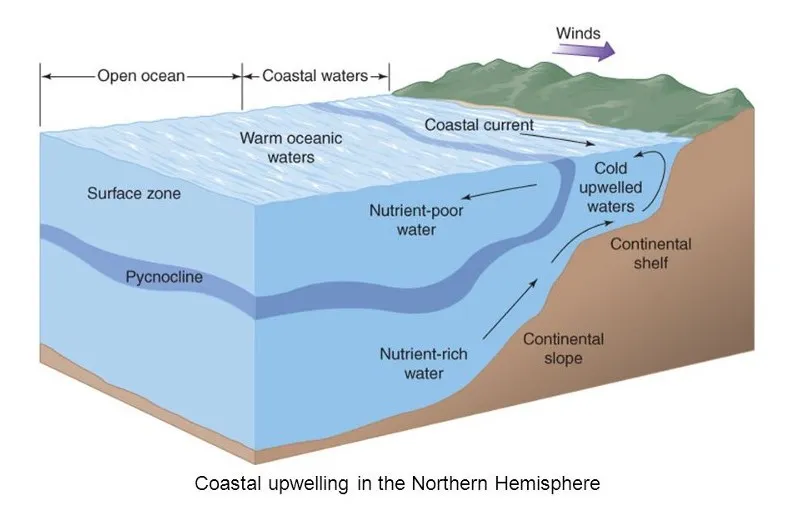
\includegraphics[width=1.0\textwidth]{figures/Chap1CoastalUpwelling.png}
	\caption{Conceptual model of wind-driven upwelling process in the northern hemisphere. It should be noted that in the southern hemisphere, the wind direction is reversed but generates the same upwelling effect.}
	\label{Chap1CoastalUpwelling}
\end{figure}

The process of upwelling can be measured using an index ($upwelling index = \mu \left ( cos\theta -\tau  \right )$) presented by \cite{FielDavi1989}, where $\mu$ represents the wind speed ($ms^{-1}$), $\theta$ represents the wind direction in degrees, and $\tau$ is the orientation of the coastline. This process has important ecological consequences only if parcels of water transported from the bottom to the photic zone are rich in nutrients. This occurs in what are called upwelling systems, of which the area off Peru is one of the most important \citep{ChavBert2008}, although  a global trend of decreasing primary productivity has been shown in the last decades \citep{Dema2009,RoxyModi2016} and in climate change scenarios \citep{BlancJenn2012,KulkPlat2020}, which could potentially jeopardize the amount of primary production required to sustain global fisheries \citep{PaulChri1995}, especially the Peruvian anchovy fishery, which has had an historic collapse in the past \citep{AriaNiqu2011,Aria2012}, and could play an important role in the food security of the Peruvian people \citep{MajlDela2017}. We also know that the environmental conditions in which the Peruvian anchovy develops are favorable, although they also present great variability in the northern zone of the Humboldt current.\\

Understanding upwelling systems is essential for managing fisheries, studying climate impacts in the past and the future \citep{BakuBlac2015,DiLo2015,TimZori2016}, and preserving the health of marine ecosystems, understood as ``the condition of a system that is self-maintaining, vigorous, resilient to externally imposed pressures, and able to sustain services to humans \citep{TettGowe2013}''.\\

\begin{figure}[H]
	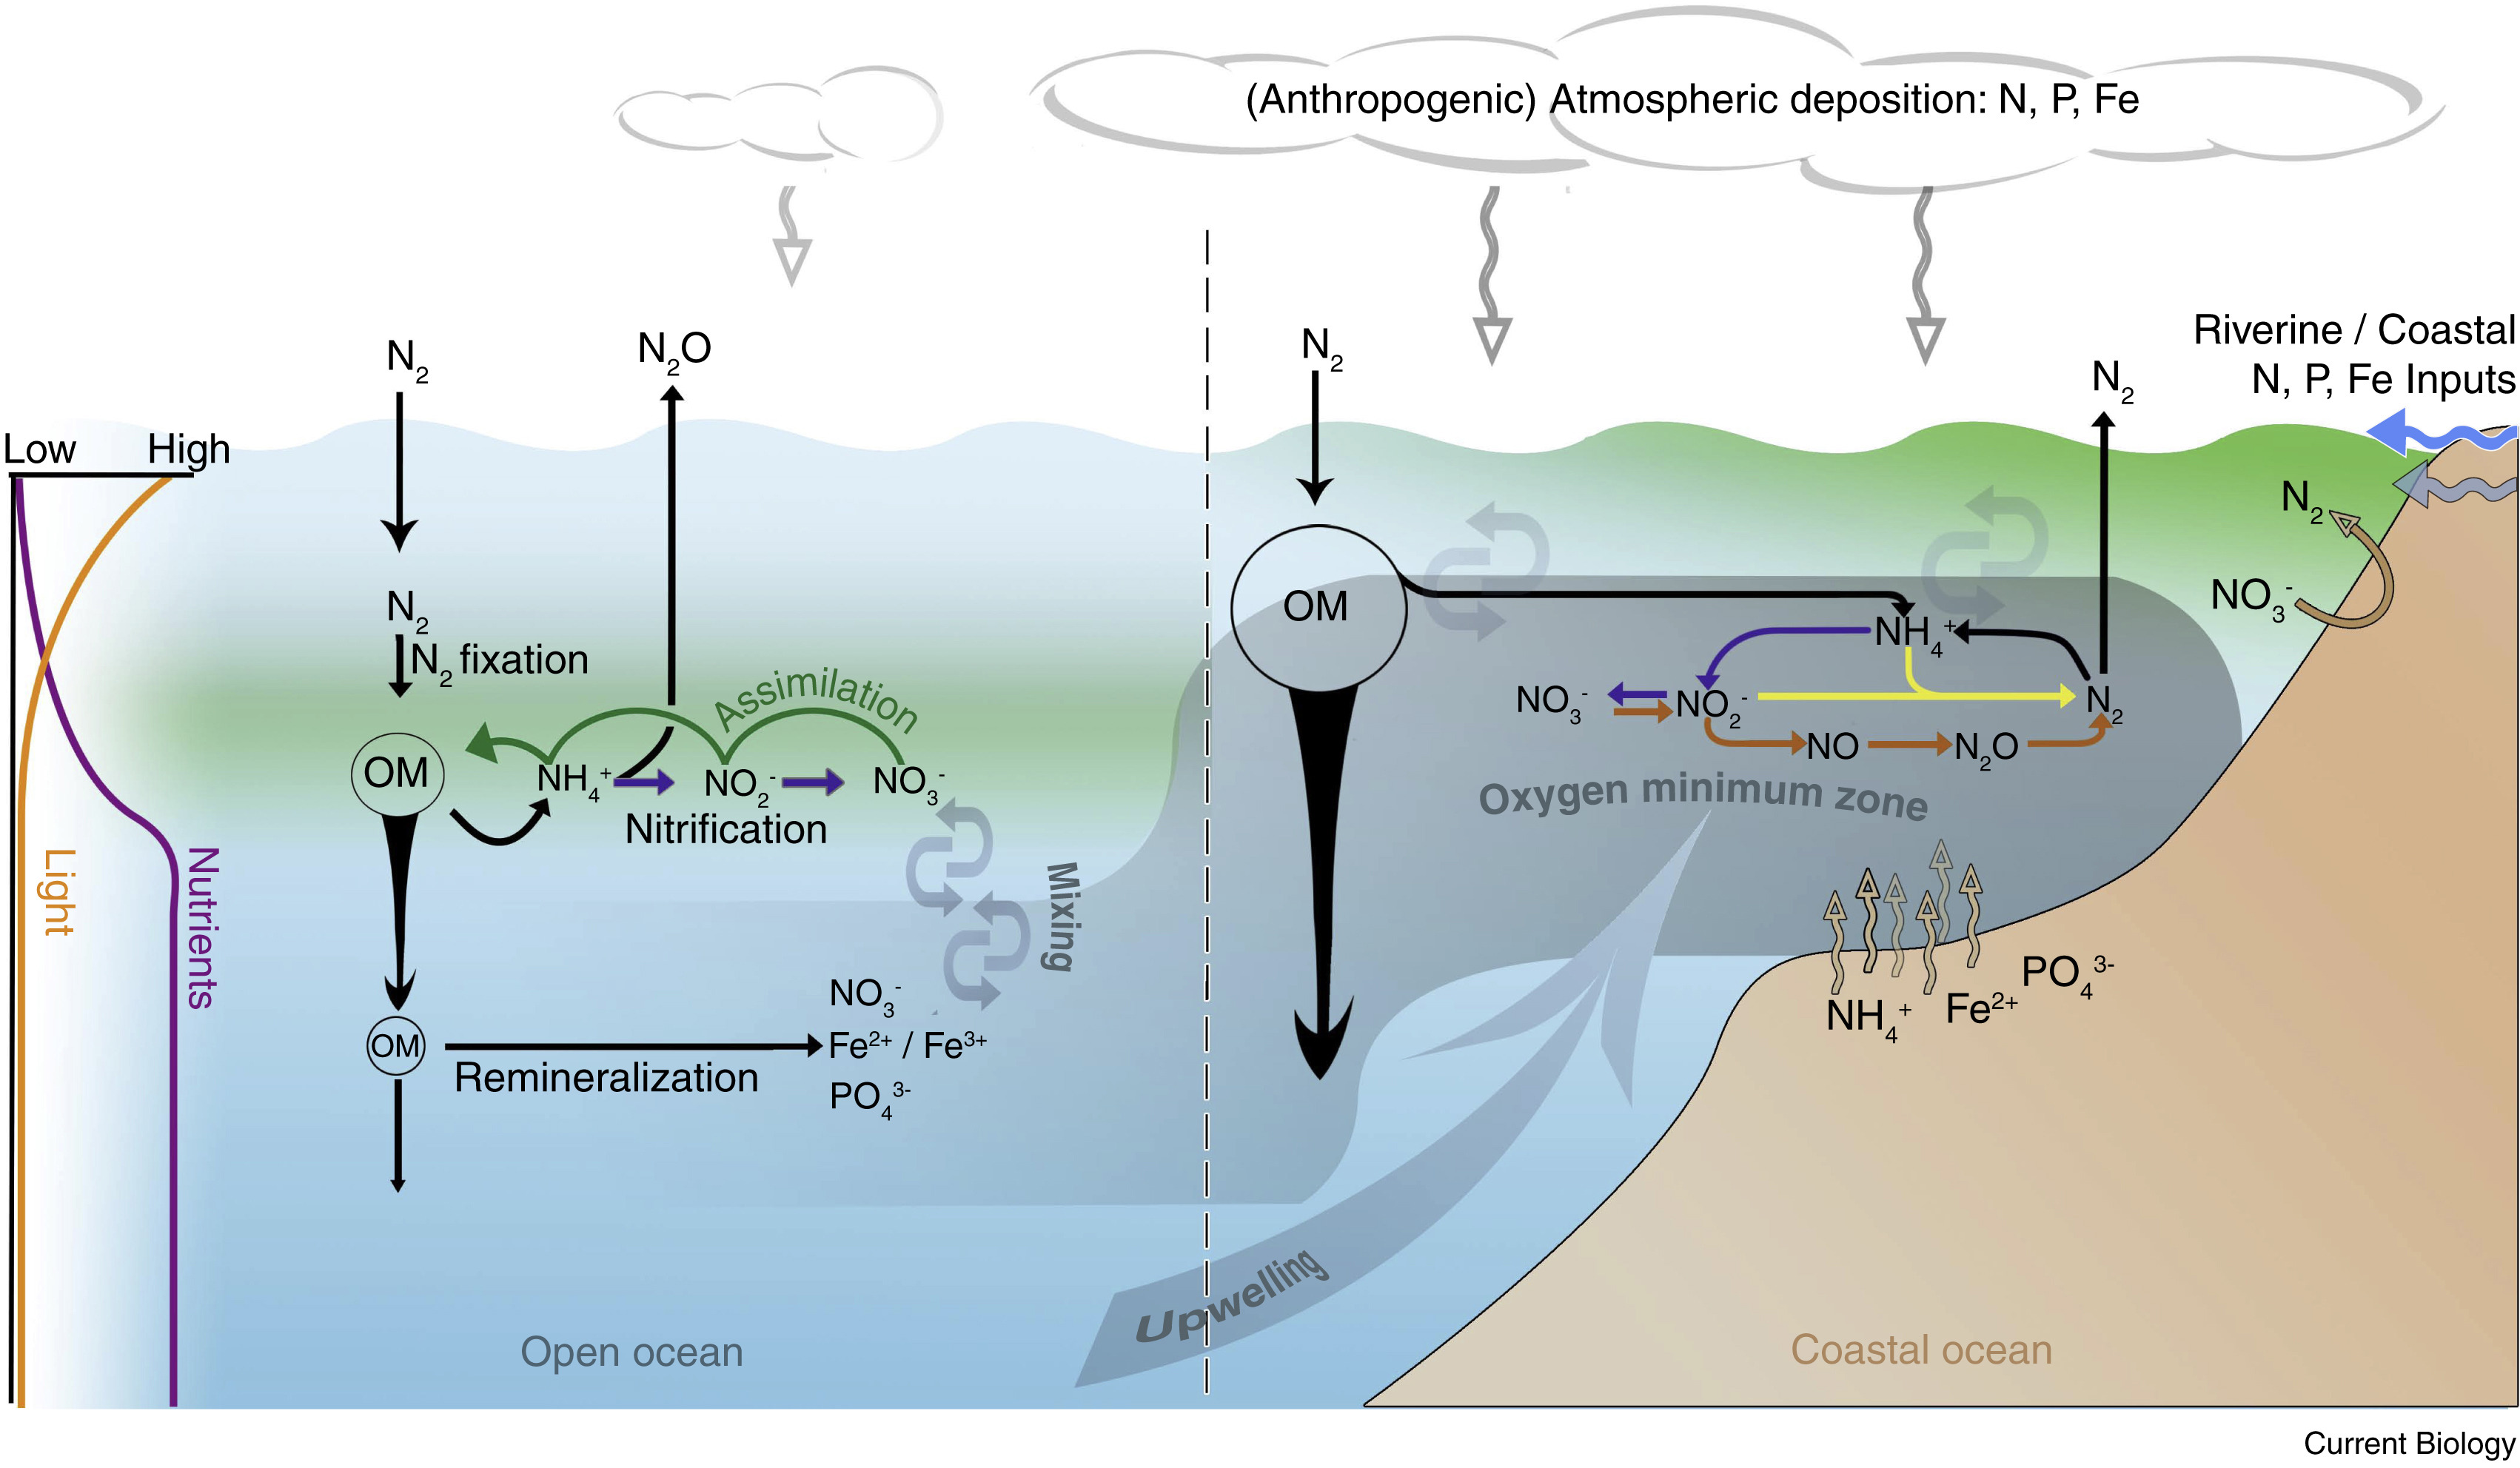
\includegraphics[width=1.0\textwidth]{figures/Chap1UpwellingFertilization.jpg}
	\centering
	\caption{Scheme of fertilization sources to the ocean as well as upwelling, riverine discharges and atmospheric deposition. The figure was taken from \cite{BrisMohr2017}.}
	\centering
	\label{Chap1UpwellingFertilization}
\end{figure}

\clearpage
\section{The northern Humboldt Current system (NHCS)}\label{Chap1NHCS}

The connection between ancient Peruvian coastal inhabitants and the sea has been apparent since pre-Columbian times \citep{Prie2014,Prie2019}. Ancient civilizations utilized the marine resources of the Peruvian coast, including a variety of fish species such as engraulids, which were dried and salted for easier transportation \citep{MarcSomm1999}. They also harvested bivalve mollusks and gastropods \citep{ChicRoja2013,WeinOsbo2022}, and macroalgae \citep{AvilPadi2020}. All of these resources flourished under the influence of the \acrfull{nhcs} and continue to generate a significant positive economic impact. Then, it is important to understand the characteristics that make this marine ecosystem unique.\\

The \acrshort{nhcs} is one of the most productive systems in the world (Fig. \ref{Chap1UpwellingSystems}), mostly located off the Peruvian coast (70\textdegree $W$ – 90\textdegree $W$; 0\textdegree $S$ – 20\textdegree $S$) and is part of the broader Peru-Chile upwelling system \citep{GradChai2018,TaraArnt2001}. \acrshort{nhcs} is considered as a highly productive marine ecosystem with a productivity of $>$ 300 $gC/cm^{2}/yr$ \citep{KampCap5}, largely due to the regular presence of upwelling-favorable winds throughout the year from 5\textdegree $S$ to 26\textdegree $S$, a feature that is rather seasonal beyond 26\textdegree $S$ \citep{BelmEche2014}. There is however seasonal and interannual variability in upwelling intensity, with intensification in the later part of the $20^{th}$ century (1960 – 2001) \citep{NaraPaul2010}.\\

\begin{figure}[ht]
	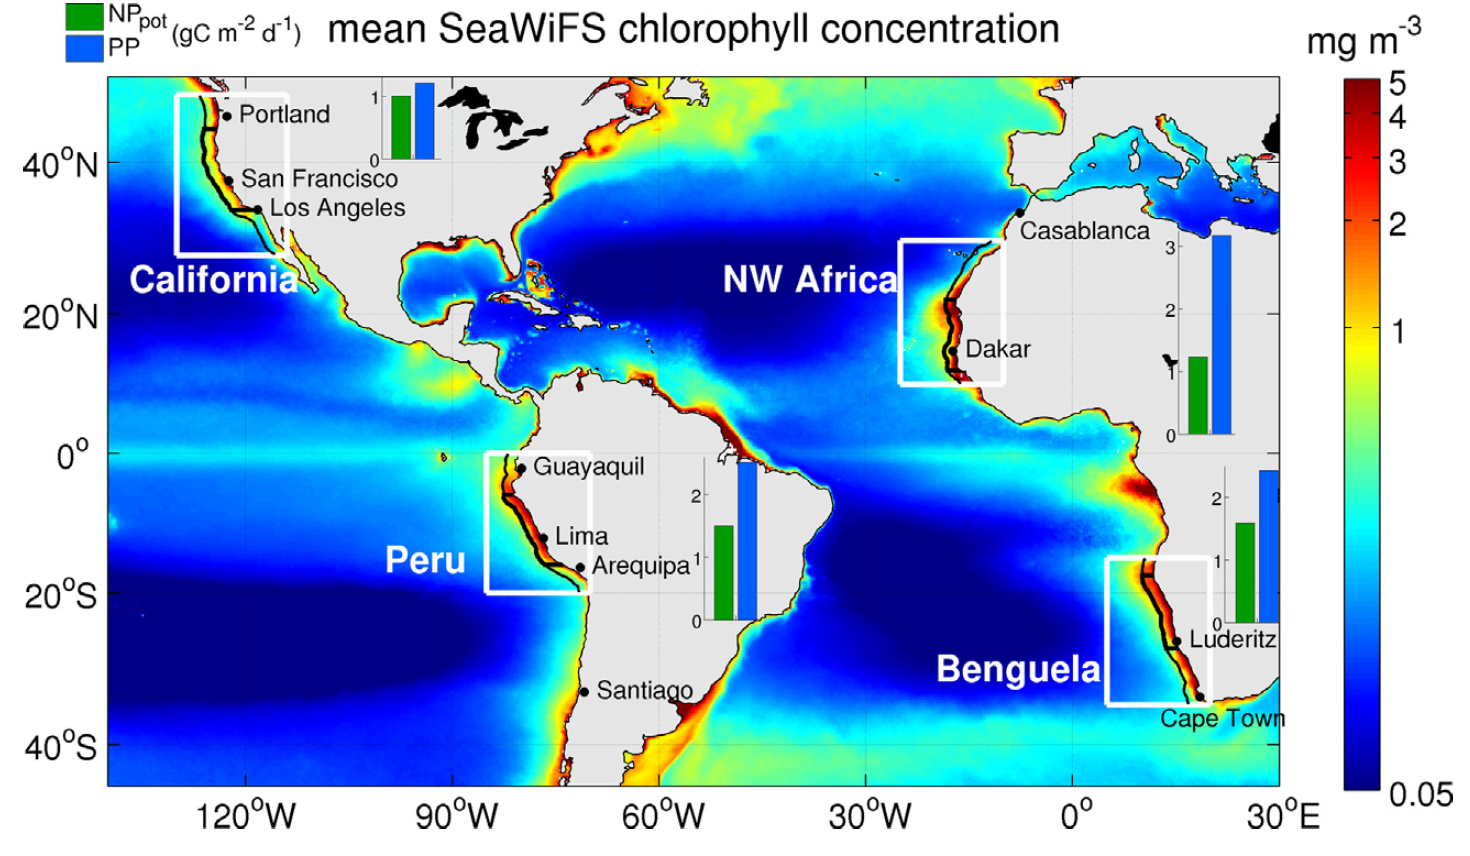
\includegraphics[width=1.0\textwidth]{figures/Chap1UpwellingSystems.png}
	\centering
	\caption{Scheme of the four most important upwelling systems represented by chlorophyll concentration measured by satellite images. The figure was taken from \cite{MessChav2015}.}
	\label{Chap1UpwellingSystems}
\end{figure}

In the \acrshort{nhcs}, water masses from different origins with specific temperature and salinity ranges converge \citep{SilvRoja2009,MontCola2010,ChaiDomi2013}. The following water masses are currently distinguished off Peru: \acrfull{tsw}; \acrfull{esw}; \acrfull{stsw}; \acrfull{essw}; \acrfull{espiw}; \acrfull{aaiw} \citep{GradChai2018}. Details of temperature and salinity range of these water masses are reported in Table \ref{TabWaterMasses} and Fig. \ref{Chap1WaterMassesNHCS}. These water masses are transported by several surface [\acrfull{epcc}; \acrfull{pcc}; \acrfull{sec}; \acrfull{poc}] and subsurface currents [\acrfull{euc}; \acrfull{pcuc}].\\

The mean circulation shows both poleward and equatorward flows (Fig. \ref{Chap1MeanCirculationNHCS}). The upper layer ($\sim$ 25 $m$) close to the coast shows a relatively strong poleward flow ($\sim$ 20 - 30 $cm/s^{-1}$) associated with the \acrshort{epcc} transporting relatively warm and fresh \acrshort{esw}. At $5$\textdegree $S$, the \acrshort{epcc} separates into two branches, one feeding the westward \acrshort{sec} and the other one continuing southward weakening until $\sim$ 8\textdegree $S$ – 9\textdegree $S$.\\

\begin{table}[ht]
\centering
\begin{tabular}{c|c|c}
\hline
\textbf{Water mass}								&
\textbf{Temperature range (\textdegree $C$)}	&
\textbf{Salinity range ($S$)}					\\
\hline
TSW				& 
23.5 - 24.5		& 
33.5 – 34.4		\\
ESW				& 
20.0 – 24.0		& 
34.6 – 35.0		\\
STSW				& 
19.0 – 23.5			& 
\textgreater{35.4}	\\
ESSW			&
8.0 – 14.0		&
34.6 – 35.0		\\
ESPIW			& 
12.0 – 14.0		& 
34.8			\\
AAIW			& 
4.0 – 7.0		& 
34.5 – 34.6		\\
\hline            
\end{tabular}
\caption{Temperature ($T$, in \textdegree $C$) and salinity ($S$) ranges of the main water-masses in the \acrshort{nhcs}. \acrfull{tsw}; \acrfull{esw}; \acrfull{stsw}; \acrfull{essw}; \acrfull{espiw}; \acrfull{aaiw}. Table modified from \cite{GradChai2018}.}
\label{TabWaterMasses}
\end{table}

Further south there is equatorward flow associated with the \acrshort{pcc} and the \acrshort{poc} transporting cold waters. The middle layer (100 – 200 $m$) is predominantly a poleward flow influenced by the \acrshort{pcuc} that extends along the entire coast, transporting \acrshort{essw} with a mean velocity that can locally reach 20 $cm/s^{-1}$. In the deeper layer (500 $m$), the average circulation is mainly equatorward transporting relatively fresh and cold \acrshort{aaiw}  \citep{ChaiDomi2013,PietTest2013}.\\

\begin{figure}[ht]
	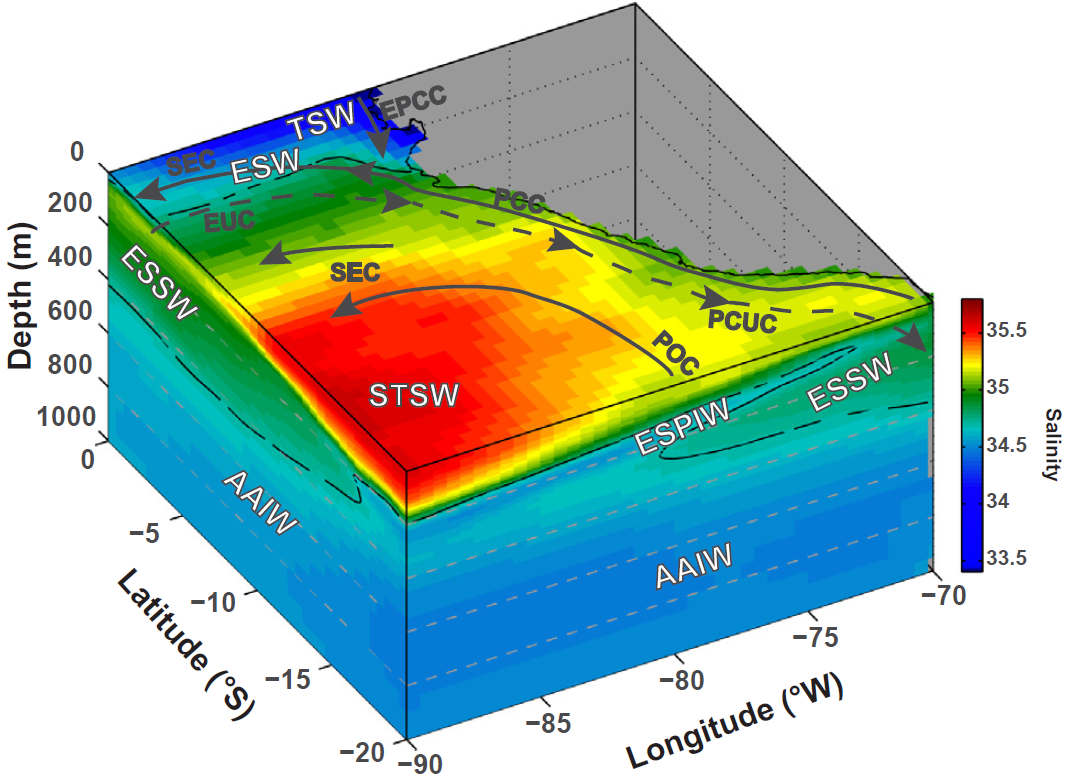
\includegraphics[width=1.0\textwidth]{figures/Chap1WaterMassesNHCS.png}
	\centering
	\caption{Main water-masses of the \acrshort{nhcs}. The color corresponds to the salinity range. The surface (thick solid lines) and subsurface (thick dashed lines) currents: \acrfull{epcc}; \acrfull{pcc}; \acrfull{sec}; \acrfull{poc}; \acrfull{euc}; \acrfull{pcuc}. Figure taken from \cite{GradChai2018}.}
	\label{Chap1WaterMassesNHCS}
\end{figure}

The mean temperature in the coastal zone off Peru is 17.6\textdegree $C$ \citep{MontPurc2003} but temperature shows strong seasonal and interannual variability, particularly due to El Ni\~{n}o events that can generate positive anomalies of more than 6\textdegree $C$  \citep{BraiMcla1987,SancCali2000,CaiBorl2014,CaiWang2017,CaiWang2018,FreuHenl2019}, and other extreme events referred to as ``coastal Ni\~{n}o" \citep{EcheCola2018,Garr2018,HuHuan2019,RodrDiaz2019,TakaMart2019}, although the above warm events could be more generally categorized as marine heatwaves, this term better describes their characteristics and physical mechanisms \citep{PietCola2021}. Along the Peruvian coast, the seasonal variability of temperature increases from north to south. This is associated with a smaller effect of upwelling in the northern zone than in the south \citep{BraiMcla1987}.\\

\begin{figure}[ht]
	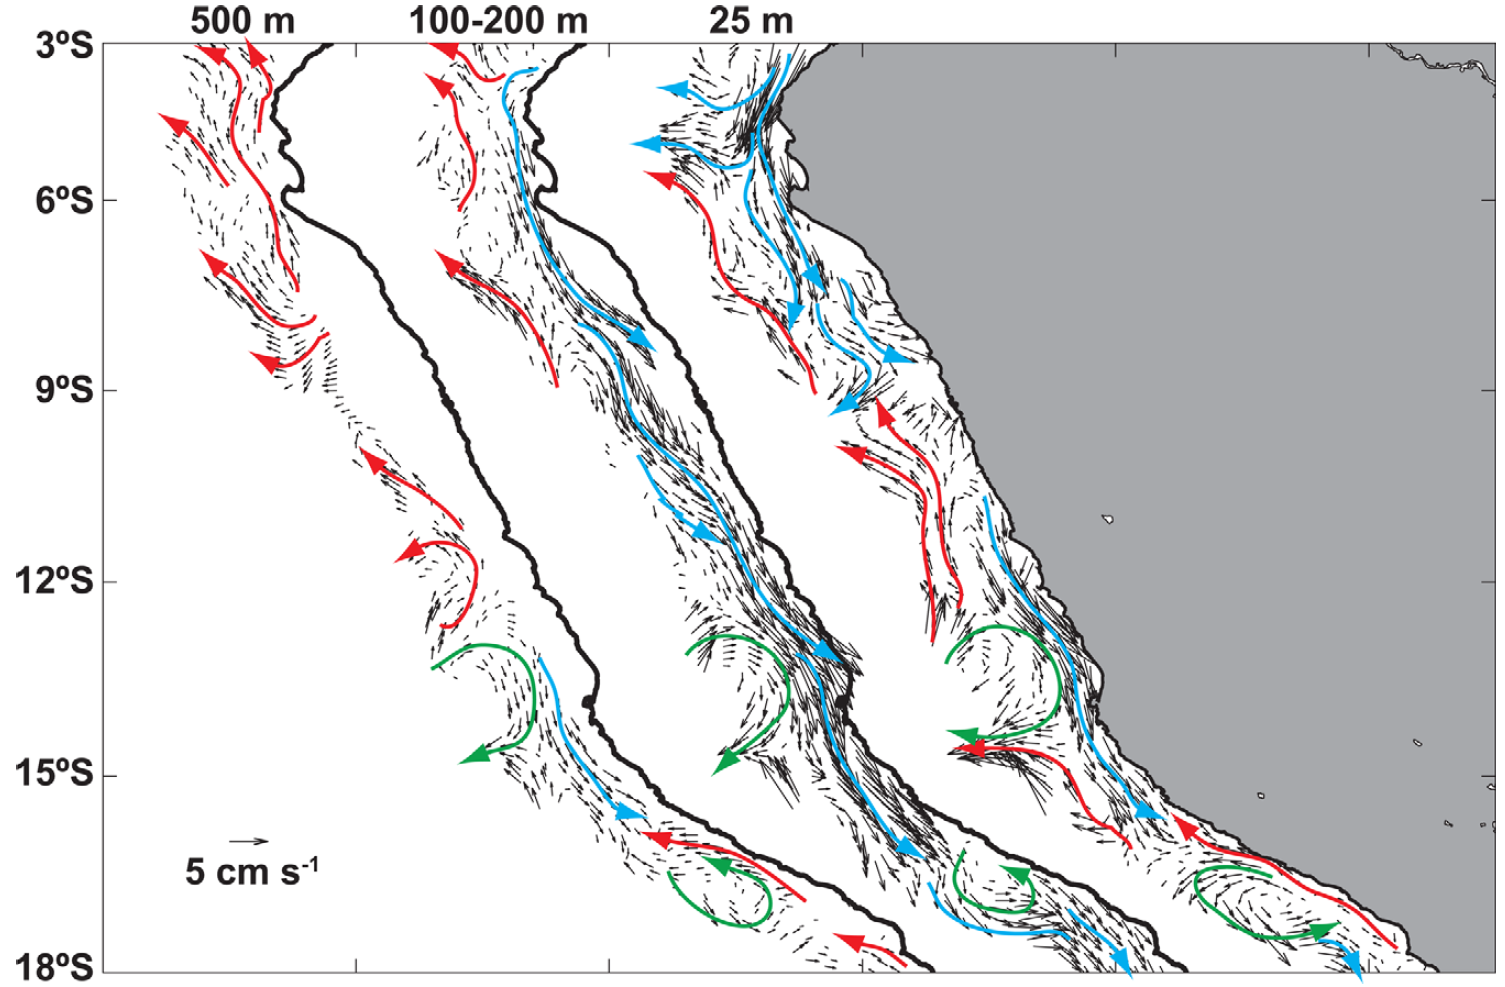
\includegraphics[width=0.8\textwidth]{figures/Chap1MeanCirculationNHCS.png}
	\centering
	\caption{Mean circulation at 25 $m$, between 100 $m$ and 200 $m$, and 500 $m$ depth. Red and blue arrows represent the equatorward and poleward flows, respectively. Green arrows indicate the presence of mesoscale cyclonic ($\sim$ 14\textdegree $S$) and anticyclonic ($\sim$ 17\textdegree $S$) eddy-like features. Figure taken from \cite{ChaiDomi2013}.}
	\label{Chap1MeanCirculationNHCS}
\end{figure}

Dissolved oxygen also shows a high spatiotemporal variability, which may at time limit the generally well oxygenated layers located near the surface \citep{EspiEche2017,EspiEche2019}. Then, \acrlong{omz} is defined as a region of the ocean exhibiting a pronounced deficiency in oxygen concentration within the water column. These zones are characterised by the presence of three distinct layers: the oxycline (upper oxygen gradient), the core (typically exhibiting oxygen concentrations below 20 $\mu M$) and the lower oxygen gradient, with eddy fluxes which contribute to the ventilation of the Peruvian oxygen minimum zone \citep{BettLope2015}. Consequently, the oxygen dynamics off the Peruvian coast can result in scenarios with a markedly low oxygen presence, which in turn reduces and limits the environment available for plankton aggregation to a depth range of 0 to 65 $m$ in the slope zone and may even be reduced to a depth range of 20 to 35 $m$ in the shelf break zone. This can result in an unusually high presence of zooplankton at the surface, which may then dissipate once the low oxygen event is overcome \citep{Judk1980}. It would appear that there is a relationship between the depth of the oxycline, macrozooplankton and forage fish (\textit{\gls{ringens}}) that can be observed at different scales, from tens of kilometers to a few hundred meters providing evidence that the submesoscale-to-mesoscale variability of the oxycline depth drives the distribution of macrozooplankton, then, shaping distribution structures of forage fish \citep{GradFabl2012,GradBert2016}.\\

Phytoplankton is consumed primarily by zooplankton, which in turn is preyed upon by small pelagic fish. These groups of organisms are subject to significant fluctuations due to seasonal and interannual (El Ni\~{n}o) physical fluctuations in oceanographic conditions. Chlorophyll, used as a proxy for primary productivity (phytoplankton), shows an annual signal, which is favored by wind stress, exhibits a seasonal maximum that shifts southward from spring to summer. This signal is in phase with the seasonal maximum in $Chl-a$ concentration detected by satellite off the coast of Chile. However, off Peru, this signal is not in phase, exhibiting seasonal maxima of $Chl-a$ in summer and the intensity of upwelling in winter \citep{EcheAumo2008,CorrHorm2012}. The spatial distributions of certain zooplankton groups exhibit a high degree of correlation with surface water masses, circulation patterns, and upwelling regions. This correlation is consistent with the ecological and dynamic partitioning of the pelagic ecosystem \citep{FernFarb2006}. However, in comparison to Peru, the signal corresponding to zooplankton is more complex, exhibiting temporal and spatial variations at different scales, with spring and summer being the most significant \citep{AronAyon2009,AronGrad2019}.\\

Thus, water masses intermingle along the coastline following the currents and constitute the biotope of one of the most productive ecosystems in the world. The \acrfull{spf} reproduce by dispersing their eggs in the surface layers, and are therefore particularly exposed to the fluctuations of this biotope which will determine in large part their chances of survival. In the following section we will describe the main species of \acrshort{spf} that inhabit this ecosystem, the Peruvian anchovy.\\

\clearpage
\section{The Peruvian anchovy (\textit{Engraulis ringens}, Jenyns 1842)}\label{Chap1PeruAnch}

Clupeoid fishes are present in pelagic environments worldwide, particularly in the productive coastal upwelling regions along the eastern margins of the Atlantic and Pacific oceans. The largest stocks are usually composed of species such as sardine, pilchard, and anchovy (\textit{Sardinops spp.} and \textit{Engraulis spp.}). The schooling behavior of clupeoids makes them easy to catch with purse seiners, resulting in some populations reaching enormous biomasses and becoming important economic resources. For example, during the early 1970s, clupeoids, particularly the Peruvian anchoveta (\textit{\gls{ringens}}), contributed approximately one-third of the world's total catches, which were around 65 million tonnes at the time \citep{ColeMcGl1998}.\\

Fig. \ref{Chap1Engraulis_ringens} shows a schematic representation of \textit{\gls{ringens}}, a \acrshort{spf}, catalogued as \textit{r}-selection species \citep{Pianka1970}, with a slightly compressed elongated body, long head, prolonged snout and very large eyes. In the dorsal part its color is dark blue, while in the ventral part it is silver \citep{Whit1988}.\\

Taxonomically, according to \acrlong{itis} (\href{https://www.itis.gov/}{ITIS}), \textit{\gls{ringens}} is located in the evolutionary tree as follows:\\

\begin{itemize}
  \centering
  \item Kingdom: Animalia
  \item Phylum: Chordata
  \item Subphylum: Vertebrata
  \item Infraphylum: Gnathostomata
  \item Superclass: Actinopterygii
  \item Class: Teleostei
  \item Order: Clupeiformes
  \item Family: Engraulidae
  \item Genus: Engraulis
  \item Species: \textit{\gls{ringens}}, Jenyns, 1842
  \item Common name: Peruvian anchovy
\end{itemize}

\begin{figure}[!]
	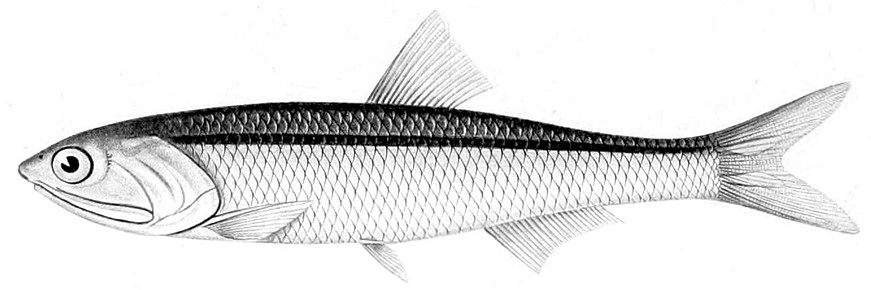
\includegraphics[width=1.0\textwidth]{figures/Chap1Engraulis_ringens.jpg}
	\centering
	\caption{Schematic representation of an adult Peruvian anchovy (\textit{\gls{ringens}}).}
	\label{Chap1Engraulis_ringens}
\end{figure}

\textit{\gls{ringens}} can reach a maximum size of 20 $cm$ and has a life span of 4 years. Its first sexual maturity may be at a size of 12 $cm$ \citep{GutiSwar2007,MarzShin2009}. This species performs external fertilization by formation of spawning aggregations, which warrants synchrony in the timing of gamete production and optimizes fertilization rates. Females release the eggs into the environment so that males can fertilize them without the need for copulation \citep{Gani2014}. During the main period of annual spawning in August-September, 16.04 \% of the female population of the central and northern anchovy stock off Peru spawned per day, this means that on average, every female spawned a new batch of eggs every 6.23 $days$ \citep{AlheAlar1984,AlheAleg1983}. In unfavorable environmental conditions, a female is capable of reabsorbing part of the ovigerous mass to obtain energy, a phenomenon known as atresia \citep{PereRoqu2008,EspiVera2009,ClarCast2012,BuitPere2018}. This species has two important spawning peaks off Peru, summer and winter, but a significant presence of eggs and larvae is reported throughout the year \citep{MarzShin2009}. Anchovy in Peru has a mainly zooplanktivorous diet, with ontogenetic and spatiotemporal variability in prey preferences, with an increase in the contribution of euphausiids to the diet as \textit{\gls{ringens}} increases in size up to 85 \% of their diet as adults (18 – 20 $cm$), in contrast, their consumption of calanoid copepods decreases with size, while diatoms make up a minimal part of their diet throughout their life span \citep{EspiBert2008,EspiBert2014}.\\

In the natural environment, eggs of \textit{\gls{ringens}} are pelagic and transparent. Their shape is ovoid, with an average major axis of 1.42 $mm$ and a minor axis of 0.71 $mm$. However, there is latitudinal variability associated with the size of the eggs, which are protected by a smooth membrane. Following hatching, the larva exhibits no pigmentation, but rather an elongated yolk sac that terminates at the posterior end of the intestine. Its body is cylindrical, with a head that is somewhat wider than the body and lacks differentiation of the mouth or jaw \citep{EinaRoja1963}. \textit{\gls{ringens}}’s early life description \citep{RiouOfel2021}, currently distinguishes 4 stages: \textbf{stage $\mathbf{1}$} from hatching to 2 \acrfull{dph} there are transparent yolk-sac larvae with closed mouth and eyes and non-pigmented body. Stage 1 ends with the opening of the mouth, pigmentation of the eyes and remnants of the yolk-sac (at length ranging from $\sim$ 2 - 4 $mm$ depending on temperature); \textbf{stage $\mathbf{2}$} from the complete absorption of the yolk sac at 3 \acrshort{dph} until larvae are between 12 - 19 \acrshort{dph} with length ranging from 8.15 - 12.97 $mm$; \textbf{stage $\mathbf{3}$} included larvae between 19-26 \acrshort{dph} and corresponding length from 10.89 - 15.03 $mm$; \textbf{stage $\mathbf{4}$}, from 33 \acrshort{dph}, larvae showed melanophores developed on the head and body, with visible gills. The first sign of schooling (continuous swimming as a group and clear evidence of active swimming behaviour, \cite{Shaw1962}) also occurred at this stage (31 \acrshort{dph}).\\

After the larval stage, anchovy juveniles already have the definitive adult form and from 12 $cm$ of length, they became available for industrial fishery \citep{MarzShin2009}. This industrial fishery is oriented almost entirely (98 \%) to indirect human consumption (feed fish) and only 2 \% is intended for direct human consumption (food fish) in canned, cured, frozen or fresh presentations \citep{FreoSuei2014}.\\

\textit{\gls{ringens}} fishery management is based on scientific monitoring of adult population indicators determined by acoustic surveys \citep{GutiSwar2007} or by the daily egg production method \citep{Ayon2000}, then allocating fishing quotas to each registered vessel and catching monitoring by technical research personnel on board these vessels \citep{KroeSanc2019}. Thus, the Peruvian anchovy has become one of the most abundant and at the same time the most studied fishery, but understanding the impact of environmental conditions on the early-life stages of anchovy and further population dynamics remains challenging.\\

\begin{figure}[!]
	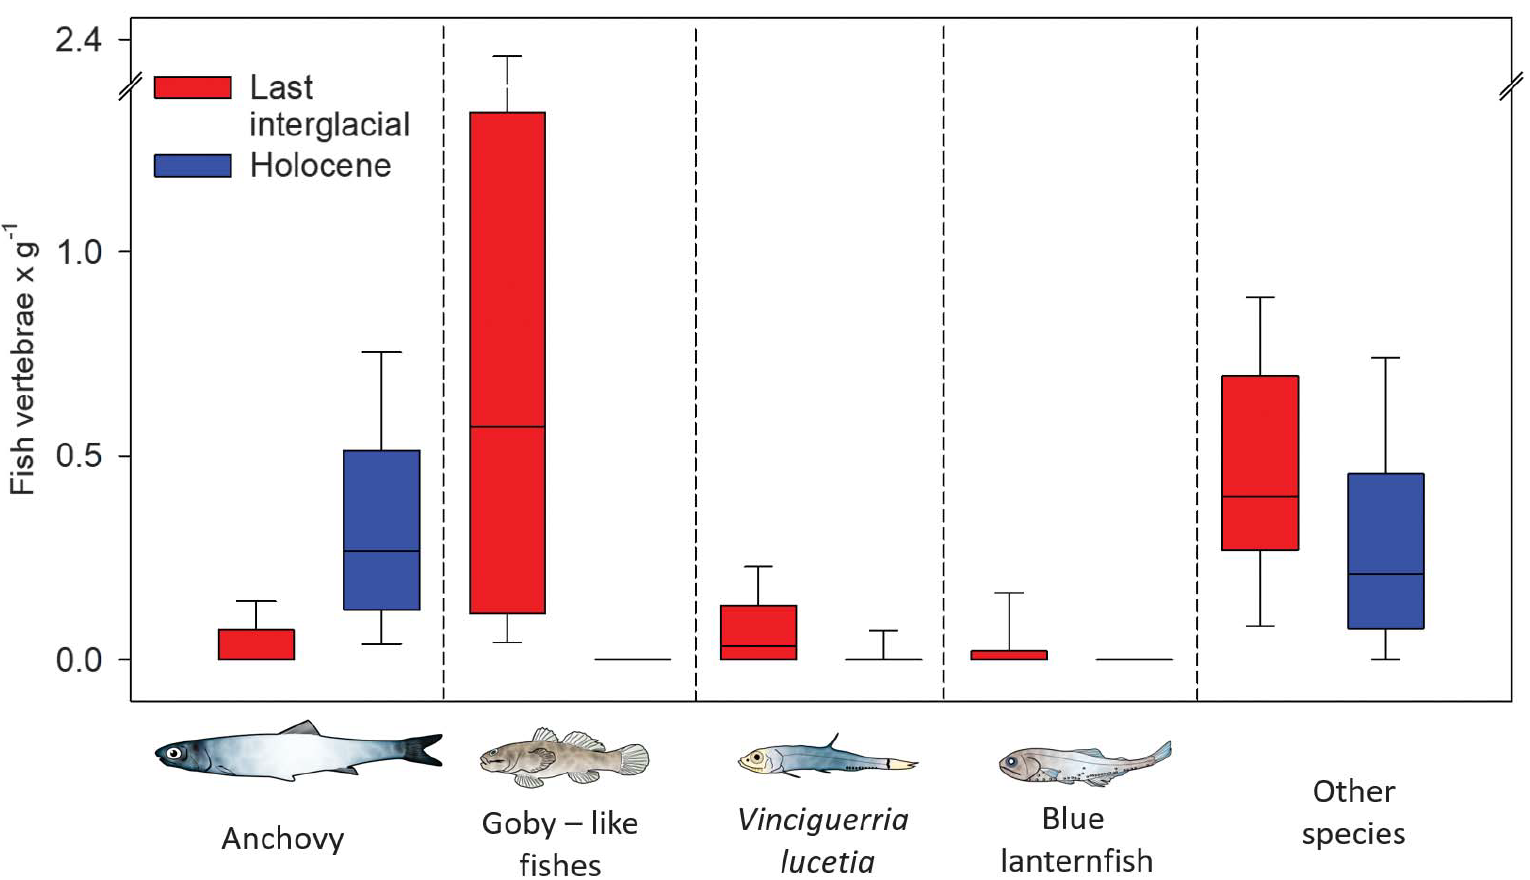
\includegraphics[width=1.0\textwidth]{figures/Chap1VertebraeAbundances.png}
	\centering
	\caption{Fish vertebrae abundances during the last interglacial and Holocene. Figure taken from \cite{SalvSchn2022}.}
	\label{Chap1VertebraeAbundances}
\end{figure}

However, this abundance has not been constant at geological scales as shown by palaeoceanographic records, which have evidenced that \textit{\gls{ringens}} has populated the \acrshort{nhcs} for thousands of years under a naturally varying climate with high variability during the last 25 $ky$ \citep{SalvField2018,SalvGuti2019,SalvSchn2022}, playing an important role transferring energy from lower to higher levels of the food web \citep{ChecAsch2017}. Fig. \ref{Chap1VertebraeAbundances} show we are currently in the Holocene period, characterized by a great abundance of the Peruvian anchovy biomass, however, during the last interglacial period, with warm and oxygen-poor environmental conditions, the presence of \textit{\gls{ringens}} was considerably lower, and that conditions favored the flourishing of other mesopelagic fishes \citep{SalvSchn2022}, environmental conditions that could be repeated in a climate change scenario \citep{EcheGeva2020}.\\

Thus, environmental variability in a complex system such as the \acrshort{nhcs} and its impact on \textit{\gls{ringens}} abundance has been extensively studied under different approaches, one of them being modelling.\\

\clearpage
\section{Modelling studies on \textit{E. ringens}}\label{Chap1ModeAnch}

The inherent impossibility of monitoring the entire ecosystem at high frequency and resolution is a major limitation of ichthyoplankton in situ observations. This is where models, become relevant, allowing us to integrate multiple spatio-temporal scales and to testing hypotheses on ichthyoplankton dynamics in response to the different  environmental forcing’s, including forecasting scenarios \citep{GearDode2020}.\\

Despite many modelling studies conducted in the past \citep{LettPenv2007,BrocLett2008,GutiRami2008,OlivPena2011,XuChai2013} that have tried to explain a relationship between environmental variability and the success of anchovy recruitment, much remains to be understood due to the high plasticity of this species and its adaptation capacity to environmental changes \citep{EspiBert2008,EspiBert2014,CanaAdas2018,PlazCern2018}.\\

Early modelling studies for the understanding of \acrshort{nhcs} dynamics were done by hydrodynamic modelling reproducing general ocean circulation patterns \citep{PenvEche2005,ColaMcwi2012}, its interannual variability \citep{ColaCape2008,EspiEche2017}, its potential changes under future climate scenarios \citep{OerdCola2015,EcheGeva2020}. These previous works provide us a strong physical basis for ecological studies in the \acrshort{nhcs}.\\

From a realistic representation of the physical environment, researchers have tested \cite{Baku1998} triad hypothesis for \acrshort{spf} recruitment and early life stages survival by quantification of enrichment, concentration and retention processes in \acrshort{nhcs} \citep{LettPenv2007} and complementarily also in the Benguela upwelling ecosystem \citep{LettRoy2006}, in both cases, the coastal zone emerged as the most favorable by analyzing the spatial distribution and seasonal variability of these indices. Further modelling studies showed that \textit{\gls{ringens}} larval retention patterns displayed strong seasonal variability possibly modulated by vertical distribution of individuals in regards to the vertical current structure, resulting in a maximal coastal retention close to the surface in winter and in deeper layers in summer. Also, a partial match between dates and locations of enhanced retention and observed egg concentration patterns was found \citep{BrocLett2008}. Additionally, in the region of Chile where the same species also thrives, a study was conducted to examine the transport of eggs and larvae from spawning zones in central Chile to historical nursery areas. The results indicated that the highest pre-recruitment values were mainly found in winter \citep{ParaCola2012}.\\

In the four main \acrfull{ebus}, the reproductive strategy of \acrshort{spf} species, dominated by anchovies and sardines, is a trade-off between larval retention and larval food availability. In the \acrshort{nhcs}, the winter spawning benefit both from high zooplankton and shelf retention rates, which may explain the particularly  large \acrshort{spf} populations \citep{BrocCola2009,BrocLett2011}. Climate change might negatively impact \textit{\gls{ringens}} recruitment due to a reduction in the size of the habitat due to a reduction in ecosystem productivity not compensated by increased retention rates \citep{BrocEche2013}. The effects of temperature and food availability on larval growth could modulate this result; as it was suggested that \acrfull{enso} events may negatively impact \textit{\gls{ringens}}  recruitment by reducing the larval growth speed due to changes in food availability \citep{XuChai2013,XuRose2015}. The seasonal variability in larval growth speed was not explicitly taken into account in previous studies, a gap that was addressed in the present work.\\

In order to investigate the impact of environmental variability on early life stages of \acrshort{spf}, we developed \gls{ich-deb}, an individual-based model \citep{LettVerl2008} including larval retention processes and a \acrfull{deb} \citep{Kooi2009} bioenergetic module for larval growth. Using this tool, we assessed the effect of hydrodynamic simulations horizontal resolution on simulated larval retention patterns in chapter \ref{Chap2}, then, we studied the impact of the biological processes on simulated larval growth and recruitment and the effect of the upper thermal limit in chapter \ref{Chap3}, for which lab experiments are lacking. Finally in chapter \ref{Chap4} and \ref{Chap5}, we presented a complete life cycle growth model of the Peruvian anchovy with potential uses for the study of juvenile and adult behaviour.\\

\clearpage

%\section{The recruitment problem}\label{Chap1RecruProb}
%Fish populations can vary greatly over time, from interannual to millennial fluctuations. For short-lived fish, these two scales of variability are comparable in magnitude, indicating that reproductive success and recruitment are the main factors contributing to abundance. Reproductive success refers to the number of offspring an individual produces per breeding event or over their lifetime, which is closely related to the environment in which the parents develop and is something that can be monitored through research cruises during the spawning season, and in the other hand to address the ``recruitment problem'', which is the lack of knowledge to explain recruitment variability, a solid theoretical basis and practical methods are necessary, however, monitoring early life stages in the natural environment is inherently difficult, posing a great challenge with more questions than answers.
%
%Theories on how environmental conditions affect recruitment success, based on the survival/mortality of early life-history stages, can be categorized into mechanistic and synthesis theories. Mechanistic theories focus on particular physical processes, while synthesis theories aim to integrate the various mechanistic processes into a single conceptual framework. Although some theories have been successfully tested, there has been little success in reliably predicting recruitment success based on environmental conditions \citep{ColeMcGl1998}.
%\clearpage


\mainmatter
\linenumbers

\chapter{Effect of horizontal resolution on simulated larval retention patterns}\label{Chap2}

\section{Introduction}\label{Chap2Intro}

Interest in the early life stages of marine organisms has increased \citep{Stra1993,Haven1995,Levi2006,GawaMoni2007,CoweSpon2009} in particular for understanding larval transport and dispersal patterns \citep{Youn1995,GreeMayp2015,Leis2021} due to their key role in the ecology of marine organisms \citep{MoseSmit1993} and potential usefulness in decision making for the management of marine protected areas (MPA) \citep{DaloBogd2015}. Many marine species have pelagic early life stages in their life cycle \citep{Haven1995}. This phase of locomotion is essentially driven by ocean currents and species-specific vertical behaviours \citep{Levi1990,CowePari2006,DaloBogd2015}.\\

In the case of sessile organisms, such as scallops and corals, concepts such as larval transport, larval dispersal and population connectivity have been formally defined \citep{PineHare2007}. Hence, \textbf{larval transport} is the horizontal translocation of a larva between points $X_{1}Y_{1}$, and $X_{2}Y_{2}$, where $X$ and $Y$ are the horizontal axes, perpendicular and parallel to the coastline respectively (to simplify, this definition ignores the vertical axis $Z$). On the other hand, \textbf{larval dispersal} refers to the spread of larvae from a spawning source to a settlement site (a geographic point from which the adult will have limited or no mobility). We note that larval transport is a component of larval dispersal (Fig. \ref{Chap2LarvalTransport}). Finally, \textbf{population connectivity} is the exchange of individuals among geographically separated subpopulations. We note that larval dispersal is a component of population connectivity, and therefore larval transport too. In the case of pelagic or demersal organisms such as fish, these general concepts also apply but the movement of adults is also an important component of population connectivity.\\

\begin{figure}[ht]
	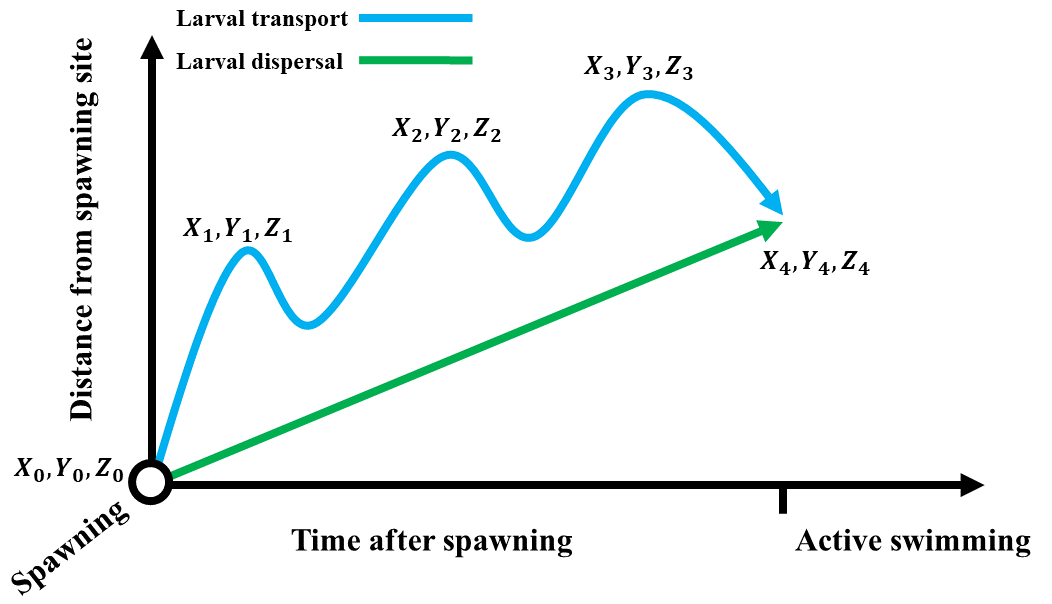
\includegraphics[width=1.0\textwidth]{figures/Chap2LarvalTransport.png}
	\centering
	\caption{Schematic representation of larval transport and larval dispersal processes. Note that the sum of the larval transport distance is greater than the dispersal distance. All locations ($X_{n},Y_{n},Z_{n}$) are pelagic.}
	\label{Chap2LarvalTransport}
\end{figure}

During larval transport, organisms are dragged by currents and depend on environmental conditions to survive, whether temperature and/or food \citep{NocrShaw1984}, and currents may allow larvae to match their food source location \citep{CuryRoy1989}. It is in this context that larval drift models, which allow tracking the trajectory of eggs and larvae through a virtual environment, are a fundamental tool for understanding the transport patterns of different species. However, before interpret modelling results it is recommended to perform a sensitivity analysis to test the robustness of these results \citep{PeckHufn2012,SimoSieg2013}. Sensitivity analysis can be understood as the manner in which model behaviour depends on model parametrization or as the variation of the response variable as a function of a change in a model parameter \citep{Hamb1994,Inga2008}. In larval drift models, results may be sensitive to the number of released particles \citep{SimoSieg2013}, to lethal temperature \citep{BrocLett2008}, to wind frequency forcing \citep{FlorTam2019}, to the spatial resolution of the forcing currents \citep{GaraKapl2014}, etc. Here we will also focus our sensitivity analysis on spatial resolution.\\

\clearpage

\section{Methods}\label{Chap2Meth}

An individual-based model (IBM) simulates populations and communities by following individuals and their properties \citep{DeanGrim2014}. As a base, this IBM, that we will use from here on, is a lagrangian tool called \href{https://ichthyop.org/}{Ichthyop} – Lagrangian tool for simulating ichthyoplankton dynamics, version 3.2 \citep{LettVerl2008}. In general, a protocol designed for this type of IBM approach will be followed \citep{GrimBerg2006,GrimBerg2010}. In the following chapters, the complexity of the model will be increased by adding specific modules for new processes.\\

\subsection{Purpose}\label{Chap2MethPurp}

To evaluate the impact of spatial resolution, bathymetry and coastline behaviour on transport and retention patterns of generic particles in the coastal zone off Peru.\\

\subsection{Entities and state variables}\label{Chap2MethEnti}

The model included two types of entities: the environment and the individuals (virtual particles). The environment was represented by stored hydrodynamic simulations from the Coastal and Regional Ocean COmmunity model (\href{https://www.croco-ocean.org/}{CROCO}, \cite{HiltAucl2020,ShchMcwi2005}) providing the forcing state variables: ocean current velocities ($ms^{-1}$), over the NHCS. Individuals were characterized by the following state variables: age ($d$), location in 3D (longitude, latitude and depth).\\

Fig. \ref{Chap2SpawningZone} xshows the three different CROCO configurations with contrasted grid size and bathymetry were used, in order to evaluate the model sensitivity to hydrodynamic resolution (Table \ref{TabSimus}). The first configuration (D01) extends from 22 °S to 5 °N in latitude and from 96 °W to 70 °W in longitude, with a horizontal resolution of $\sim$10 km and 32 vertical levels. The bathymetry comes from the STRM30 dataset \citep{BeckSand2009}. It was interpolated on the model grid and smoothed in order to reduce errors in the horizontal pressure gradient. The second configuration (D02) extends from 20 ºS to 5 ºS with a horizontal resolution of $\sim$2 km and 42 vertical levels. The D02 domain is embedded in the D01 domain, through an offline nesting procedure (``roms2roms''; \cite{MasoMole2010}). We used two different bathymetries for the D02 domain: one interpolated from the D01 bathymetry (i.e., similar to the D01 bathymetry) and one interpolated directly from the STRM30 dataset. Note that consequently the former is smoother than the latter, so in the following we call them D02s and D02r, respectively.\\

\begin{figure}[ht]
	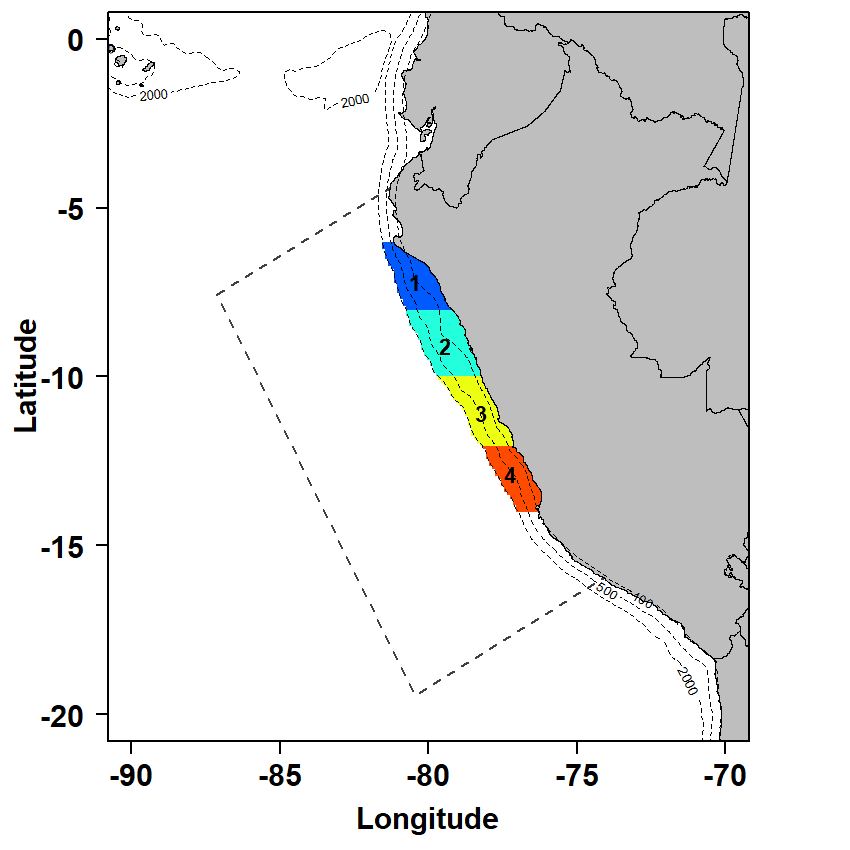
\includegraphics[width=1.0\textwidth]{figures/Chap2SpawningZone.png}
	\centering
	\caption{Domain of IBM model study area at 10 km of spatial resolution (D01). Dotted rectangle represents the nested model domains (D02s, D02s) at 2 km resolution used for spatial resolution test. Spawning areas (1 to 4) are every 2 degrees of latitude between 6º – 14º S. Three isobaths (100 m, 500 m and 2000 m) are shown.}
	\label{Chap2SpawningZone}
\end{figure}

%\begin{landscape}
\begin{table}
\centering
\begin{tabular}{c|c|c|c}
\hline
                           & \textbf{Sim 1} & \textbf{Sim 2}          & \textbf{Sim 3} \\
\hline
Configuration domain       & D01            & D02s                    & D02r           \\
Bathymetry                 & STRM30         & Interpolated from Sim 1 & STRM30         \\
Forcing type               & Physical       & Physical                & Physical       \\
Horizontal grid resolution & 10 km          & 2 km                    & 2 km           \\
CROCO configuration        & 22ºS to 5ºN    & 20ºS to 5ºS             & 20ºS to 5ºS    \\
Latitudinal spawning range & 6ºS - 14ºS     & 6ºS - 14ºS              & 6ºS - 14ºS     \\
Coastline behavior &
  \begin{tabular}[c]{@{}c@{}}beaching,\\ bouncing,\\ standstill\end{tabular} &
  \begin{tabular}[c]{@{}c@{}}beaching,\\ bouncing,\\ standstill\end{tabular} &
  \begin{tabular}[c]{@{}c@{}}beaching,\\ bouncing,\\ standstill\end{tabular}
\end{tabular}
\caption{Summary of simulations in Chapter \ref{Chap2} performed to sensitivity analysis. This table list all parameters that differ between simulations.}
\label{TabSimus}
\end{table}
%\end{landscape}

The three configurations were used to obtain quasi-equilibrium solutions, forced by monthly climatologies (over the period 2008-2015) at their surface and lateral boundaries. They all used the same atmospheric forcing fields. The wind stress was computed from a monthly climatology of the Advanced Scatterometer (\href{https://www.ospo.noaa.gov/Products/atmosphere/ascat/}{ASCAT}, 1/4° gridded product). Other atmospheric fluxes (shortwave heat fluxes and freshwater fluxes) come from the \href{https://repository.library.noaa.gov/view/noaa/49337}{COADS} monthly climatology \citep{DasiYoun1994}. Model sea surface temperature (SST) was restored to observed climatological monthly SST derived from the merged multi-sensor OSTIA product \citep{DonlMart2012} following the methodology of \citep{BarnSief1995}. Open boundary conditions for the D01 domain were derived from a monthly climatology of the \href{https://www.mercator-ocean.eu/en/ocean-science/glorys/}{GLORYS2V4} reanalysis (1/4° horizontal resolution; \citep{FerrPare2012}) for temperature, salinity, zonal and meridional current velocity components and sea-level height. Climatological simulations were run for 10 years, the first 4 years being considered as a spin-up. In the present study, the last three years were used to force Ichthyop.\\

\subsection{Process overview and scheduling}\label{Chap2MethProc}

Virtual individuals were released in the physical environment according to a determined spatial (area, depth and bathymetry) and temporal (month and frequency) releasing strategy that constituted the initial conditions (section 2.2.5). For each time step (2 hours) each egg or larva was passively transported by the 3D current fields and was then tested for recruitment.\\

\subsection{Design concepts}\label{Chap2MethDesi}

\begin{itemize}

\item Stochasticity: Individuals were initially randomly distributed over the Peruvian continental shelf. We chose the number of individuals released (5 000) such that the variability of simulated recruitment between three replicates of the same simulation was negligible.\\

\item Coastline behavior: One of the utilities of Ichthyop is the option to use different response configurations of a particle when faced with the decision of what to do when it touches the land boundary (coastline). We tested three types of coastline behaviors: 1) \textbf{BEACHING}: Ichthyop does move the particle inland but ``kill'' it. From now onward the particle is out of the simulation. 2) \textbf{BOUNCING}: the coastline acts as a billard edge and the particle will bounce as a billard ball in the events that the move would take it beyond the coastline. The particle bounces back as much as it would penetrate inland and 3) \textbf{STANDSTILL}: the particle gives up on the move that would take it inland and just wait until next time step for trying another move.\\

\item Observation: After 30 days of drift, each particle was tested to see if it was within the continental shelf and was considered ``retained'' or ``non-retained''.\\

\end{itemize}

\subsection{Initialization}\label{Chap2MethInit}

In each simulation, individuals were released randomly along the coastal release area each month at days 1, 10 and 20, during the three climatological years used.\\

Release area (Fig. \ref{Chap2SpawningZone}) was defined between latitudes 6°S and 14°S, depths 0 m to 45 m and from the coast to bathymetry contour 2000 m. This area was further splitted into different subdomains for the simulations post-processing and analysis (released depth ranges 0-15 m, 15-30 m and 30-45 m; cross-shore extension delimited by isobaths 0-100 m, 100-500 m, 500-2000 m).\\

\subsection{Sub-models}\label{Chap2MethSubMod}

\begin{itemize}

\item Transport: To simulate particle transport, virtual individuals were advected using a trilinear interpolation scheme of the velocity fields derived from CROCO, in time and space, and using a forward Euler numerical scheme with horizontal diffusion following \cite{PeliMarc2007}.\\

\item Retention: We considered one criterion for retention, hereafter referred to as the age-criterion. An individual was considered as retained if it was within the coastal zone (offshore limit: the 2000 m isobath) at age 30 days.\\

\end{itemize}

\subsection{Simulations and sensitivity analysis}\label{Chap2MethSimSens}

From this chapter onwards, each drift simulation will be listed under the name ``\textbf{sim}'', for example, in the text, saying ``sim 1'', will be equivalent to saying ``simulation 1''. Details of each simulation will be detailed in a table in its corresponding chapter.\\

Three simulations were performed in order to explore the model sensitivity to different environmental forcing fields (Table \ref{TabSimus}). In order to fit the spatial extent of the 2 km grid, individuals release was constrained in the coastal area between 6 ºS and 14 ºS (Fig. \ref{Chap2SpawningZone}, dotted box) for all three simulations. Larval retention was calculated at 30 days.\\

\clearpage

\section{Results}\label{Chap2Resu}

Globally, simulation 1 (D01), simulation 2 (D02s) and simulation 3 (D02r) showed no significant differences (Fig. \ref{Chap2Recruitment3bars}). As all simulations were run with interannual forcing, no differences in retention rates were observed in the 3 years of simulation and were also not impacted by the frequency of release (not shown).\\

\begin{figure}[ht]
	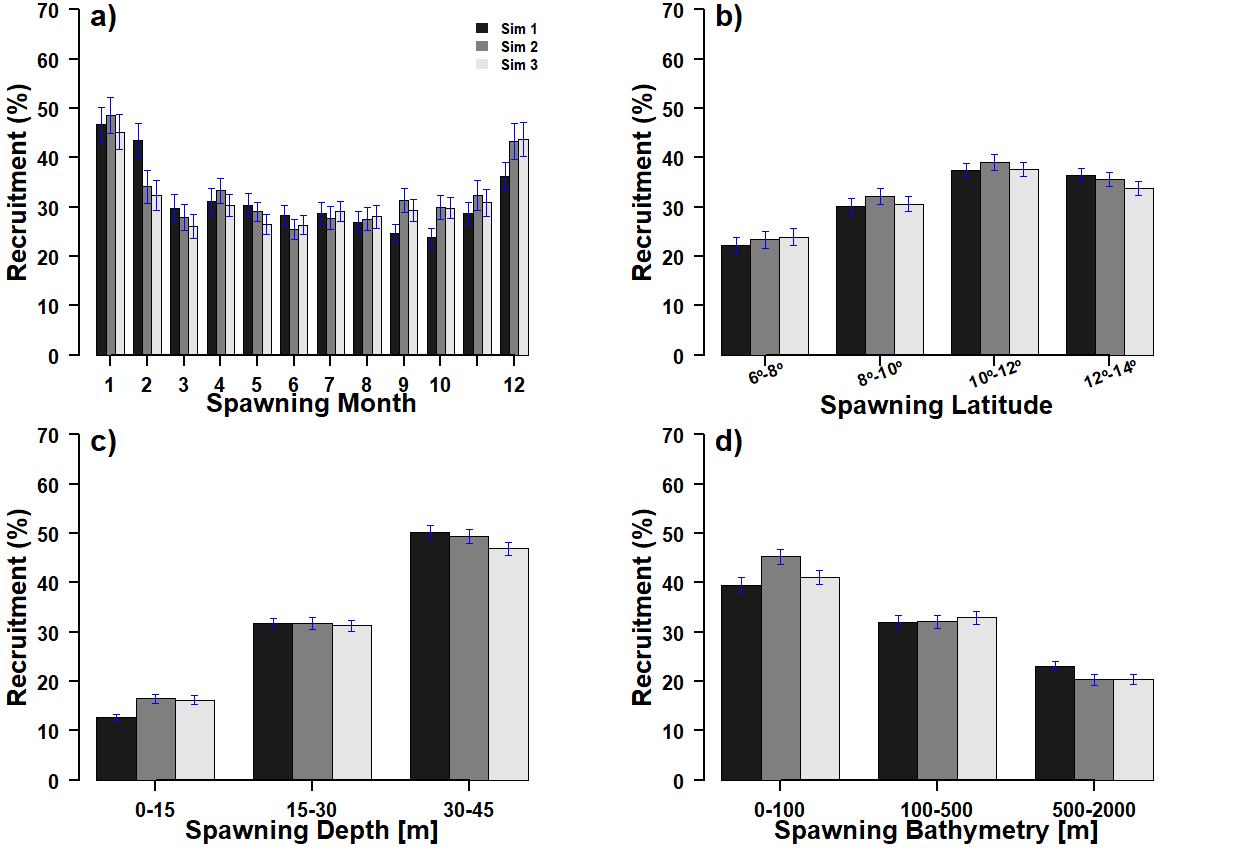
\includegraphics[width=1.0\textwidth]{figures/Chap2Recruitment3bars.png}
	\centering
	\caption{Percentage of recruited larvae of Peruvian anchovy obtained for different (a) spawning months, (b) spawning latitudes, (c) spawning depths, and (d) isobaths delimiting spawning areas horizontally, for three simulations using forcing fields at different spatial resolution (Sim 1 in black, Sim 2 in dark grey, Sim 3 in light gray; see Table \ref{TabSimus} for details on simulations characteristics). Blue arrows represent confidence interval (95 \%).}
	\label{Chap2Recruitment3bars}
\end{figure}

Since spatial resolution is not a factor that significantly affected retention rates, the results of the 3 simulations were combined and an ANOVA (Table \ref{TabAnovaSimus}) was applied to evaluate which of the other factors (release month, release latitude, release depth and release bathymetry) had the greatest impact. Release depth explained 30.11 \% of the variance and showed a direct relationship between release depth and retention rate, with higher values when the particles were released deeper (30 - 45 m) and lower values when they were released near the surface (0 - 15 m) (Fig. \ref{Chap2Recruitment3bars}c). Release bathymetry explained 12.95 \% of the variance, with the highest retention rates in the area closest to the coast (0 - 100 m) than those released offshore (100 - 500 m, 500 - 2000 m) (Fig. \ref{Chap2Recruitment3bars}d). Release month explained only 5.56 \% of the variance and showed seasonal variability with the summer months having the highest retention rate (Fig. \ref{Chap2Recruitment3bars}a). Finally, release latitude explained 4.58 \% of the variance and the zone between 10 - 12 ºS was the major latitudinal retention zone (Fig. \ref{Chap2Recruitment3bars}b).\\

\begin{landscape}
\begin{table}
\begin{tabular}{c|r|r|r|r|r|r}
\hline
 &
  \multicolumn{1}{c|}{\textbf{Df}} &
  \multicolumn{1}{c|}{\textbf{Sum Sq}} &
  \multicolumn{1}{c|}{\textbf{Mean Sq}} &
  \multicolumn{1}{c|}{\textbf{F value}} &
  \multicolumn{1}{c|}{\textbf{Pr (\textgreater{}F)}} &
  \multicolumn{1}{c}{\textbf{\% Exp}} \\
\hline
Year                  & 2     & 445.15     & 222.57     & 1.67    & 0.1883824  & 0.006  \\
Month                 & 11    & 402974.67  & 36634.06   & 274.79  & 0          & 5.567  \\
Depth                 & 2     & 2179965.33 & 1089982.67 & 8175.98 & 0          & 30.114 \\
Bathymetry            & 2     & 937366.31  & 468683.15  & 3515.60 & 0          & 12.949 \\
Latitude              & 3     & 331526.69  & 110508.90  & 828.93  & 0          & 4.580  \\
Year x Month          & 22    & 10599.92   & 481.81     & 3.61    & 2.11E-08   & 0.146  \\
Year x Depth          & 4     & 645.77     & 161.44     & 1.21    & 0.30375276 & 0.009  \\
Year x Bathymetry     & 4     & 2448.21    & 612.05     & 4.59    & 0.0010536  & 0.034  \\
Year x Latitude       & 6     & 17687.31   & 2947.88    & 22.11   & 5.02E-26   & 0.244  \\
Month x Depth         & 22    & 795678.29  & 36167.20   & 271.29  & 0          & 10.991 \\
Month x Bathymetry    & 22    & 111246.09  & 5056.64    & 37.93   & 2.63E-156  & 1.537  \\
Month x Latitude      & 33    & 526941.97  & 15967.94   & 119.78  & 0          & 7.279  \\
Depth x Bathymetry    & 4     & 49715.80   & 12428.95   & 93.23   & 3.67E-78   & 0.687  \\
Depth x Latitude      & 6     & 54521.66   & 9086.94    & 68.16   & 1.07E-83   & 0.753  \\
Bathymetry x Latitude & 6     & 282366.47  & 47061.08   & 353.01  & 0          & 3.901  \\
Residuals             & 11514 & 1534992.47 & 133.32     & -       & -          & 21.204
\end{tabular}
\caption{ANOVA of retention rates for simulation 1 (D01), simulation 2 (D02s) and simulation 3 (D02r) combined.}
\label{TabAnovaSimus}
\end{table}
\end{landscape}

Release depth had the highest and most significant effect on all 3 simulations affecting the seasonal pattern (Fig. \ref{Chap2Recruitment3sim3depth}). Particles released near the surface (0-15 m, Fig. \ref{Chap2Recruitment3sim3depth} a, d, g) showed a seasonal pattern favoring retention in the winter months, while this pattern reverses as release depth increases (15 - 30 m, Fig. \ref{Chap2Recruitment3sim3depth} b, e, h; 30 - 45 m, c, f, i).\\

\begin{figure}[ht]
	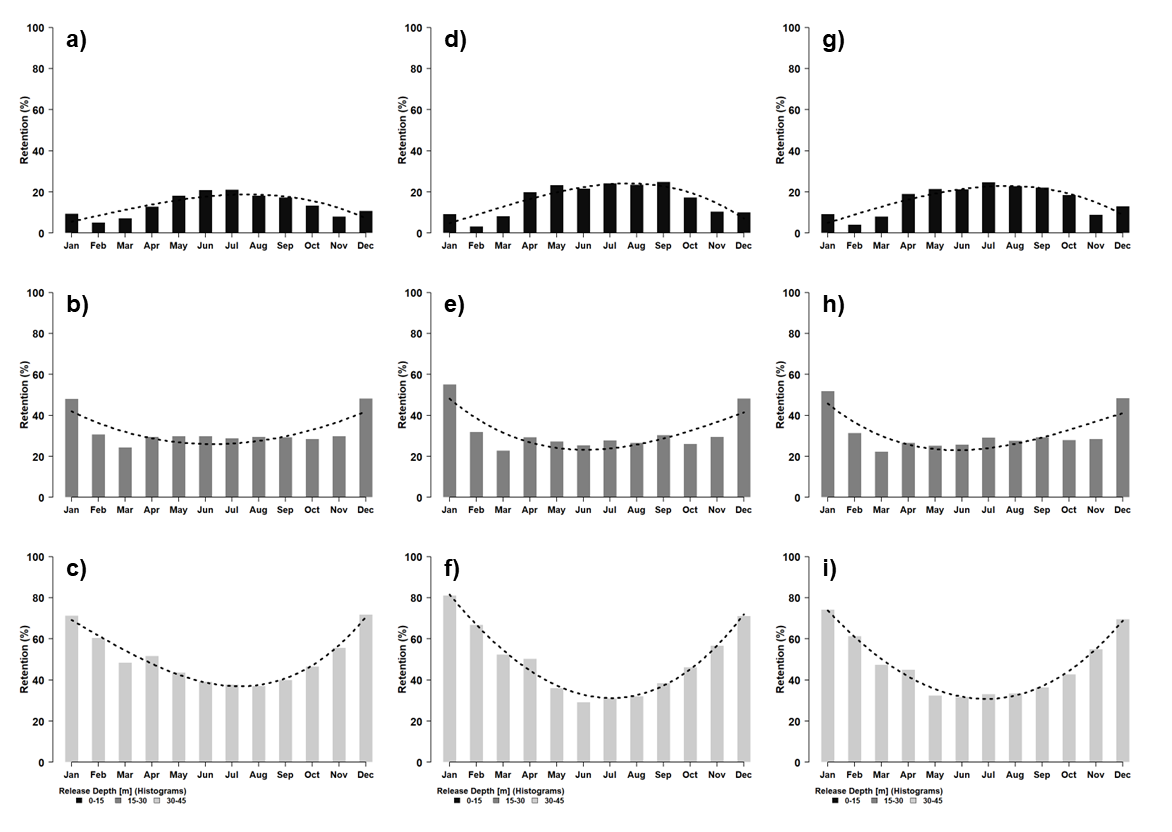
\includegraphics[width=1.0\textwidth]{figures/Chap2Recruitment3sim3depth.png}
	\centering
	\caption{Particle retention rates off Peru using 3 different physical forcing configurations (D01, a,b,c; D02s, d,e,f; D02r, g,h,i) and three release depths (0 – 15 m, 15 - 30 m and 30 - 45 m).}
	\label{Chap2Recruitment3sim3depth}
\end{figure}

Fig. \ref{Chap2SpatialVariation} showed that retention rates between 10\textdegree S - 12\textdegree S remained constant throughout the year in the 3 simulations. The northern zone between 6\textdegree S - 10\textdegree S showed seasonal variability with higher retention values in summer and accented values in January and February in simulation 2 (D02s).\\

\begin{figure}[ht]
	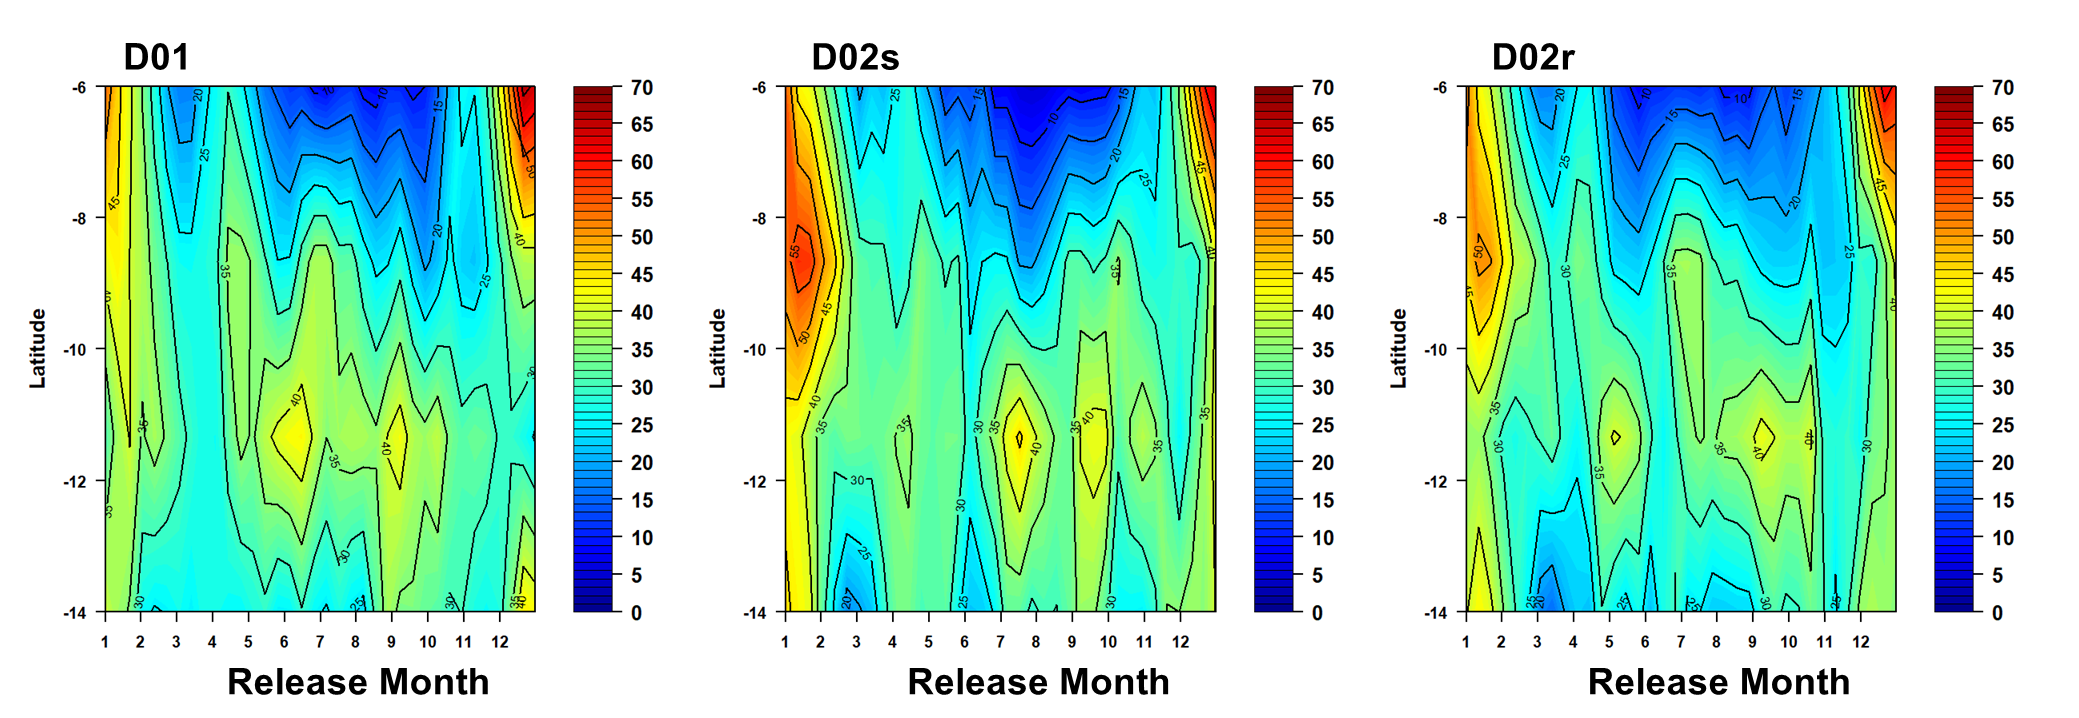
\includegraphics[width=1.0\textwidth]{figures/Chap2SpatialVariation.png}
	\centering
	\caption{Spatial variation of retention rates for simulation 1 (D01), simulation 2 (D02s) and simulation 3 (D02r).}
	\label{Chap2SpatialVariation}
\end{figure}

Fig. \ref{Chap2CoastlineBehavior} describes the interaction between release bathymetry and coastline behavior. Only in the area closest to the coast (0 - 100 m of bathymetry) the beaching coastline behavior had a significant effect in simulation 1 (D01), simulation 2 (D02s) and simulation 3 (D02r). The other 2 coastlines behaviours had not an important effect.\\

\begin{figure}[ht]
	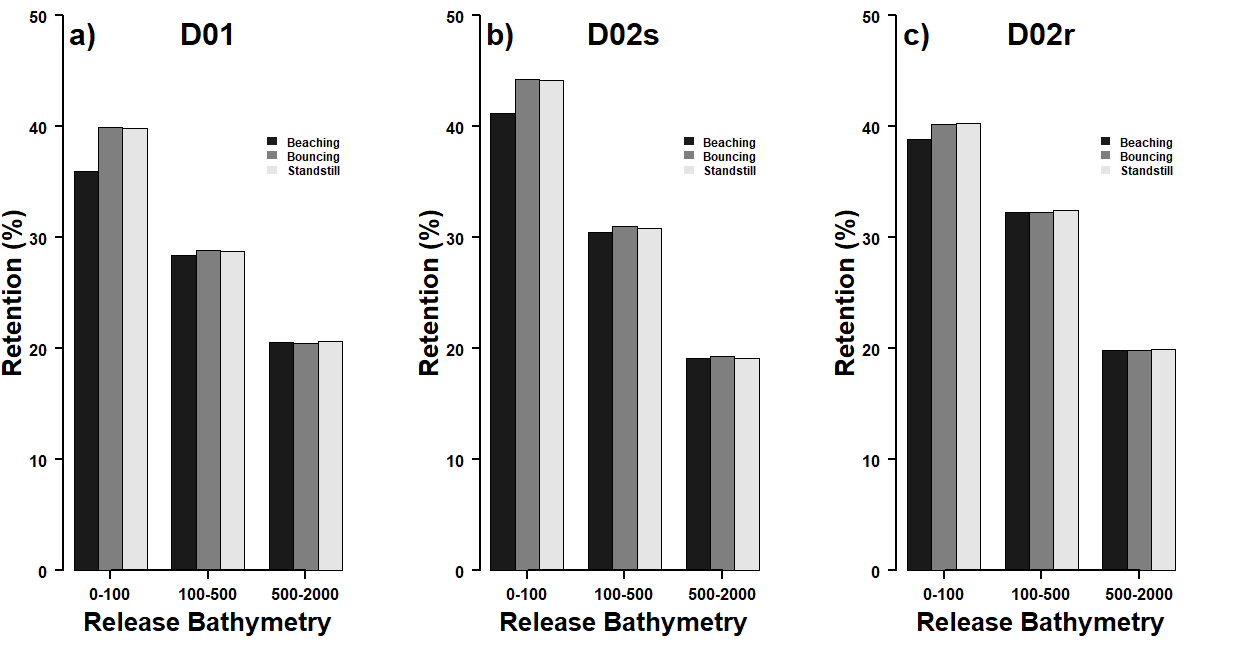
\includegraphics[width=1.0\textwidth]{figures/Chap2CoastlineBehavior.png}
	\centering
	\caption{Barplots of retention rates as a function of coastline behavior and release bathymetry for simulation 1 (D01), simulation 2 (D02s) and simulation 3 (D02r).}
	\label{Chap2CoastlineBehavior}
\end{figure}

\clearpage

\section{Discussion}\label{Chap2Disc}

A sensitivity analysis to spatial resolution, bathymetry and coastline behavior was applied to the retention rates off Peru using Ichthyop model, a powerfull Lagrangian tool \citep{LettVerl2008}. This tool allowed us to track virtual particles in a 3D environment and to know the location of each particle at each time step.\\

The fact that there was no significant difference between simulation 1 (D01), simulation 2 (D02s) and simulation 3 (D02r) strengthen the conclusions found by \citep{BrocLett2008} who used a spatial resolution forcing only slightly greater than 10 km, despite their study had a wider latitudinal range (2º - 20º S) than the one used in this chapter (6º - 14º S). \cite{BrocLett2008} also found that release depth is the most important factor (22.7 \% of explained variance) although in a smaller proportion than in the present chapter (30.11 \%). However, \cite{BrocLett2008} found that the next most important factors were release latitude (7.2 \%) and then release bathymetry (3.9 \%), in contrast to the present chapter in which release latitude (4.58 \%) was less important than release bathymetry (12.95 \%). Concerning the release bathymetry, finding a higher value of percentage of variance explanation in this chapter compared to \cite{BrocLett2008}, could be due to the topographic sources \citep{SmitSand1997} used by them and the one used in the present chapter \citep{BeckSand2009} to represent the bathymetry, which could provide a better description of the seafloor and affect circulation and retention structures also affecting retention rates as \cite{RojaLand2014} reported.\\

\cite{LettPenv2007} applied Lagrangian simulation experiments to evaluate the processes of enrichment, retention and concentration proposed as the mechanisms that favor the recruitment of marine species \citep{Baku1998, Baku2010}. \cite{LettPenv2007} showed that after 20 days of drifting, the zones of highest retention were located between grade 10\textdegree S - 14\textdegree S, similar to our results in the 3 simulations, values that were constant throughout the year in this latitudinal range, even though retention was calculated after 30 days of drift. \cite{LettPenv2007} also showed a general seasonal pattern with the summer months favoring retention as well as in this chapter, however, we can now know that retention is highly dependent on initial depth (release depth), in agreement with \cite{BrocLett2008}, therefore, the larval retention of any species will depend on its spawning depth or its vertical behaviour \citep{OspiPara2012}.\\

A spatial resolution analysis was applied in the Humboldt ecosystem for one mollusk species \citep{GaraKapl2014}. Between 3 km and 7.5 km hydrodynamic forcings, no difference in dispersion distance was observed, however, both experiments also demonstrated that the closer to coast, the greater the success of the individuals, in this case called larval settlement (and retention in this chapter). It should be noted that they used much longer drift times (80 days and 140 days).\\

Something that was not evaluated in this work was the effect of wind forcing frequency (monthly winds and daily winds) at high resolution (2 km, D02), which results in increased retention rates while maintaining patters patterns although this was applied in very coastal and small areas at the level of a bay \citep{FlorTam2019}.\\

This could have implications when we use different coastline behaviors, as demonstrated in this chapter, in which only beaching behavior in areas very close to the coast (0 - 100 m) had significant impacts on retention rates, although did not have a major impact at level of the continental shelf off Peru, could have a significant effect if we study problems such as oil spills or accumulation of microplastics on the coast \citep{AtwoFalc2019,LopeNajj2021}.\\

Finally, we can conclude that to work on \textit{E. ringens} recruitment simulations, in order to save computational time and energy, we can continue with a spatial resolution of 10 km. In addition, it is recommended to use the coastal behaviour called standstill, since for the purposes of our research it will not significantly affect near-shore particle transport.\\

\clearpage
\chapter{Influence of combined temperature and food availability on Peruvian anchovy (\textit{Engraulis ringens}) early life stages in the northern Humboldt Current system:\\A modelling approach}\label{Chap3}

\clearpage
This chapter is based on the following published scientific paper \citep{FlorLett2023} \textbf{\textit{Influence of combined temperature and food availability on Peruvian anchovy (\gls{ringens}) early life stages in the northern Humboldt Current system: A modelling approach.}}\\

Available at: \href{https://www.sciencedirect.com/science/article/abs/pii/S0079661123000770}{Progress in Oceanography}.

\clearpage
\section*{Abstract}

In the \acrfull{nhcs}, the Peruvian anchovy (\textit{\gls{ringens}}) constitutes the bulk of landings and has a significant socioeconomic contribution. Understanding the impact of environment on the early-life stages of anchovy and further population dynamics remains challenging. Climate variability at a variety of scales modulates currents velocity, temperature and food availability, impacting early-life stages drift, growth and survival. In order to investigate these impacts, we developed \gls{ich-deb}, an individual-based model including larval retention processes and a \acrfull{deb} bioenergetic module for larval growth. We evaluated the impact of the following biological processes on simulated larval recruitment patterns: i) a minimum size-criterion (2 $cm$), compared to a minimum age-criterion (30 $days$), to be considered as recruited, ii) the upper larval thermal limit tolerance of the species, for which lab experiments are lacking, and iii) a constant larval mortality rate. Simulated larval retention patterns was highest when spawning occurred in the superficial layer (0 - 15 $m$) in austral winter and in the deepest considered layer (30 - 45 $m$) in summer. Coupling with the DEB model produced contrasted growth patterns on the continental shelf with a strong month-latitude interaction. Larval recruitment was strongest from 6\textdegree  to 10\textdegree $S$ in austral summer, largely contributing to the average seasonal pattern. Depending on the temperature correction function tested with the bioenergetic module, simulated larval recruitment could also be strong in the northernmost zone (2\textdegree - 4\textdegree $S$), an area not known for abundant anchovy populations, which suggests a possible thermal growth limitation. Finally, sensitivity tests performed on larval growth limitation by food suggested a deficiency in food supply in the southernmost zone (18\textdegree - 20\textdegree $S$).\\

Keywords: Ichthyop-DEB model, early life stages survival, Peruvian anchovy, larval drift, larval growth

\clearpage
\section{Introduction}\label{Chap3Intro}

The \acrfull{nhcs} currently produces more fish catch per unit area than any other marine ecosystem \citep{BakuWeek2008,ChavBert2008} despite not having the largest primary productivity \citep{ChavMess2009,ChecAsch2017}. In the \acrshort{nhcs}, the Peruvian anchovy (\textit{\gls{ringens}}) is a highly prolific species ($\sim$15 000 $eggs/batch$) that reaches its sexual maturity at the age of one year. The anchovy spawns mainly in the coastal zone close to surface \citep{GutiSwar2007,GutiRami2008}. Early life stages are taking advantage of the exceptional continental shelf nursery area thanks to the high productivity from the upwelling zone, which contribute to make \textit{\gls{ringens}} the most abundant species, supporting the world largest mono-specific fishery \citep{FreoMull2003,AlheNiqu2004,GutiAkes2016,ChecAsch2017,FAO2020}. \textit{\gls{ringens}} fishery is managed based on scientific monitoring of population indicators \citep{Ayon2000,GutiSwar2007}, but the link between environmental variability and anchovy recruitment, and thereby biomass of the adult population, is still unclear.\\

Modelling studies have been conducted to understand the hydrodynamics of the \acrshort{nhcs} \citep{PenvEche2005,ColaMcwi2012}, its interannual variability \citep{ColaCape2008,EspiEche2017}, its potential changes under future climate scenarios \citep{OerdCola2015,EcheGeva2020}, and the seasonal cycle and intraseasonal variability of surface chlorophyll \citep{EcheAumo2008,EcheAlbe2014}. These works provided the physical and biogeochemical basis for ecological studies in the \acrshort{nhcs}, from testing Bakun's triad hypothesis \citep{Baku1998} for small pelagic fish recruitment and early life stages survival \citep{LettPenv2007} to simulating Peruvian anchovy recruitment depending on environmental conditions \citep{BrocLett2008,BrocCola2009,BrocLett2011,BrocEche2013,XuChai2013,XuRose2015}.\\

The first anchovy larval drift modelling study conducted in the \acrshort{nhcs} found similarities between simulated anchovy larval near surface retention over the continental shelf and observed egg distribution \citep{BrocLett2008}. This results suggests a reproductive strategy of the Peruvian anchovy adapted to maximize reproduction success, a pattern also found in other Eastern Boundary Upwelling Systems \citep{BrocCola2009}. Later, \cite{BrocEche2013} used a physical-biogeochemical model to evaluate the effect of currents and productivity on nursery areas reduction due to climate change, and found a negative effect on Peruvian anchovy early life stages survival. However, the effects of temperature and food availability on larval growth and survival were not directly taken into account and coastal retention was evaluated using a constant \acrfull{pld} of 30 $days$ (recruitment age-criterion). \cite{XuChai2013} applied a 3D full life cycle model to the Peruvian anchovy over the period 1991 - 2007 using a bioenergetic growth model, with a 5 $cm$ limit for the successful recruitment of individuals (recruitment size-criterion). They obtained an increased age at recruitment in 1998 (El Ni\~{n}o conditions) as well as a notable decrease in individuals’ survival. Then, \cite{XuRose2015} underlined the importance of spatial variability in environmental conditions of the \acrshort{nhcs} and thereby on simulated recruitment of Peruvian anchovy.\\

Despite these previous works, the question of the relative contribution of the two main \textit{\gls{ringens}} spawning seasons to the over-all recruitment remain an open debate \citep{WalsWhit1980,PerePena2011}. Here we tested the hypothesis that the higher food availability combined with warmer condition in summer could contribute to better growth conditions in this season, and compensate for the lower retention pattern previously predicted in the surface layer. Such hypothesis would imply the summer spawning to be the main contribution to recruitment, which could have consequences for \textit{\gls{ringens}} fisheries management in Peru. In order test this hypothesis, we developed \gls{ich-deb}, an \acrfull{ibm} including larval retention processes \citep{LettVerl2008} and a \acrfull{deb} \citep{Kooi2009} bioenergetic module for larval growth. Using this tool, we assessed the effect of hydrodynamic simulations horizontal resolution on simulated larval retention patterns using a recruitment age-criterion of 30 $days$. Then, we evaluated the impact of the following biological processes on simulated larval recruitment: i) a minimum size-criterion (2 $cm$), as opposed to a minimum age-criterion (30 $days$), to be considered as recruited, ii) the upper larval thermal limit tolerance of the species, for which lab experiments are lacking, and iii) a constant larval mortality rate.

\clearpage
\section{Methods}\label{Chap3Meth}
The methodology of this chapter is similar to that applied in Chapter \ref{Chap2}, but will include the description and implementation of a \acrshort{deb} growth model and only $D01$ will be used as forcing, since the spatial resolution did not show significant effects when studying larval
retention in Chapter \ref{Chap2}, in addition we extended the spawning zone domain from 6\textdegree -14\textdegree $S$ to 2\textdegree -20\textdegree $S$ and the mesozooplankton field from CROCO-PISCES model was used as input for the growth model. Simulations 4 to 8 listed in Table \ref{Chap3TabSimus} were performed with climatological forcings, and the same \gls{ich-deb} (Fig. \ref{Chap3Ichthyop-DEB}) configuration was used to run 2 extra simulations (9-10) with interannual forcing from 1980 to 2000 to evaluate the effect of El Ni\~{n}o, for Case 1 and Case 2 curve of temperature correction.\\

\begin{figure}[ht]
	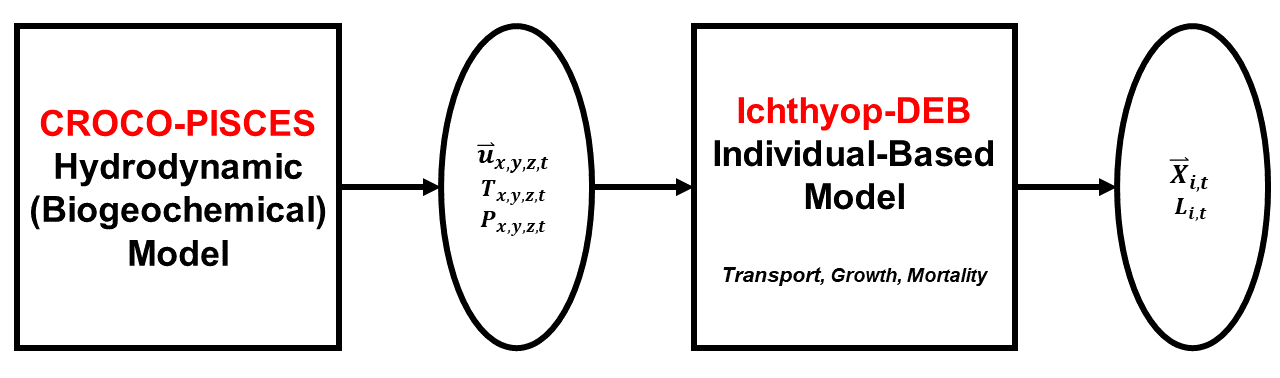
\includegraphics[width=1.0\textwidth]{figures/Chap3Ichthyop-DEB.png}
	\centering
	\caption{Representative flow diagram of the Ichthyop-DEB model and its hydrodynamic-biogeochemical forcing using CROCO-PISCES.}
	\label{Chap3Ichthyop-DEB}
\end{figure}

\subsection{Design concepts}

\begin{itemize}

\item Observation: A spatio-temporal recruitment index was computed for each simulation and compared with egg presence observational data. Three recruitment criterions were tested, either based on 30-day retention over the continental shelf (\gls{cri1}), retention until the larval length reach 2 $cm$ (\gls{cri2}) and mortality-weighted larval worth until the larval length reach 2 $cm$ (\gls{cri3}). Standard length of a larva used for criterion \gls{cri2} and \gls{cri3} relates to its structural volume as follows:\\

\begin{equation}
	L_{w} = \frac
				{V^{1/3}}
				{\delta_{M}}
	\label{L_W}
\end{equation}\\

where $L_{w}$ is the physical standard length ($cm$), $V$ is the structural volume ($cm^3$) 
and $\delta_{M}$ is a shape coefficient.\\

\end{itemize}

\subsection{Initialization}
In each simulation, individuals were released randomly along the coastal spawning area (Fig. \ref{Chap3SpawningZone}) each month at days 1, 10 and 20, during the three climatological years used. The coastal spawning area was defined as the volume of water between latitudes 2\textdegree $S$ and 20\textdegree $S$, depth range [0 - 45 $m$] and from the coast to isobath 2000 $m$.\\

The initial values of the bioenergetic variables for each individual were set as initial reserve $E0=1J$ and initial structure $V0=0.000001cm^3$. Formally, an egg is only composed of reserve but in practice a very small value for $V0$ value was needed in order to avoid division by zero in the mobilization equation. We checked that a value of $V0$ larger by one order of magnitude did not change the results.\\

\begin{figure}[ht]
	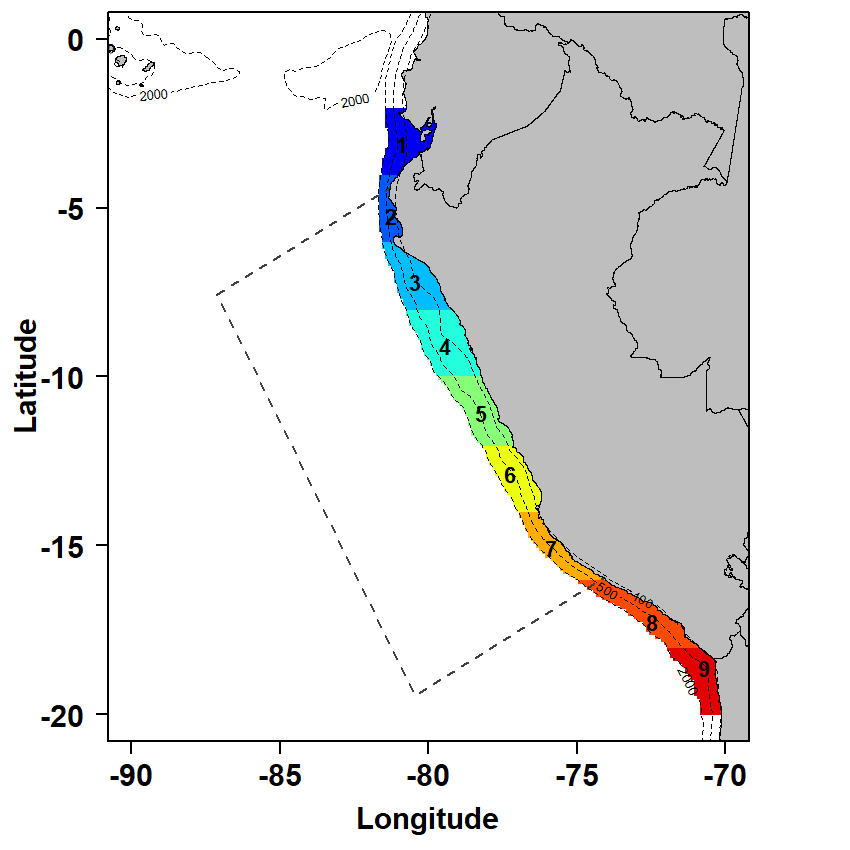
\includegraphics[width=1.0\textwidth]{figures/Chap3SpawningZone.png}
	\centering
	\caption{Model domain at 10 km of spatial resolution ($D01$). Spawning areas (1 - 9) are every 2\textdegree degrees of latitude between 2\textdegree $S$ and 20\textdegree $S$. Three isobaths (100 $m$, 500 $m$ and 2000 $m$) are shown.}
	\label{Chap3SpawningZone}
\end{figure}

\subsection{Sub-models}

\begin{itemize}

\item Growth: The \acrshort{deb} theory \citep{Kooi2009} was used to simulate the growth of larvae. It describes the acquisition and utilization of energy for metabolic processes during the complete life cycle of an organism depending on temperature ($T$) and food conditions ($f$). Here, this model was used to simulate larval growth through the description of energy reserve and body structure complexity evolution; maturation and reproduction processes were not considered. Energy assimilated from food in the environment is allocated partly to reserve for somatic maintenance ($E$), and the excess energy is used to increase the structure ($V$), i.e., physical length (see eqn. \ref{L_W}). The following system of ordinary differential equations describe the dynamics of $E$ (eqn. \ref{dEdt}) and $V$ (eqn. \ref{dVdt}).\\

Each parameter may be identified from specific observations for any species. In the absence of observations for the Peruvian anchovy (\textit{\gls{ringens}}), we used here parameters estimated for the European anchovy (\textit{\gls{encrasicolus}}, \cite{PethRoos2013}	, Table \ref{Chap3TabDEBparEncra}), a taxonomically close species that is also distributed in upwelling zones. $\left \{ \dot{p}_\mathrm{Am} \right \}$ is the surface-area-specific maximum assimilation rate, $\left [ \dot{p}_{M} \right ]$ is the specific volume-linked somatic maintenance rate, $\kappa$ is the fraction of mobilized reserve allocated to soma, ${\left [ E_{G} \right ]}$ is the volume-specific costs of structure and $\dot{p}_{C}$ (eqn. \ref{pC}) is a compound parameter corresponding to the mobilization of energy for maintenance,\\

\begin{equation}
	\dot{p}_{C} = \frac
					   {E\left ( \left [ E_{G} \right ] \frac{C_{T}\left \{ \dot{p}_\mathrm{Am} \right \}}{\left [ E_{m} \right ]} V^{-\frac{1}{3}}+\left [ \dot{p}_{M} \right ]\right )}
					   {\kappa\left ( \frac{E}{V} \right ) + \left [ E_{G} \right ]}
	\label{pC}
\end{equation}\\

where $\left[ E_{m} \right]$ is the maximum reserve density and $fC_{T}\left \{ \dot{p}_\mathrm{Am} \right \}V^{\frac{2}{3}}$ corresponds to the assimilation of energy which begins after birth, based on the following food concentration functional response (eqn. \ref{funct_response}),\\

\begin{equation}
	f = \frac{X}
			 {X+K}
    \label{funct_response}
\end{equation}\\

with $X$ the local food concentration (here meso-zooplankton fields coming from CROCO-PISCES), $K$ the half-saturation constant fixed with a value of 1.6 and $C_{T}$ a non-monotonic temperature correction factor. The parameter $C_{T}$ is defined as follows:\\

\begin{equation}
	C_{T} = exp\left ( \frac{T_{A}}{T_{1}} - \frac{T_{A}}{T} \right )
	\left ( \frac
				{1+exp\left ( \frac{T_{AL}}{T_{1}} - \frac{T_{AL}}{T_{L}} \right )
				  +exp\left ( \frac{T_{AH}}{T_{H}} - \frac{T_{AH}}{T_{1}} \right )}
				{1+exp\left ( \frac{T_{AL}}{T} - \frac{T_{AL}}{T_{L}} \right )
				  +exp\left ( \frac{T_{AH}}{T_{H}} - \frac{T_{AH}}{T} \right )}
	\right )
    \label{C_T}
\end{equation}\\

\begin{equation}
	\frac{dE}{dt} = f C_{T} \left \{ \dot{p}_\mathrm{Am} \right \} V^{\frac{2}{3}} - \dot{p}_{C}
	\label{dEdt}
\end{equation}\\

\begin{equation}
	\frac{dV}{dt} = \frac
						{\kappa \dot{p}_C - C_{T} \left [ \dot{p}_{M} \right ] V}
						{\left [ E_{G} \right ]}
	\label{dVdt}
\end{equation}\\

where $T$ is the water temperature surrounding an individual (coming from CROCO-PISCES), $T_{1}$ is the reference temperature (for which flux parameters were estimated), $T_{A}$ is the Arrhenius temperature \citep{Kooi2009} and $T_{AL}$, $T_{AH}$, $T_{L}$, $T_{H}$ are constants used to define a curved shape of the temperature correction according to temperature.\\

\item Recruitment: We considered two criteria for larval recruitment, hereafter referred to as the
age- and size-criterion, respectively. For the age-criterion (\gls{cri1}), an individual was considered
as recruited if it was within the coastal zone (offshore limit 2000 $m$ isobath) at age 30
$days$, like in the previous modelling study \citep{BrocLett2008}. For the size-criterion (\gls{cri2}), an individual was considered as recruited when it was within the coastal zone at a size larger
than 20 $mm$. The 20 $mm$ threshold was chosen because Peruvian anchovy larvae reached
an average size of 20 $mm$ at 30 $days$ \citep{CastHern2000, MoreClar2011, RiouOfel2021, OfelMoya2023}.\\

\item Mortality: We used the concept of super-individual \citep{ScheBave1995, ParrEvan2008} by assigning an initial worth of 1 to each individual, then applying a constant daily mortality rate until the age at recruitment, which we will call \gls{cri3}. The daily mortality rate was set to $0.1 d^{-1}$ as proposed for anchovies \citep{BailHoud1989, Houd2008}. The formula used to construct mortality is as follows: $(1-0.1)^{age}$, where $age$ is ``age at recruitment'', thus, individuals who recruit earlier will have a higher value than those who take longer, as shown in Fig. \ref{Chap3MortalityCurve}.

\end{itemize}

\begin{figure}[ht]
	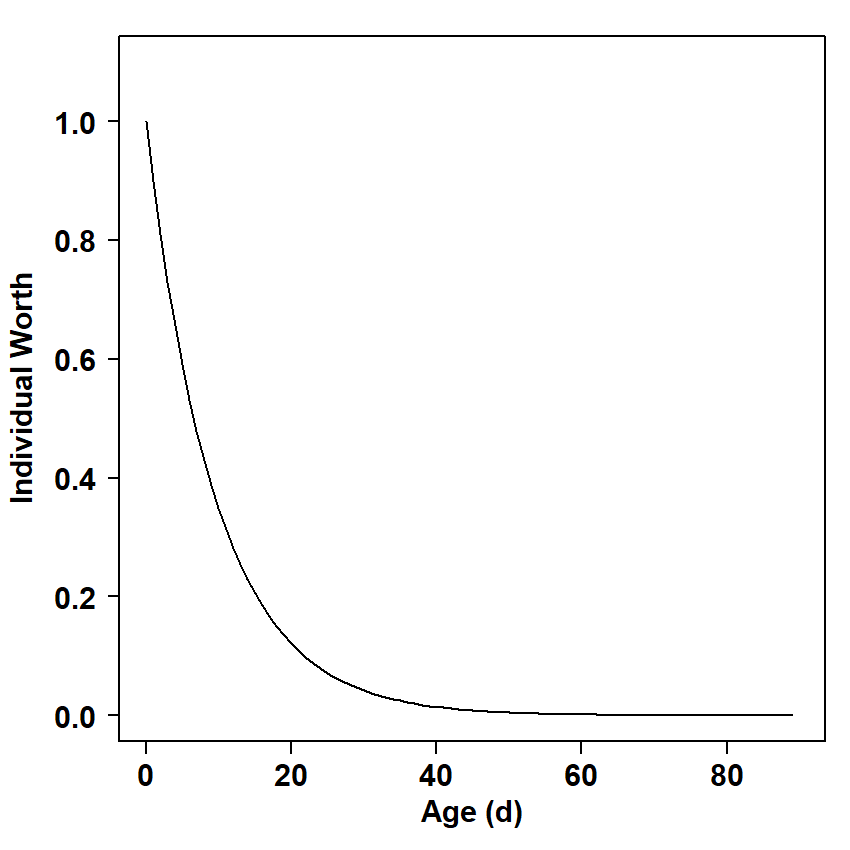
\includegraphics[width=1.0\textwidth]{figures/Chap3MortalityCurve.png}
	\centering
	\caption{The worth of an individual is a function of age, with a constant mortality rate of $0.1 d^{-1}$.}
	\label{Chap3MortalityCurve}
\end{figure}


\begin{landscape}
\begin{table}[H]
    \centering
    \caption{Summary of simulations performed to study recruitment predictions sensitivity. This table list all parameters that differ between simulations.}
    \begin{adjustbox}{width=1.0\textwidth}
    \small
    \begin{NiceTabular}{c|c|c|c|c|c|c|c}
\hline
                     &
    \textbf{$Sim 4$} &
    \textbf{$Sim 5$} &
    \textbf{$Sim 6$} &
    \textbf{$Sim 7$} &
    \textbf{$Sim 8$} &
    \textbf{$Sim 9$} &
    \textbf{$Sim 10$} \\
\hline
\makecell{Configuration \\ domain} &
	$D01$  		     &
	$D01$ 		     &
	$D01$ 			 &
	$D01$			 &
	$D01$			 &
	$D01$			 &
	$D01$			 \\
\makecell{CROCO \\ configuration}   		   &
	$22$\textdegree $S$ to $5$\textdegree $N$ &
	$22$\textdegree $S$ to $5$\textdegree $N$ &
	$22$\textdegree $S$ to $5$\textdegree $N$ &
	$22$\textdegree $S$ to $5$\textdegree $N$ &
	$22$\textdegree $S$ to $5$\textdegree $N$ &
	$22$\textdegree $S$ to $5$\textdegree $N$ &
	$22$\textdegree $S$ to $5$\textdegree $N$ \\
Forcing type &
	\makecell{Physical \& \\biogeochemical} &
	\makecell{Physical \& \\biogeochemical} &
	\makecell{Physical \& \\biogeochemical} &
	\makecell{Physical \& \\biogeochemical} &
	\makecell{Physical \& \\biogeochemical} &
	\makecell{Physical \& \\biogeochemical} &
	\makecell{Physical \& \\biogeochemical} \\
Bathymetry source &
	STRM30 &
	STRM30 &
	STRM30 &
	STRM30 &
	STRM30 &
	STRM30 &
	STRM30 \\
\makecell{Horizontal \\ grid resolution} &
	$10 km$                  &
	$10 km$                  &
	$10 km$                  &
	$10 km$                  &
	$10 km$                  &
	$10 km$                  &
	$10 km$                  \\
\makecell{Latitudinal \\ spawning range}     &
	$2$\textdegree $S$ - $20$\textdegree $S$ &
	$2$\textdegree $S$ - $20$\textdegree $S$ &
	$2$\textdegree $S$ - $20$\textdegree $S$ &
	$2$\textdegree $S$ - $20$\textdegree $S$ &
	$2$\textdegree $S$ - $20$\textdegree $S$ &
	$2$\textdegree $S$ - $20$\textdegree $S$ &
	$2$\textdegree $S$ - $20$\textdegree $S$ \\					
\makecell{Growth \\ sub-model} &
	No  &
	Yes &
	Yes &
	Yes &
	Yes &
	Yes &
	Yes \\
\makecell{Recruitment \\ criterion evaluated \tabularnote{Recruitment criterion 1: retention at 30 days; 2: retention at 20 mm; 3: retention at 20 mm with constant mortality.}}  &
	1       &
	2 and 3 &
	2 and 3 &
	2 and 3 &
	2 and 3 &
	2 and 3 &
	2 and 3 \\
Correction temperature \tabularnote{Temperature correction factor Case 1: $T_{H} = 294 K$($=21$\textdegree $C$) and $T_{AH} = 95000 K$; Case 2: $T_{H} = 297 K$($=24$\textdegree $C$) and $T_{AH} = 570000 K$} &
	-      &
	Case 1 &
	Case 2 &
	Case 1 &
	Case 2 &
	Case 1 &
	Case 2 \\
\makecell{Food half \\ saturation constant \\ ($K$)}  &
	- 	&
	1.6 &
	1.6 &
	0   &
	0   &
	1.6 &
	1.6 \\
Mortality &
	-   &
	Yes &
	Yes &
	Yes &
	Yes &
	Yes &
	Yes \\
Temporal scale  &
	Climatology &
	Climatology &
	Climatology &
	Climatology &
	Climatology &
	Interannual &
	Interannual \\
\hline
    \end{NiceTabular}
    \end{adjustbox}
    \label{Chap3TabSimus}
\end{table}
\end{landscape}



%\begin{landscape}
\begin{table}[H]
    \centering
    \caption{Parameters used for the bioenergetic model describing larval growth. These values were estimated by \cite{PethRoos2013} for \textit{\gls{encrasicolus}}, except half saturation constant ($K$), estimated for the current configuration and fixed at 1.6 $\mu mol CL^{-1}$. Comparison with data showed that these parameters allowed to reproduce \textit{\gls{ringens}} larval growth. The values of $T_{L}$, $T_{H}$, $T_{AL}$, $T_{AH}$ are detailed for Case 1 and Case 2 respectively (see Table \ref{TabSimusChap3}). Although these parameters were originally calibrated with a reference temperature of 16\textdegree $C$, in order to standardize the comparison with other species, we expressed them at 20\textdegree $C$.}
    \rowcolors{1}{white}{gris}
    \begin{adjustbox}{width=1.0\textwidth}
    \begin{tabular}{l|l|l|l}
\toprule
\multicolumn{4}{l}
	{Primary parameters (rates are at reference temperature $T_{1} = 293 K$  ($=20$\textdegree $C$)} \\
\midrule
Symbol		& 
Value		& 
Unit		& 
Definition	\\
\midrule
$L_{h}$			& 
0.28			& 
$cm$			& 
Hatch length	\\
$L_{b}$									& 
0.35									& 
$cm$									& 
Yolk-sac to feeding larva threshold		\\
$T_{A}$					& 
9800					& 
$K$						& 
Arrhenius temperature	\\
$T_{L}$						& 
279/279						& 
$K$							& 
Lower temperature boundary	\\
$T_{H}$							& 
294/297							& 
$K$								& 
Upper temperature boundary		\\
$T_{AL}$									& 
20000/20000									& 
$K$											& 
Arrhenius temperature for lower boundary	\\
$T_{AH}$										& 
95000/570000									& 
$K$												& 
Arrhenius temperature for upper boundary		\\
$K$							& 
1.6							& 
$\mu mol CL^{-1}$			& 
Half-saturation constant	\\
$\kappa_{\mathrm{x}}$						& 
0.71										&
 -											&
Fraction of food energy fixed in reserve	\\
$\left\{\dot{p}_\mathrm{Xm} \right\}$			&
516												&
$J.cm^{-2}.d^{-1}$								& 
Maximum surface-specific ingestion rate		\\
$\left[E_{m} \right]$		& 
2700						& 
$J.cm^{-3}$					& 
Maximum reserve density		\\
$\left[E_{G} \right]$				& 
4000								& 
$J.cm^{-3}$							& 
Volume-specific costs of structure	\\
$\left[\dot{p}_{M} \right]$					& 
76.22										& 
$J.cm^{-3}.d^{-1}$							& 
Volume-specific somatic maintenance rate	\\
$\kappa$																				& 
0.7																						& 
- 																						& 
\makecell[l]
	{Fraction of mobilized reserve allocated to \\ growth and somatic maintenance}	\\
\midrule
\multicolumn{4}{l}
	{Auxiliary and Compounds parameters}   \\
\midrule
Symbol		& 
Value		& 
Unit		& 
Definition	\\
\midrule
$\delta_{M}$		& 
0.152				& 
-					& 
Shape coefficient	\\
$\left \{ \dot{p}_\mathrm{Am} \right \}$								& 
$\kappa_{\mathrm{x}} $ $\left \{ \dot{p}_\mathrm{Xm} \right \}=366$	&
$J.cm^{-2}.d^{-1}$														& 
Maximum surface-area-specific assimilation rate						\\
\bottomrule
\end{tabular}
\end{adjustbox}
\label{Chap3TabDEBparEncra}
\end{table}
%\end{landscape}

\subsection{Simulations and sensitivity analysis}

Table \ref{Chap3TabSimus} shows seven simulations named from $Sim4$ to $Sim10$ performed in order
to explore the model sensitivity to different environmental forcing fields and larval growth
parameters using the $D01$ grid and the larval size threshold (20 $mm$) as a criterion for
recruitment (size-criterion). The \acrshort{deb} parameters values are given in Table \ref{Chap3TabDEBparEncra}, corresponding to \textit{\gls{encrasicolus}} \citep{PethRoos2013} but fitting \textit{\gls{ringens}} larval growth well. In order to disentangle the effects of food and temperature on growth, and ultimately on recruitment, simulations were repeated using a half saturation parameter either null, i.e., $f = 1$ (no food limitation) or calculated such that $f = 0.5$ for the average meso-zooplankton concentration over the continental shelf off Peru with a half saturation constant of $K = 1.6$. To contrast the effect of temperature on growth, we used two different shapes for the curve of the energy fluxes temperature correction ($C_{T}$; Fig. \ref{Chap3CT_curves}). In both cases, $C_{T}$ dropped to very low values for temperature higher than $25$\textdegree $C$ but in the first case the maximum value of $C_{T}$ was at $19$\textdegree $C$ and then it dropped slowly (hereafter referred to as ``Case 1'') whereas in the second case the maximum was at 23 \textdegree C and then it dropped quickly (hereafter referred to as ``Case 2''). These temperature thresholds were chosen to fit \textit{\gls{ringens}} distribution in Peru \citep{CastPena2022}. Two additional simulations were conducted under the same configuration as cases 1 and 2, with an interannual forcing. The objective was to explore recruitment on a different time scale than the climatological one. All simulations lasted 90 days, a value found from preliminary simulations as long enough for the slowest growing individuals to reach the recruitment size. Larval retention at 30 days (age criterion, $Sim 4$) was also compared with the size-criterion in all four simulations ($Sim 5$, $Sim 6$, $Sim 7$ and $Sim 8$). In order to quantify the variation of results between simulations with ($Sim 5$, $Sim 6$) and without ($Sim 7$, $Sim 8$) food limitation, we calculated the percentage of variation, e.g. ($\frac{Sim 7-Sim 5}{Sim 5*100}$)

\begin{figure}[ht]
	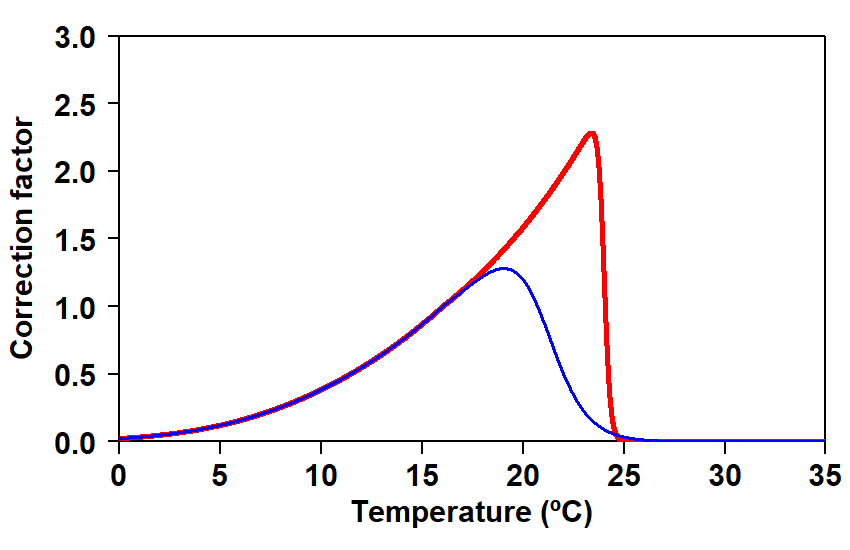
\includegraphics[width=1.0\textwidth]{figures/Chap3CT_curves.png}
	\centering
	\caption{Temperature correction curves for the metabolic flux in the dynamic energy budget model (eqn. \ref{C_T}); blue and red curve correspond respectively to Case 1 and Case 2 in Table 1.}
	\label{Chap3CT_curves}
\end{figure}

\subsection{Ichthyop-DEB model coupling implementation}\label{Chap3Ich-DEBstd}

Jorge Flores-Valiente et al.\\

The following description is a simplification of the \gls{encrasicolus} \acrshort{deb} model developed by \cite{PethRoos2013} as we only focus on the embryo and larva stages. We implemented these equations in the Lagrangian tool routines of \gls{ich} \citep{LettVerl2008} to develop \gls{ich-deb}.\\

\begin{figure}[ht]
	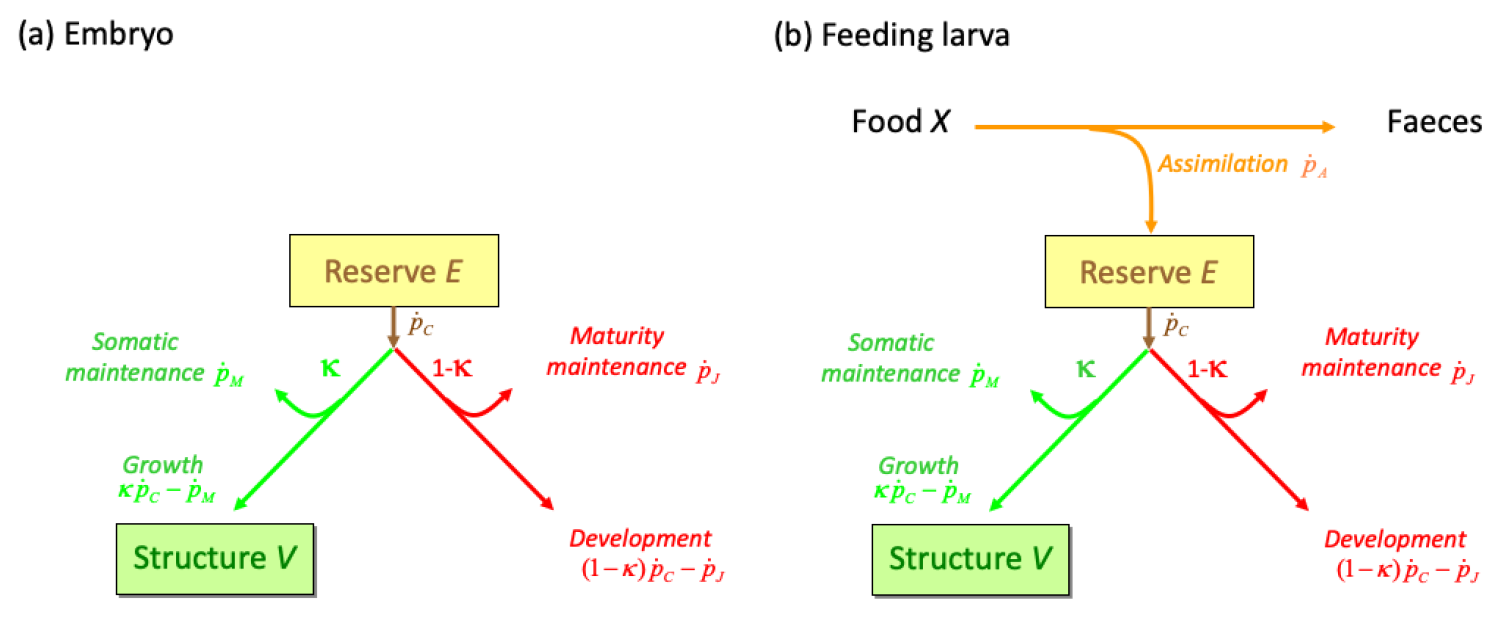
\includegraphics[width=1.0\textwidth]{figures/Chap3DEBflux.png}
	\centering
	\caption{Schemes of the energy fluxes of a \acrlong{deb} model (a) for the embryo stage (non-feeding stage) and (b) the feeding larval stage.}
	\label{Chap3DEBflux}
\end{figure}

\subsubsection{Forcing variables}\label{Chap3ForVar}
\hfill \\

$T$ Temperature ($K$) is the water temperature surrounding an individual (modeled by CROCO-PISCES)\\

$X$ Food density averaged Mesozooplankton field ($\left[ \mu mol CL^{-1} \right]$) over the water column (modeled by CROCO-PISCES)\\

\subsubsection{Initial conditions of state variables (egg stage)}\label{Chap3InitCond}

The age of the individual is set at zero on the day of spawning.\\

\begin{table}
\centering
\rowcolors{1}{white}{gris}
\begin{tabular}{c|c|c|c}
\toprule
Symbol		& 
Value		& 
Units		& 
Definition	\\ 
\midrule
$E$				& 
$0.99$			& 
$J$				& 
Initial Reserve	\\ 
$V$     			& 
$0.000001$			& 
$mm^3$				& 
Initial Structure	\\
\bottomrule
\end{tabular} 
\end{table}

\subsubsection{Primary parameters}\label{Chap3PriPar}

\begin{table}[H]
\centering
\rowcolors{1}{white}{gris}
\begin{adjustbox}{width=1.2\textwidth}
\begin{tabular}{l|l|l|l}
\toprule
\multicolumn{4}{l}{
	Primary parameters (rates are at reference temperature $T_{1} = 293 K$  ($=20$\textdegree $C$)} \\
\midrule
Symbol		& 
Value		& 
Unit		&
Definition	\\
\midrule
$Lw_{h}$		& 
0.28			& 
$cm$			& 
Hatch length	\\
$Lw_{b}$									& 
0.35									& 
$cm$									& 
Yolk-sac to feeding larva threshold		\\
$T_{A}$					& 
9800					& 
$K$						& 
Arrhenius temperature	\\
$T_{L}$						& 
279/279						& 
$K$							& 
Lower temperature boundary	\\
$T_{H}$							& 
294/297							& 
$K$								& 
Upper temperature boundary		\\
$T_{AL}$									& 
20000/20000									& 
$K$											& 
Arrhenius temperature for lower boundary	\\
$T_{AH}$										& 
95000/570000									& 
$K$												& 
Arrhenius temperature for upper boundary		\\
$K$							& 
1.6							& 
$\mu mol CL^{-1}$			& 
Half-saturation constant	\\
$\kappa_{\mathrm{x}}$						& 
0.71										& 
-											& 
Fraction of food energy fixed in reserve	\\
$\left\{\dot{p}_\mathrm{Xm} \right\}$			& 
516												& 
$J.cm^{-2}.d^{-1}$								& 
Maximum surface-specific ingestion rate		\\
$\left[E_{m} \right]$		& 
2700						& 
$J.cm^{-3}$					& 
Maximum reserve density		\\
$\left[E_{G} \right]$				& 
4000								& 
$J.cm^{-3}$							& 
Volume-specific costs of structure	\\
$\left[\dot{p}_{M} \right]$					& 
76.22										& 
$J.cm^{-3}.d^{-1}$							& 
Volume-specific somatic maintenance rate	\\
$\kappa$																	& 
0.7																			& 
-																			& 
Fraction of mobilized reserve allocated to growth and somatic maintenance	\\
\bottomrule
\end{tabular}
\end{adjustbox}
\end{table}

\subsubsection{Auxiliary and compounds parameters}

\begin{table}[H]
\centering
\begin{adjustbox}{width=1.2\textwidth}
\begin{tabular}{l|l|l|l}
\toprule
\multicolumn{4}{l}
	{Auxiliary and Compounds parameters}   \\
\midrule
Symbol		& 
Value		& 
Unit		& 
Definition	\\
\midrule
$\delta_{M}$		& 
0.152				& 
-					& 
Shape coefficient	\\
$\left \{ \dot{p}_\mathrm{Am} \right \}$								& 
$\kappa_{\mathrm{x}} $ $\left \{ \dot{p}_\mathrm{Xm} \right \}=366$	& 
$J.cm^{-2}.d^{-1}$														& 
Maximum surface-area-specific assimilation rate						\\
\bottomrule
\end{tabular}
\end{adjustbox}
\end{table}

\subsubsection{Scaled functional response}\label{Chap3resp_f}
\hfill \\

$V_{b} = (\delta_{M}Lw_{b})^3$ \hfill Structural volume at first-feeding in $cm^3$.\\

\textbf{if} $(V < V_{b})$ \\

$f = 0$ \hfill No feeding.\\

\textbf{else}\\

$f= \frac{X}{X+K}$	    \hfill Feeding.\\

\subsubsection{Temperature correction}\label{Chap3cT_corr}
\hfill \\

Each rate parameter is corrected for temperature according to the following equation \citep{Kooi2009}.\\

$
	C_{T} = exp\left ( \frac{T_{A}}{T_{1}} - \frac{T_{A}}{T} \right )
	\left ( \frac
				{1+exp\left ( \frac{T_{AL}}{T_{1}} - \frac{T_{AL}}{T_{L}} \right )
				  +exp\left ( \frac{T_{AH}}{T_{H}} - \frac{T_{AH}}{T_{1}} \right )}
				{1+exp\left ( \frac{T_{AL}}{T} - \frac{T_{AL}}{T_{L}} \right )
				  +exp\left ( \frac{T_{AH}}{T_{H}} - \frac{T_{AH}}{T} \right )}
	\right )
$\\

With $T_{1}$ the reference temperature (at which flux parameters were estimated), $T_{A}$ is the Arrhenius temperature and $T_{AH}$, $T_{AH}$, $T_{L}$, $T_{H}$ are constants used to define a curved shape of the temperature correction according to temperature.\\

$\left \{ \dot{p}_\mathrm{Am} \right \}_{T} = C_{T} \left \{ \dot{p}_\mathrm{Am} \right \}_{T_{1}}$\\

$\left [ \dot{p}_{M} \right ]_{T} = C_{T} \left [ \dot{p}_{M} \right ]_{T_{1}}$\\

\subsubsection{Fluxes ($Jd^{-1}$)}\label{Chap3Fluxex}
\hfill \\

$\dot{p}_\mathrm{A} = f \left \{ \dot{p}_\mathrm{Am} \right \}_{T} V^{2/3}$ \hfill Assimilation.\\

$\dot{p}_\mathrm{M} = \left [ \dot{p}_{M} \right ]_{T} V$ \hfill Volume-related somatic maintenance.\\


	$\dot{p}_{C} = \frac
					   {E\left ( \left [ E_{G} \right ] \frac{C_{T}\left \{ \dot{p}_\mathrm{Am} \right \}_{T}}{\left [ E_{m} \right ]} V^{-\frac{1}{3}}+\left [ \dot{p}_{M} \right ]_{T}\right )}
					   {\kappa\left ( \frac{E}{V} \right ) + \left [ E_{G} \right ]}$ \hfill Mobilization of energy.\\

$\dot{p}_{G} = \kappa \dot{p}_{C} - \dot{p}_\mathrm{M}$ \hfill Energy directed to structural growth.\\

$\dot{p}_{J} = V \frac{\left ( 1 - \kappa \right )}{\kappa}\left [ \dot{p}_{M} \right ]_{T}$ \hfill Maturity maintenance (for $V < V_{p}$ (Structural volume at puberty), the condition is always TRUE because in \gls{ich-deb} the complexity level of the organism at puberty is never exceeded, as we only consider embryos and larvae).\\

Starvation test\\

\textbf{if} $\kappa \dot{p}_{C} < \dot{p}_\mathrm{M}$ or $\left ( 1- \kappa \right ) \dot{p}_{C} < \dot{p}_{J}$\\

$starvation = 1$ \hfill Individual (or super-individual) removed from population.\\

\textbf{else}\\

$starvation = 0$ \hfill Individual continues in the simulation.\\

\subsubsection{Differential equations}\label{Chap3DiffEq}
\hfill \\

$\frac{dE}{dt} = \dot{p}_\mathrm{A} - \dot{p}_{C}$ \hfill Reserve dynamics.\\

$\frac{dV}{dt} = \frac{\dot{p}_{G}}{\left[ E_{G} \right]}$ \hfill Structure dynamics.\\

\subsubsection{Integration}\label{Chap3Integ}
\hfill \\
$E\left ( t + \Delta t \right ) = E\left ( t \right ) + \frac{dE}{dt}\Delta t$ \\

$V\left ( t + \Delta t \right ) = V\left ( t \right ) + \frac{dV}{dt}\Delta t$ \\

With $\Delta t = 0.083 d \left (=2hours\right )$

\subsubsection{Observable variables}\label{Chap3ObsVar}
\hfill \\
$L_{w} = \frac{V^{1/3}}{\delta_{M}}$ \hfill Physical length ($cm$).\\

where $L_{w}$ is the standard length $SL$ ($cm$), $V$ the structural volume ($cm^3$) and $\delta_{M}$ a shape coefficient.\\

We assume that the larva does not change in shape till it reaches our length criteria of $2cm$ (SL) and that there is a constant proportionality ($\delta_{M}$) between structural volume and length.\\


\clearpage
\section{Results of climatological simulations}\label{Chap3Resu1}

In general, the bioenergetic model of European anchovy (\textit{\gls{encrasicolus}}), developed by \cite{PethRoos2013}, simulated well the larval growth patterns of \textit{\gls{ringens}} for different temperatures and compared with individuals reared in the laboratory (15, 18, 19 \textdegree C, \cite{RiouOfel2021}) and individuals sampled from the natural environment (16ºC, \cite{MoreClar2011}). The average simulated growth (colored solid lines) demonstrates an acceptable fit to laboratory and literature data, as shown in Fig. \ref{Chap3DEBvsData}.

\begin{figure}[H]
	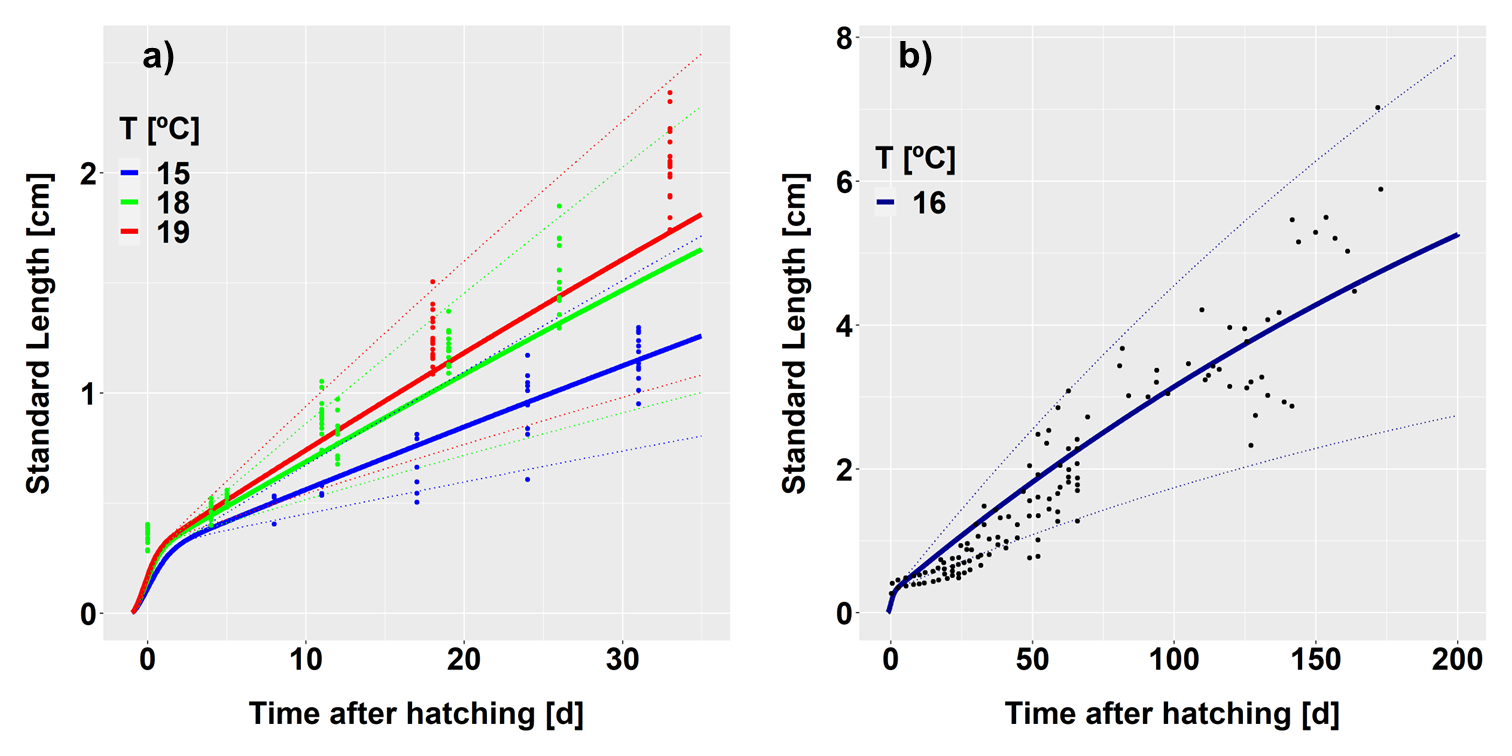
\includegraphics[width=1.0\textwidth]{figures/Chap3DEBvsData.png}
	\centering
	\caption{Comparison of Peruvian anchovy simulated larval growth and laboratory
observations from \cite{RiouOfel2021} (a) and in situ observations from \cite{MoreClar2011}
(b). Thick lines correspond to average size predictions considering ten $f$ values from 0.1 to 1
with 0.1 steps (food limitation factor, see section \ref{Chap3Ich-DEBstd}) at 19°C (red), 18°C (green) and 15°C (blue) in (a) and at 16°C in (b). Dotted lines correspond to standard deviation of the simulated larval growth. Colored dots show the corresponding observations. The bioenergetic model
parameters were taken from \cite{PethRoos2013}. Note that the scales are different in the
two panels.}
	\label{Chap3DEBvsData}
\end{figure}

Globally, in $Sim 4$ we obtained similar retention patterns as \cite{BrocLett2008}, who used different physical forcing fields. The interaction of spawning depth and month displayed the same characteristic pattern, with highest retention in austral winter for the superficial spawning depth level (0 - 15 $m$) and in summer for the deepest spawning levels (30 - 45 $m$; bars in Fig. \ref{Chap3BrocVSFloreBarplots}). We also found the same seasonal trends when the spawning area was split into inner shelf (0 - 100 $m$ isobaths) and offshore shelf (100 - 500 $m$ and 500 - 2000 $m$ isobaths; lines in Fig. \ref{Chap3BrocVSFloreBarplots}). The results differed most in the zone between 14\textdegree S to 16\textdegree S with highest values obtained from July to October in \cite{BrocLett2008}, as opposed to a maximum in January-February obtained here (Fig. \ref{Chap3BrocVSFloreHovmuller}).\\

\begin{figure}[H]
	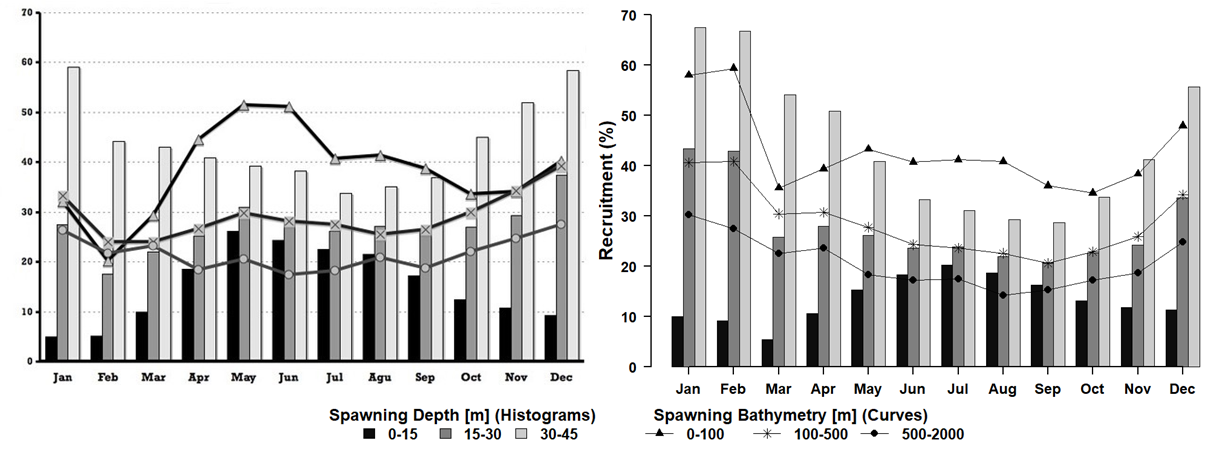
\includegraphics[width=1.0\textwidth]{figures/Chap3BrocVSFloreBarplots.png}
	\centering
	\caption{Percentage of recruited larvae of Peruvian anchovy obtained for different spawning months, spawning depths, and isobaths delimiting spawning areas horizontally from \cite{BrocLett2008} (left) and from $Sim 4$ (right).}
	\label{Chap3BrocVSFloreBarplots}
\end{figure}

\begin{figure}[H]
	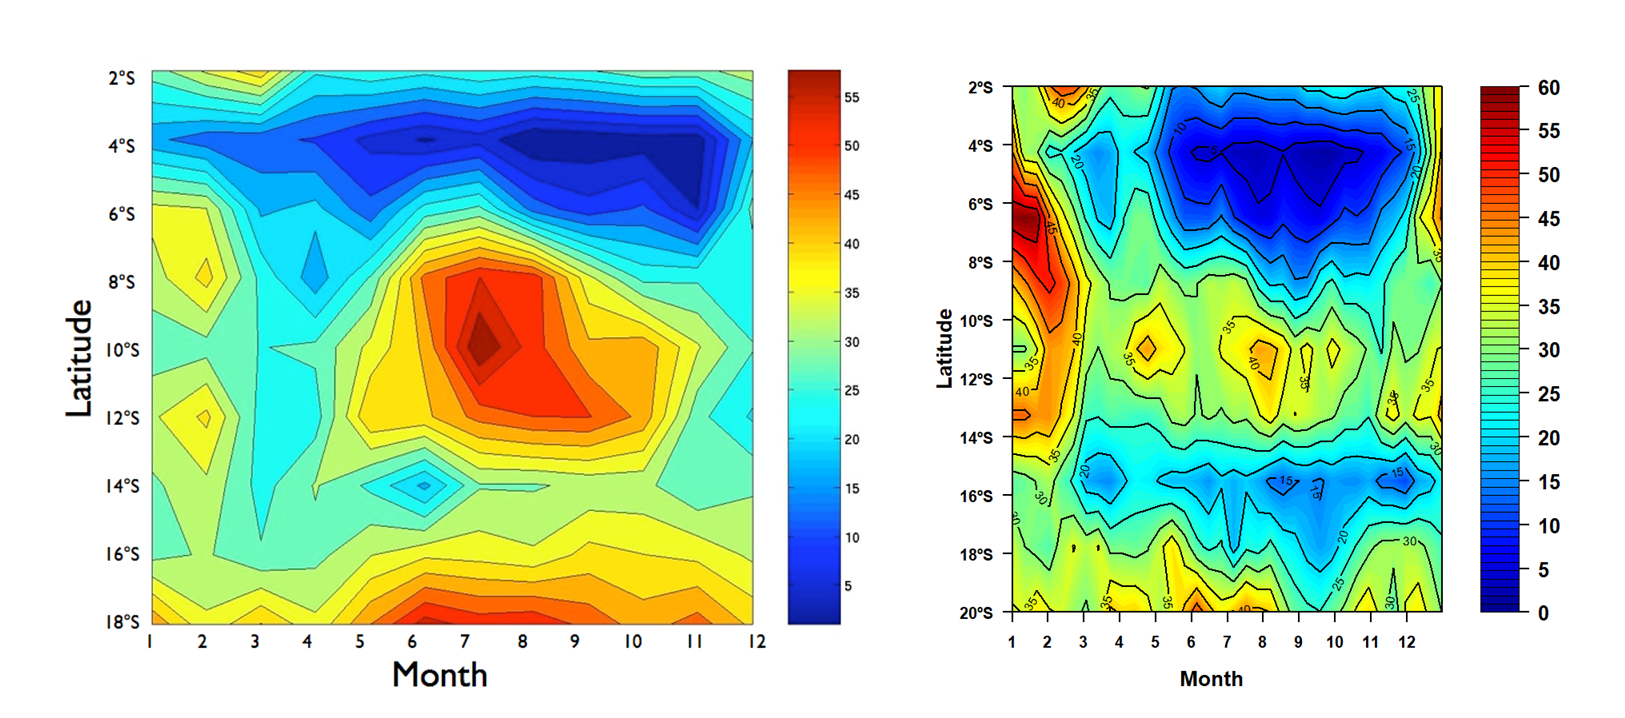
\includegraphics[width=1.0\textwidth]{figures/Chap3BrocVSFloreHovmuller.png}
	\centering
	\caption{Percentage of recruited larvae of Peruvian anchovy obtained for different months and latitudes from (left) \cite{BrocLett2008} and (right) $Sim 4$.}
	\label{Chap3BrocVSFloreHovmuller}
\end{figure}

The analysis of variance (ANOVA, Table \ref{Chap3ANOVAsim5}) applied to recruitment rates for Case 1 ($Sim 5$) indicates that spawning depth had the greatest effect on recruitment rates (28.35 \%), followed by latitude (14.26 \%). The other factors (spawning bathymetry, spawning month, and spawning year) showed less than 3 \% of the variance in recruitment rates. However, the combined effect of spawning month and spawning latitude explained 11.26 \% of the variance, followed by spawning month combined with spawning depth (9.20 \%). The remaining combinations did not exceed 4 \% percent explanation.\\

%\begin{landscape}
\begin{table}[H]
\centering
\caption{ANOVA of recruitment rates for $Sim 5$ (Case 1).}
\rowcolors{1}{white}{gris}
\begin{adjustbox}{width=0.9\textwidth}
\small
\begin{tabular}{c|r|r|r|r|r|r}
\toprule
                                  &
	\textbf{Df}                   &
	\textbf{Sum Sq}               &
	\textbf{Mean Sq}              &
	\textbf{F-value}    		   &
	\textbf{Pr (\textgreater{F})} &
	$\mathbf{\% Exp}$      \\
\midrule
Year                  & 2    & 594.61    & 297.31    & 3.71    & 0.02                & 0.02  \\
Month                 & 11   & 46972.03  & 4270.18   & 53.28   & 0.00                & 1.82  \\
Depth                 & 2    & 729892.48 & 364946.24 & 4553.68 & 0.00                & 28.35 \\
Bathymetry            & 2    & 77575.46  & 38787.73  & 483.98  & 0.00                & 3.01  \\
Latitude              & 8    & 367107.93 & 45888.49  & 572.58  & 0.00                & 14.26 \\
Year x Month          & 22   & 13008.37  & 591.29    & 7.38    & 0.00                & 0.51  \\
Year x Depth          & 4    & 355.96    & 88.99     & 1.11    & 0.35                & 0.01  \\
Year x Bathymetry     & 4    & 607.77    & 151.94    & 1.90    & 0.11                & 0.02  \\
Year x Latitude       & 16   & 9125.50   & 570.34    & 7.12    & 0.00                & 0.35  \\
Month x Depth         & 22   & 236883.93 & 10767.45  & 134.35  & 0.00                & 9.20  \\
Month x Bathymetry    & 22   & 32948.88  & 1497.68   & 18.69   & 0.00                & 1.28  \\
Month x Latitude      & 88   & 290053.41 & 3296.06   & 41.13   & 0.00                & 11.26 \\
Depth x Bathymetry    & 4    & 3913.28   & 978.32    & 12.21   & 0.00                & 0.15  \\
Depth x Latitude      & 16   & 78663.56  & 4916.47   & 61.35   & 0.00                & 3.06  \\
Bathymetry x Latitude & 12   & 108870.81 & 9072.57   & 113.20  & 0.00                & 4.23  \\
Residuals             & 7216 & 578313.56 & 80.14     &         &                     & 22.46 \\
\bottomrule
\end{tabular}
\end{adjustbox}
\label{Chap3ANOVAsim5}
\end{table}
%\end{landscape}

In Case 2 ($Sim 6$), the results of the ANOVA (Table \ref{Chap3ANOVAsim6}) indicated that spawning depth had the greatest effect on recruitment rates (20.71 \%), followed by latitude (13.19 \%) and month of spawning (9.48 \%). The remaining factors (spawning bathymetry and spawning year) collectively accounted for less than 5 \% of the variance. The combined effect of spawning month and latitude explained 8.77 \% of the variance, while the combined effect of spawning month and depth explained a value similar to the previous one (8.04 \%). Another noteworthy combination was that of bathymetry and spawning latitude (6.58 \%). The remaining combinations did not demonstrate particularly noteworthy values.\\

When we included larval growth ($Sim 5$ and $Sim 6$) and changed the criterion used for retention from age ($Sim 4$, 30 days, grey bars) to size ($Sim 5$ and $Sim 6$; $>$ 2 $cm$, black line) we obtained nearly identical results, except when mortality ($Sim 5$ and $Sim 6$; red line) was further included then small differences occurred in simulated recruitment patterns (Fig. \ref{Chap3Case1CriterionCompar} and Fig. \ref{Chap3Case2CriterionCompar}, respectively). In Case 1 ($Sim 5$), when the bio-energetic fluxes decayed smoothly at high temperature, the seasonal pattern remained similar using recruitment criteria 1,2 and 3 favoring summer months (Fig. \ref{Chap3Case1CriterionCompar}a). Latitudinal range between 6\textdegree - 14\textdegree S showed the highest recruitment value using recruitment criteria 1,2 but using criterion 3 only the zone between 6\textdegree - 8\textdegree $S$ was the most important (Fig. \ref{Chap3Case1CriterionCompar}b).\\

%\begin{landscape}
\begin{table}[H]
\centering
\caption{ANOVA of recruitment rates for $Sim 6$ (Case 2).}
\rowcolors{1}{white}{gris}
\begin{adjustbox}{width=0.9\textwidth}
\small
\begin{tabular}{c|r|r|r|r|r|r}
\toprule
                                  &
	\textbf{Df}                   &
	\textbf{Sum Sq}               &
	\textbf{Mean Sq}              &
	\textbf{F-value}    		   &
	\textbf{Pr (\textgreater{F})} &
	$\mathbf{\% Exp}$      \\
\midrule
Year                  & 2    & 645.96    & 322.98    & 3.09    & 0.05                & 0.02  \\
Month                 & 11   & 322491.73 & 29317.43  & 280.91  & 0.00                & 9.48  \\
Depth                 & 2    & 704668.20 & 352334.10 & 3375.96 & 0.00                & 20.71 \\
Bathymetry            & 2    & 163298.92 & 81649.46  & 782.34  & 0.00                & 4.80  \\
Latitude              & 8    & 448898.07 & 56112.26  & 537.65  & 0.00                & 13.19 \\
Year x Month          & 22   & 12459.78  & 566.35    & 5.43    & 0.00                & 0.37  \\
Year x Depth          & 4    & 744.83    & 186.21    & 1.78    & 0.13                & 0.02  \\
Year x Bathymetry     & 4    & 578.29    & 144.57    & 1.39    & 0.24                & 0.02  \\
Year x Latitude       & 16   & 10171.15  & 635.70    & 6.09    & 0.00                & 0.30  \\
Month x Depth         & 22   & 273637.25 & 12438.06  & 119.18  & 0.00                & 8.04  \\
Month x Bathymetry    & 22   & 31626.91  & 1437.59   & 13.77   & 0.00                & 0.93  \\
Month x Latitude      & 88   & 298338.78 & 3390.21   & 32.48   & 0.00                & 8.77  \\
Depth x Bathymetry    & 4    & 4990.27   & 1247.57   & 11.95   & 0.00                & 0.15  \\
Depth x Latitude      & 16   & 153670.06 & 9604.38   & 92.03   & 0.00                & 4.52  \\
Bathymetry x Latitude & 12   & 223998.82 & 18666.57  & 178.86  & 0.00                & 6.58  \\
Residuals             & 7216 & 753101.16 & 104.37    &         &                     & 22.13 \\
\bottomrule
\end{tabular}
\end{adjustbox}
\label{Chap3ANOVAsim6}
\end{table}
%\end{landscape}

The same typical direct relationship was observed between spawning depth and larval retention for criterion 1,2 and 3 (Fig. \ref{Chap3Case1CriterionCompar}c) and recruitment values were higher when spawning was close to the coast (0 - 100 $m$) for all 3 criteria (Fig. \ref{Chap3Case1CriterionCompar}d). In Case 2 ($Sim 6$), when mortality was included (criterion 3), we obtained a stronger seasonal variability highlighting the difference between summer and winter (Fig. \ref{Chap3Case2CriterionCompar}a) and highest values for the northern part of the domain (2\textdegree - 4\textdegree S) instead of the central zone without mortality (Fig. \ref{Chap3Case2CriterionCompar}b). Most notably, recruitment was highest for the intermediate spawning depth level (15 - 30 $m$) as opposed to highest for the deepest depth level (30 - 45 $m$) without mortality (Fig. \ref{Chap3Case2CriterionCompar}c). Including mortality, the importance of the near-shore area (0 - 100 $m$) was emphasized (Fig. \ref{Chap3Case2CriterionCompar}d).\\

A food limitation sensitivity test between $Sim 7$ (Case 1, food limitation) and $Sim 5$ (Case 1, no food limitation) showed that food acted as a growth limiting factor. Food was observed to be a significant constraint to recruitment during the winter months (black line), further highlighted when a mortality rate was applied (red dotted line) (Fig. \ref{Chap3Case1f1}a). Spatially, this limitation was concentrated in the area between 14\textdegree - 16\textdegree $S$ (black line), and although a constant mortality rate was applied, this pattern remained similar (red dashed line, Fig. \ref{Chap3Case1f1}b). When individuals were spawned at a shallower depth, a slightly greater limitation was observed compared to deeper zones, although less evident than those previously mentioned (black and dotted red line, Fig. \ref{Chap3Case1f1}c). Finally, no clear pattern of food limitation related to spawning bathymetry was observed (Fig. \ref{Chap3Case1f1}d). In Case 2, the same seasonal (Fig. \ref{Chap3Case2f1}a) and spatial (Fig. \ref{Chap3Case2f1}b) pattern of food limitation is observed. However, when a mortality rate is applied (red dotted line, Fig. \ref{Chap3Case2f1}c,d), slight limitations in spawning depth and bathymetry become evident.\\

At the surface layer (0 - 15 $m$), winter spawning months favored \textit{\gls{ringens}} recruitment when using an age-criterion (Fig. \ref{Chap3DepthLevels}a) and a size-criterion in Case 1 (Fig. \ref{Chap3DepthLevels}d) whereas in Case 2 (Fig. \ref{Chap3DepthLevels}g) recruitment tended to be uniform over months. By contrast, in intermediate layers (15 - 30 $m$) summer months for spawning favored recruitment when using an age-criterion (Fig. \ref{Chap3DepthLevels}b) and a size-criterion in Case 2 (Fig. \ref{Chap3DepthLevels}h), whereas in Case 1 (Fig. \ref{Chap3DepthLevels}e) recruitment tended to become uniform. In deeper layers (30 - 45 $m$), summer favored recruitment in all cases (Fig. \ref{Chap3DepthLevels}c, f, i).\\

When mortality was included, Case 1 at the surface layer (0 - 15 $m$, Fig. \ref{Chap3DepthLevelsMortality}d) lead to fairly low and uniform recruitment whereas all other cases showed highest recruitment in summer (Fig. \ref{Chap3DepthLevelsMortality}a, b, c, e, f, g, h, i).\\

\begin{figure}[H]
	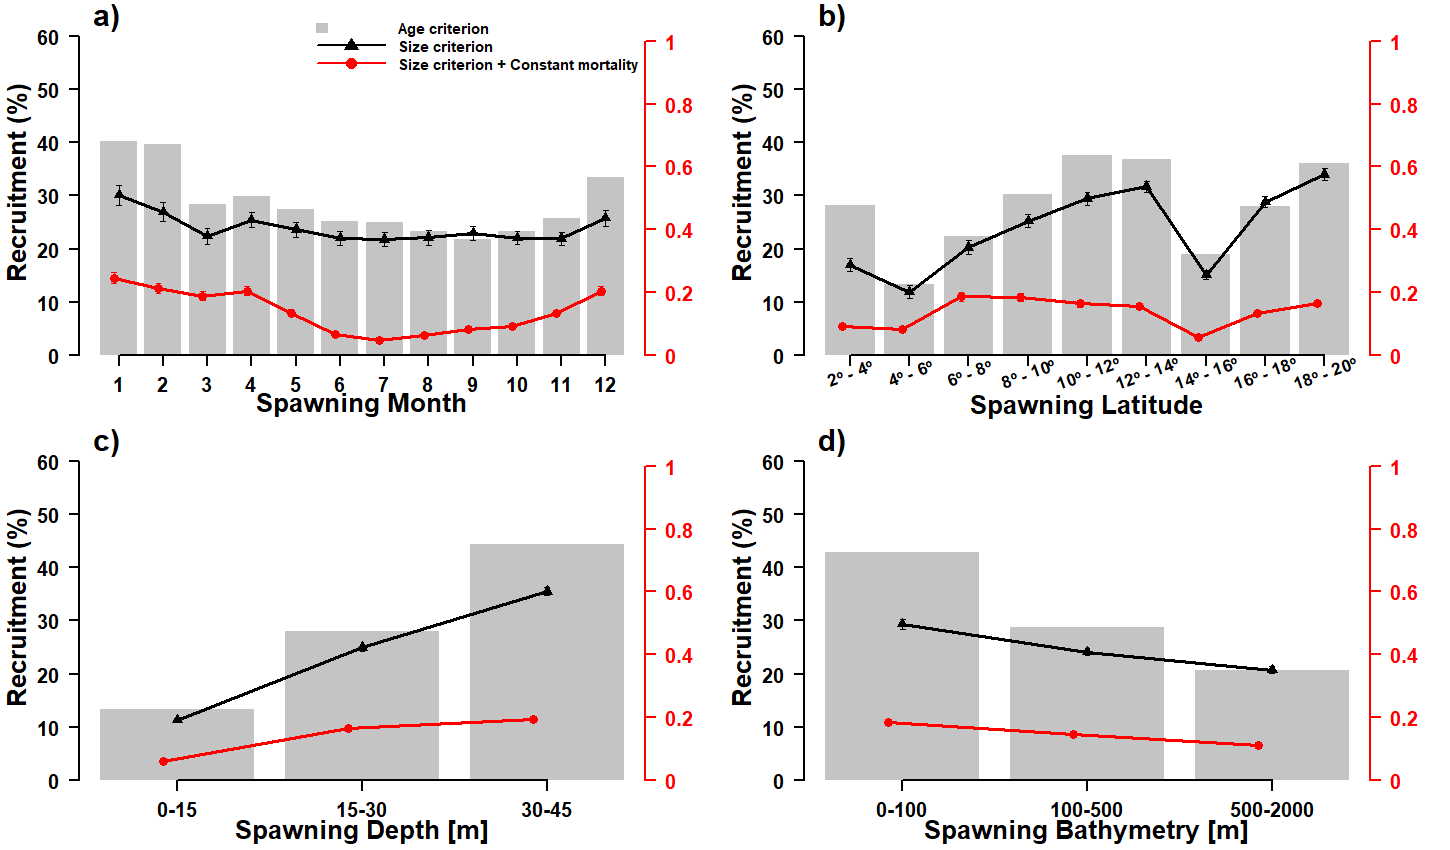
\includegraphics[width=1.0\textwidth]{figures/Chap3Case1CriterionCompar.png}
	\centering
	\caption{Percentage of recruited larvae of Peruvian anchovy obtained for different a) spawning months, b) spawning latitudes, c) spawning depths and d) isobaths delimiting spawning areas horizontally using different criteria for recruitment (size criteria -black lines-, size criteria plus constant daily mortality -red lines-) in $Sim 5$. Recruitment values based on age criteria -grey bars- were taken from $Sim 4$.}
	\label{Chap3Case1CriterionCompar}
\end{figure}

\begin{figure}[H]
	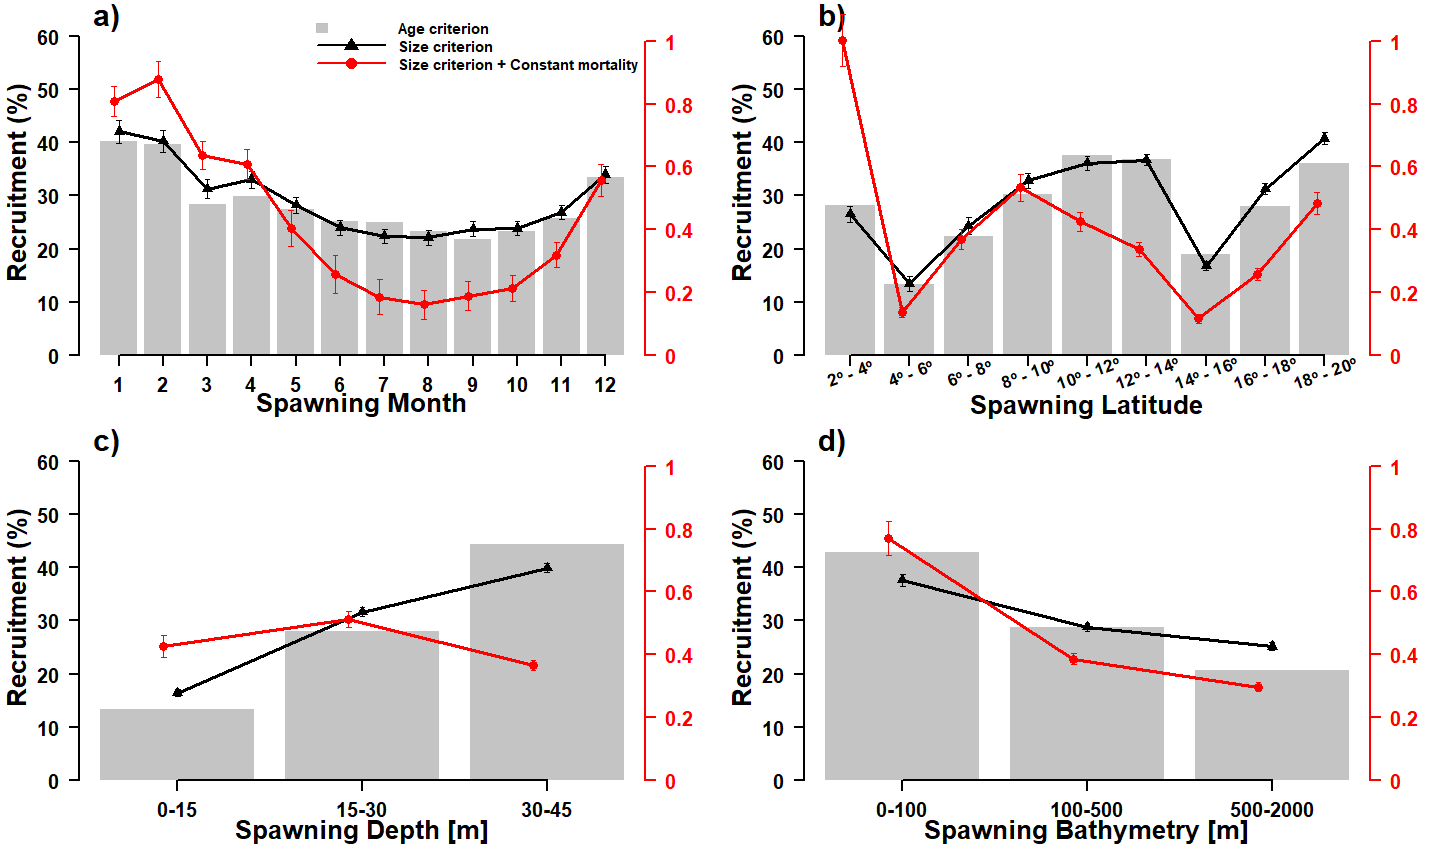
\includegraphics[width=1.0\textwidth]{figures/Chap3Case2CriterionCompar.png}
	\centering
	\caption{Same as Fig. \ref{Chap3Case1CriterionCompar} in $Sim 6$.}
	\label{Chap3Case2CriterionCompar}
\end{figure}

\begin{figure}[H]
	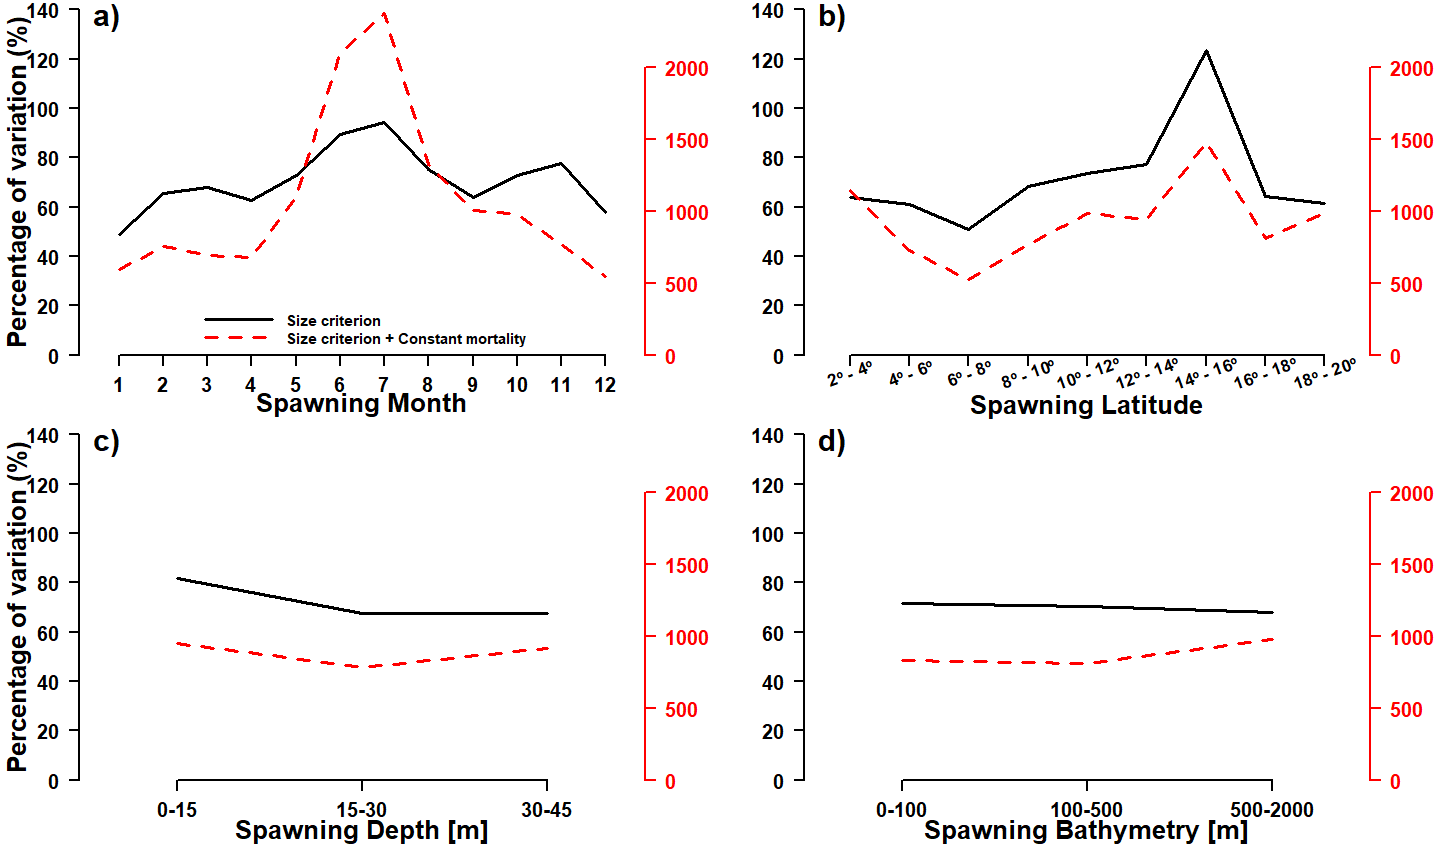
\includegraphics[width=1.0\textwidth]{figures/Chap3Case1f1.png}
	\centering
	\caption{Percentage of variation in recruitment obtained using the size criterion (black line) and the size criterion with mortality included (red dotted line) for $Sim 7$ (Case 1) relatively to $Sim 5$ (Case 1) according to a) spawning month, b) spawning latitude, c) spawning depth and d) spawning bathymetry.}
	\label{Chap3Case1f1}
\end{figure}

\begin{figure}[H]
	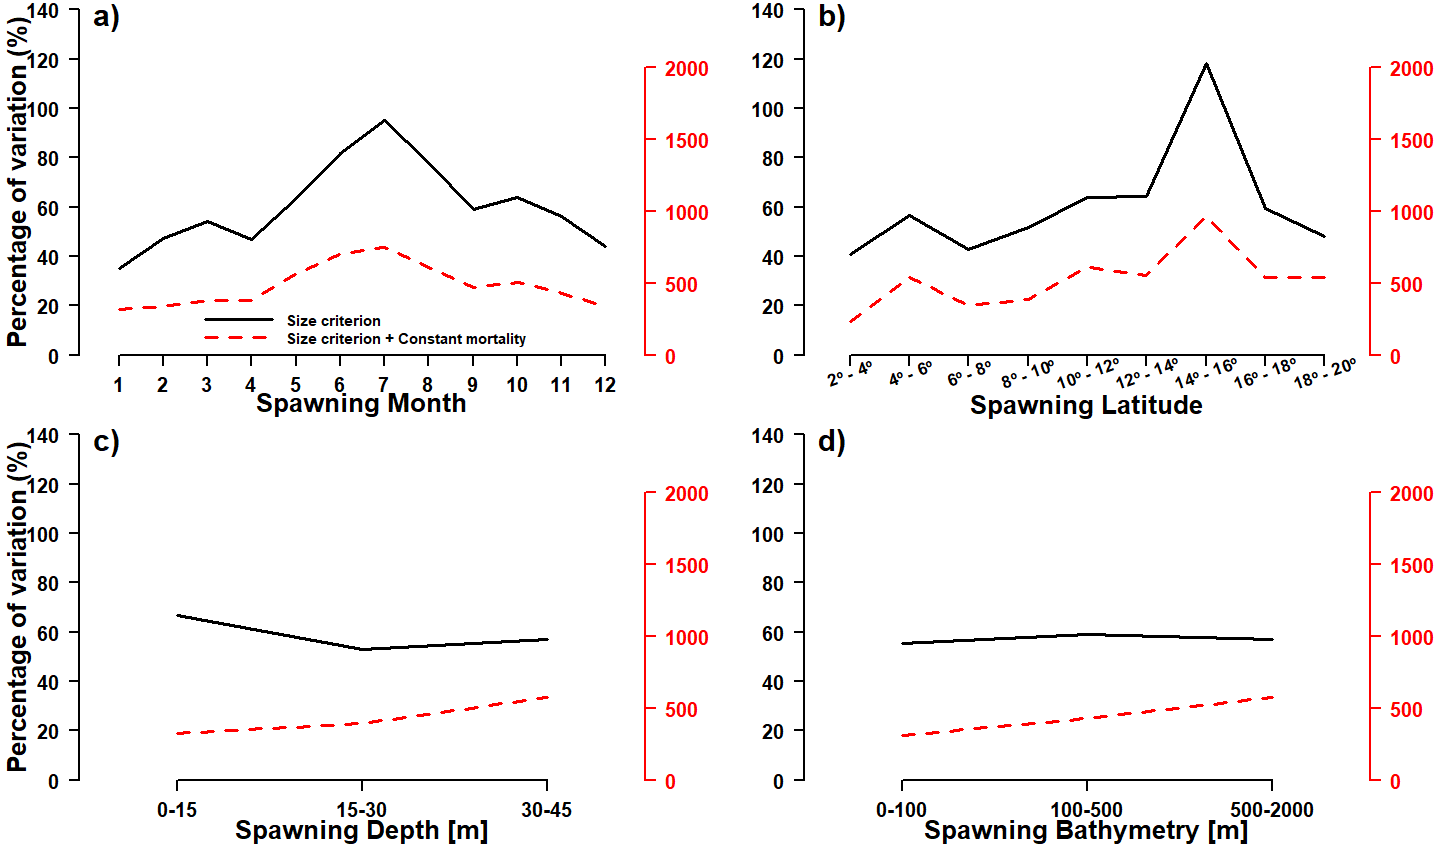
\includegraphics[width=1.0\textwidth]{figures/Chap3Case2f1.png}
	\centering
	\caption{Same as Fig \ref{Chap3Case1f1} but for $Sim 8$ (Case 2) relatively to $Sim 6$ (Case 2}
	\label{Chap3Case2f1}
\end{figure}

\begin{figure}[H]
	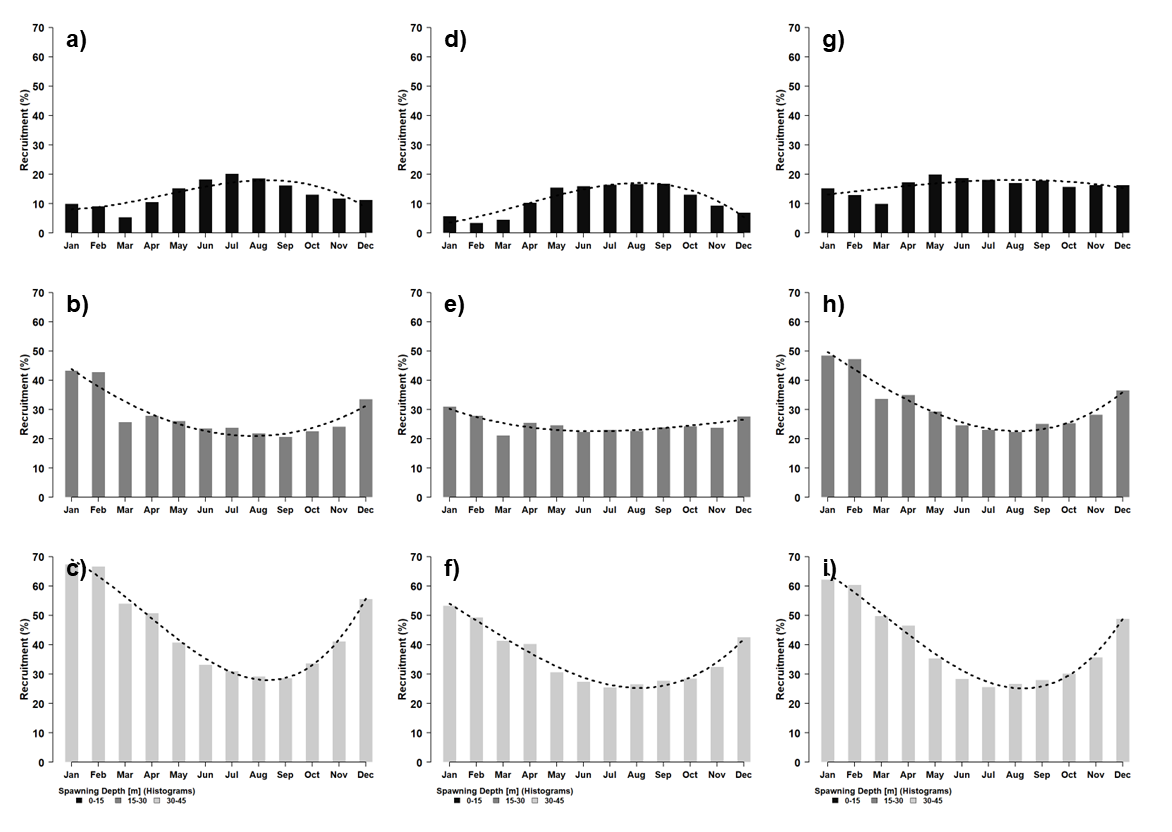
\includegraphics[width=1.0\textwidth]{figures/Chap3DepthLevels.png}
	\centering
	\caption{Percentage of recruited larvae of Peruvian anchovy obtained for different spawning depths in $Sim 4$ criterion 1 (a, b, c), $Sim 5$ criterion 2 (d, e, f) and $Sim 6$ criterion 2 (g, h, i). Spawning depth is (a, d, g) 0 - 15 $m$, (b, e, h) 15 - 30 $m$, (c, f, i) 30 - 45 $m$. The dotted curves are third degree polynomial models fitted to the recruitment patterns.}
	\label{Chap3DepthLevels}
\end{figure}

When a size criterion was used for recruitment (criterion 2), the corresponding age at which individuals recruited was very variable, ranging from 20 to 90 days (Fig. \ref{Chap3MapAgeRecruSim5Sim6}). In $Sim 5$ (Case 1), the central coastal zone of the \acrshort{nhcs} was the most favorable to early recruitment (Fig. \ref{Chap3MapAgeRecruSim5Sim6}a), while $Sim 6$ (Case 2) also favored the central coastal zone and also the northern zone showing much lower recruitment ages than $Sim 5$ (Fig. \ref{Chap3MapAgeRecruSim5Sim6}b). In Case 1, daily recruitment started at an age of $\sim$35 days for all spawning depth levels, and peaked at a similar age of $\sim$50 days (Fig. \ref{Chap3LinesAgeRecruSim5Sim6}a). Upon application of a mortality rate, as illustrated in Fig. \ref{Chap3LinesAgeRecruSim5Sim6}c, recruitment patterns become more uniform. However, a notable change is observed, in which the average depth (15-30 $m$) is slightly more favorable in terms of the age at which individuals are recruited. In Case 2, individuals in the northern part of the \acrshort{nhcs} recruited as early as $\sim$20 days and the daily recruitment peaked at ages $\sim$25, $\sim$35 and $\sim$45 days for depth levels 0 - 15, 15 - 30 and 30 - 45 $m$, respectively (Fig. \ref{Chap3LinesAgeRecruSim5Sim6}b), however, upon application of a mortality rate, it becomes evident that the shallowest zone (0 - 15 $m$) exhibits the greatest degree of favorable recruitment potential (Fig. \ref{Chap3LinesAgeRecruSim5Sim6}d).\\

\begin{figure}[H]
	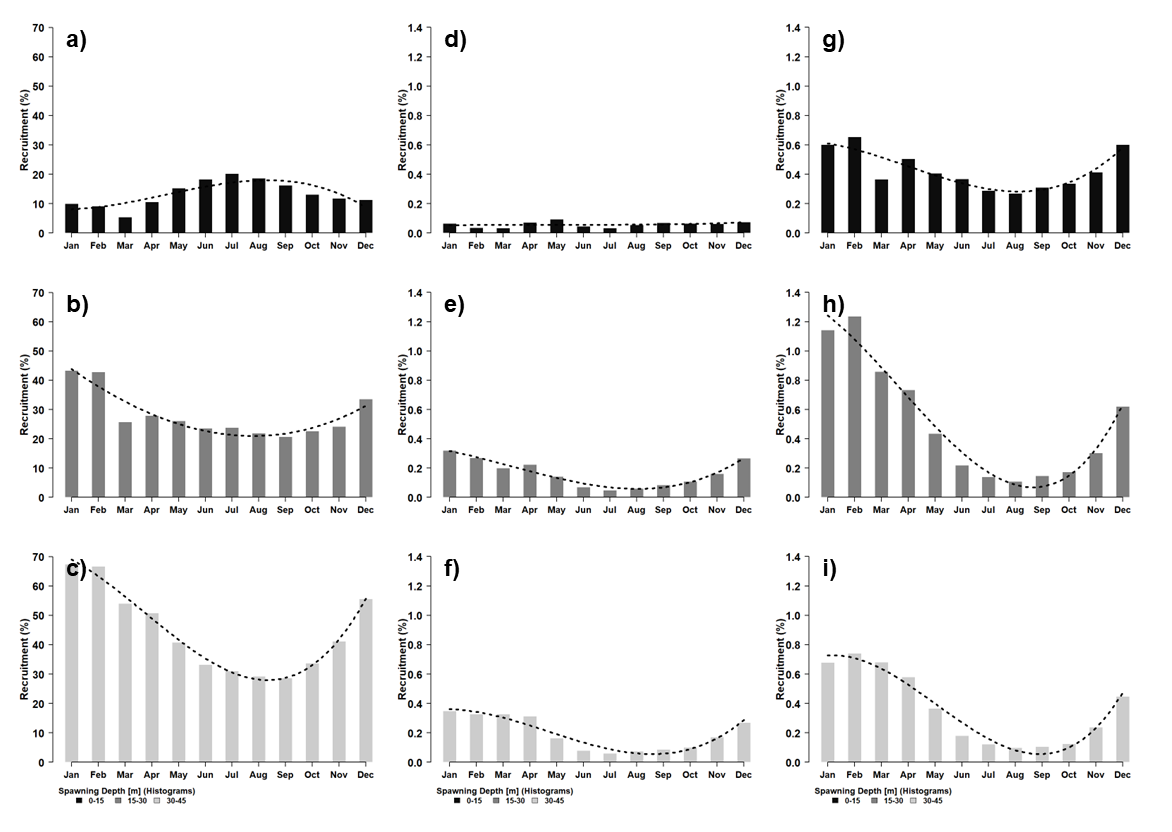
\includegraphics[width=1.0\textwidth]{figures/Chap3DepthLevelsMortality.png}
	\centering
	\caption{Same as Fig. \ref{Chap3DepthLevels} but with mortality included in $Sim 5$ and $Sim 6$ (criterion 3).}
	\label{Chap3DepthLevelsMortality}
\end{figure}

\begin{figure}[H]
	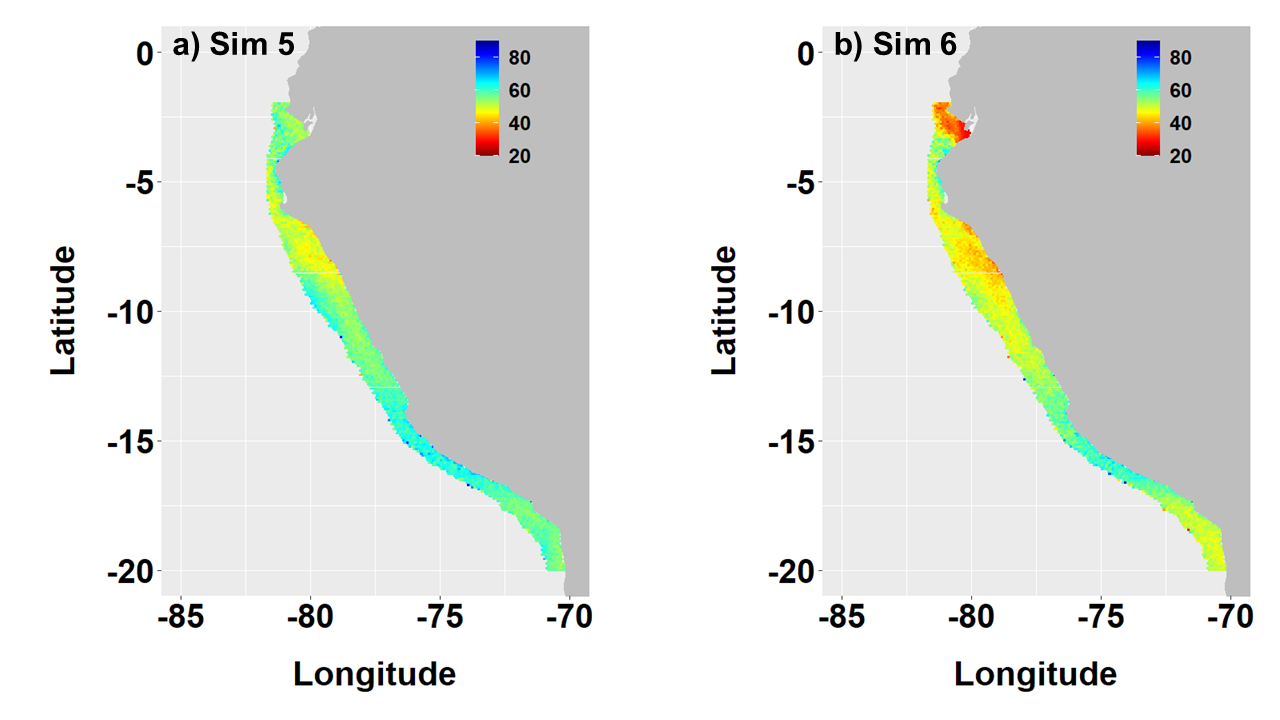
\includegraphics[width=1.0\textwidth]{figures/Chap3MapAgeRecruSim5Sim6.png}
	\centering
	\caption{Spatial distribution of average age at recruitment for a) $Sim5$ and b) $Sim6$.}
	\label{Chap3MapAgeRecruSim5Sim6}
\end{figure}

\begin{figure}[H]
	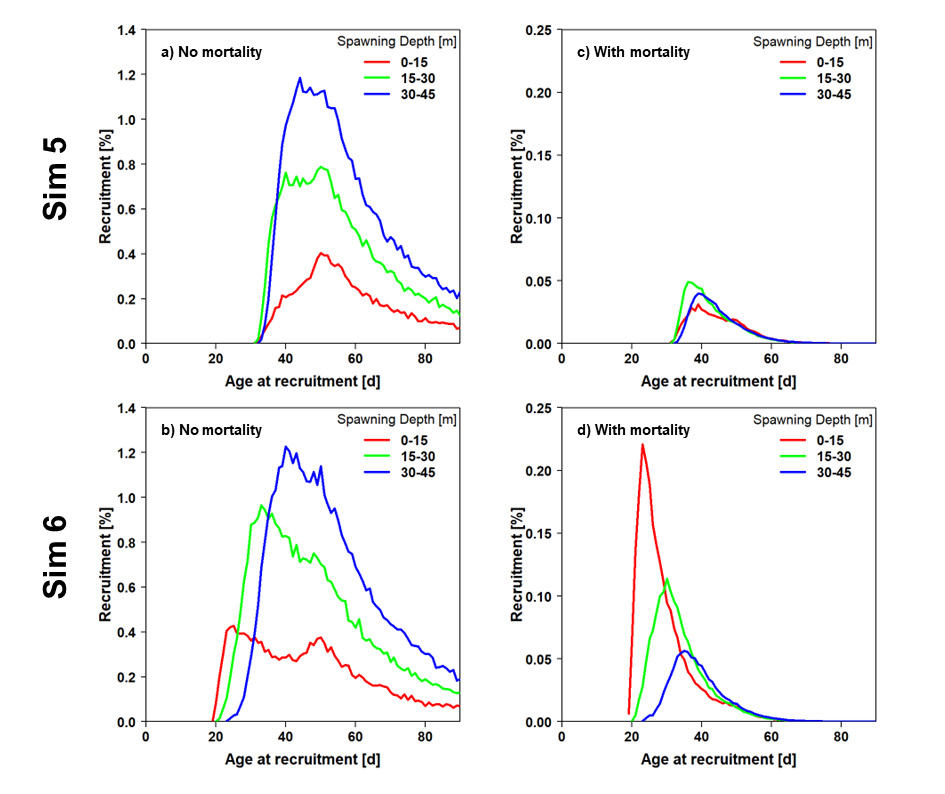
\includegraphics[width=1.0\textwidth]{figures/Chap3LinesAgeRecruSim5Sim6.png}
	\centering
	\caption{Spatial distribution of average age at recruitment for a) $Sim5$ and b) $Sim6$.}
	\label{Chap3LinesAgeRecruSim5Sim6}
\end{figure}

The amount of larvae recruiting according to their spawning location was also very variable along the coast, ranging from 0 to 150 $ind/m^2$ without mortality (Fig. \ref{Chap3DistPartiMapEgg}a, c) and from 0 to 2 $ind/m^2$ cell with mortality (Fig. \ref{Chap3DistPartiMapEgg}c, d). For Case 2 there were three spawning spots favorable to recruitment in the north, center and south of the domain (Fig. \ref{Chap3DistPartiMapEgg}c, d). For Case 1 the northern zone was no longer favorable but the central and southern zones remained (Fig. \ref{Chap3DistPartiMapEgg}a, b), which is more consistent with the spatial distribution of Peruvian anchovy egg density ($eggs/m^2$) derived from field surveys (Fig. \ref{Chap3DistPartiMapEgg}e).\\

\begin{figure}[t]
	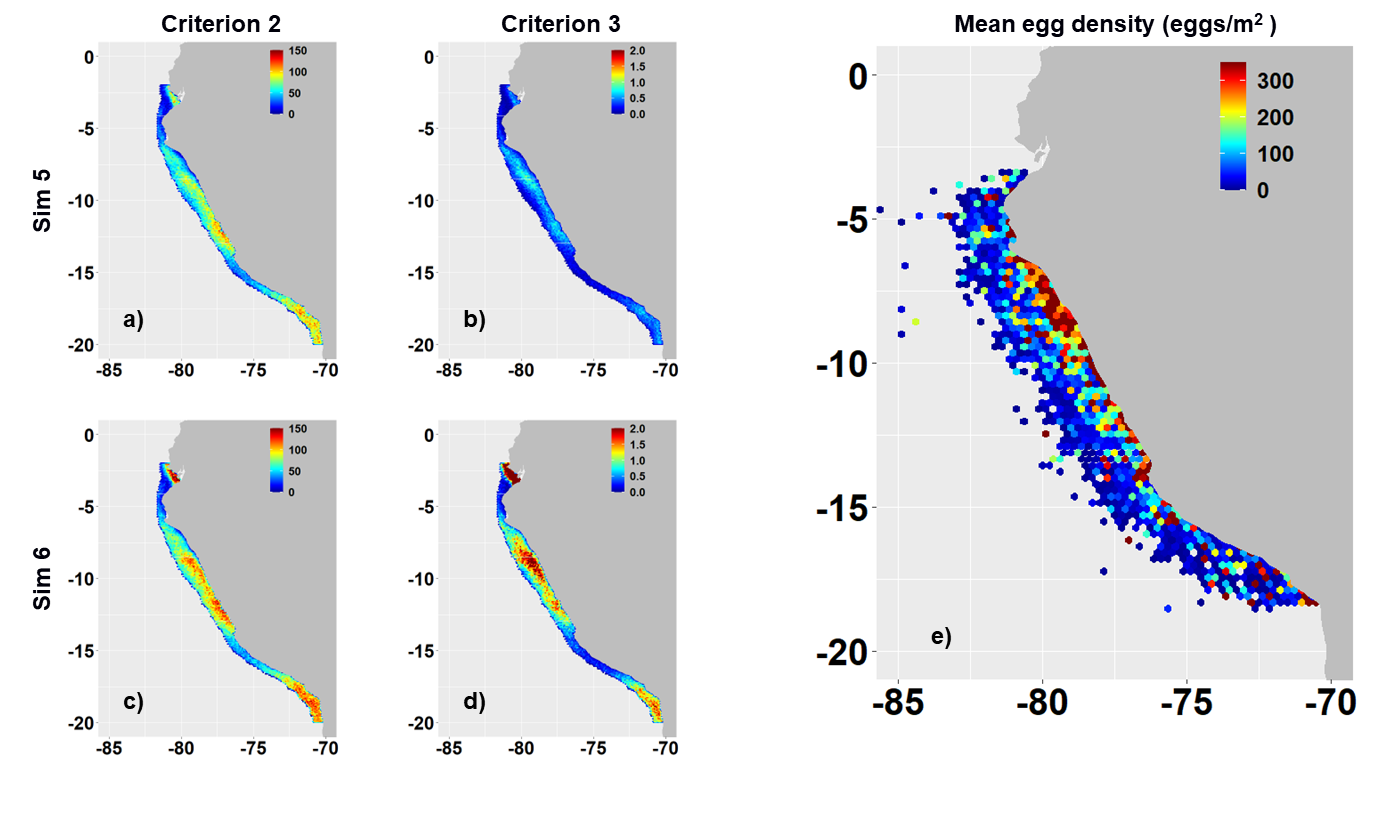
\includegraphics[width=1.0\textwidth]{figures/Chap3DistPartiMapEgg.png}
	\centering
	\caption{Spatial distribution of the average number ($ind/m^2$) of simulated Peruvian anchovy larvae recruiting according to their spawning location obtained with (a, b) $Sim 5$ and (c, d) $Sim 6$ using recruitment criterion 2 (no mortality) (a, c) and 3 (with mortality) (b, d). (e) Spatial distribution of Peruvian anchovy mean egg density ($eggs/m^2$) derived from IMARPE field surveys from year 1961 to 2016. Note that cell grid was 0.1\textdegree x 0.1\textdegree in a - d and 0.25\textdegree x 0.25\textdegree in e).}
	\label{Chap3DistPartiMapEgg}
\end{figure}

\clearpage
\section{Results of interannual simulations}\label{Chap3Resu2}

Figure \ref{Chap3TempMesoInter} illustrates the mean depth of the entire spawning zone (2 \textdegree -20 \textdegree S), as described in Figure \ref{Chap3SpawningZone}, for the forcing variables of the growth model (temperature and food). As it is an interannual forcing, it is possible to observe the effects of El Niño. During the El Niño periods (82/83 and 97/98), the temperature increased to 28 \textdegree C at the surface and to 22 \textdegree C in the deepest layer at 45 $m$. The aforementioned events represent the most extreme occurrences; however, other episodes of natural temperature increase relatives to the summer season were also observed, which did not exceed the 20 $m$ depth layer and with less intensity than extreme events (Fig. \ref{Chap3TempMesoInter}, upper panel). On the other hand, the food available in the environment was affected, decreasing its value in the same extreme events. In addition, it was observed that the layer between 0 - 20 $m$ is the one that concentrates the highest amount of food (Fig. \ref{Chap3TempMesoInter}, lower panel).\\

\begin{figure}[H]
	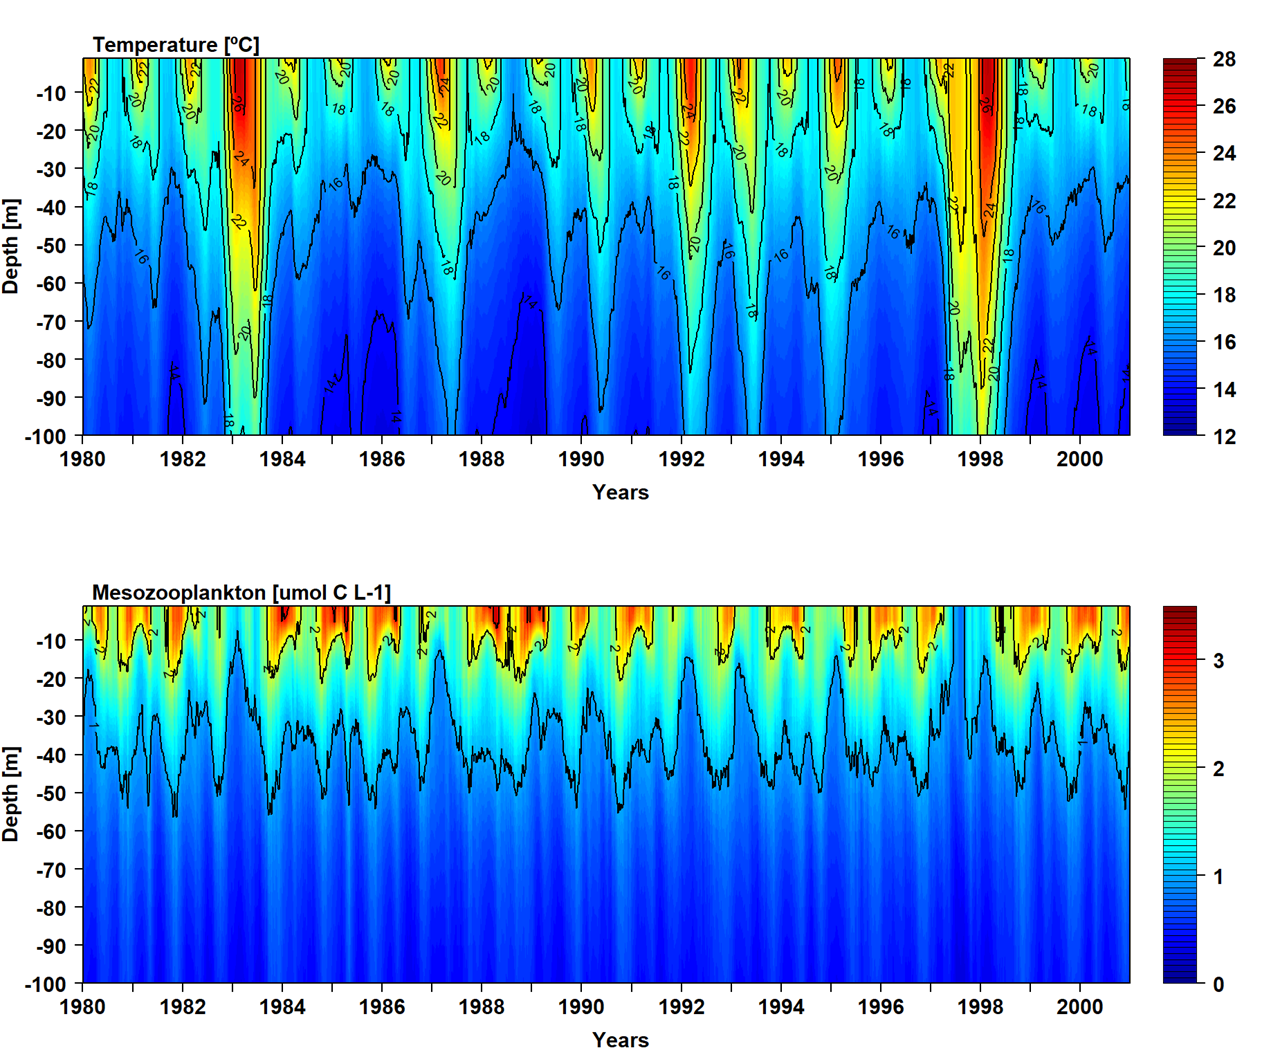
\includegraphics[width=1.0\textwidth]{figures/Chap3TempMesoInter.png}
	\centering
	\caption{Temperature (\textdegree C, upper panel) and mesozooplankton (umol, CL-1 bottom panel) vertical average from spawning zone of used as forcing for the interannual simulations of Peruvian anchovy recruitment.}
	\label{Chap3TempMesoInter}
\end{figure}

Figure \ref{Chap3CT_Depth_f_Inter} illustrates the impact of temperature and food on the growth of individuals, employing temperature correction curves (Cases 1 and 2) and a functional response for food concentration. A high value of the temperature correction implies a faster metabolism, while values close to zero are unfavorable for individuals. In Case 1, when the metabolism rate reaches a maximum at 19 \textdegree C, the negative effect during El Niño events is evident, extending to 80 meters depth (Fig. \ref{Chap3CT_Depth_f_Inter}, upper panel). Conversely, in Case 2 (when the metabolic rate reaches a maximum at 23 \textdegree C), this negative effect was concentrated in the first 45 meters depth (Fig. \ref{Chap3CT_Depth_f_Inter}, middle panel). Furthermore, Case 1 demonstrated a more frequent unfavorable effect during the study period (1980-2000) than Case 2. Finally, we observed that the value of the functional response, which limits the assimilation of individuals, remained at values of 0.5 (between 0 - 20 $m$) with the exception of extreme events where much lower values were observed, indicating a feeding deficiency (Fig. \ref{Chap3CT_Depth_f_Inter}, lower panel).\\

Fig. \ref{Chap3RecruitCase1Case2Inter} shows the difference between recruitment rates for Case 1 ($Sim 9$) and Case 2 ($Sim 10$). Both simulations show a decrease in recruitment rates during extreme events, however, Case 1 is more evident. Case 2 showed a favorable effect in the previous year to the extreme event, but then a decline in recruitment rates especially at the beginning of year 1998.\\

Analyses of variance (ANOVA) for $Sim 9$ (Case 1, Table \ref{Chap3ANOVAsim9}) and $Sim 10$ (Case 2, Table \ref{Chap3ANOVAsim10}) yielded comparable results. Spawning year accounted for 4.07 \% and 3.78 \%, respectively, while spawning month exhibited a relatively modest effect in Case 1 (0.39 \%) but a more pronounced one in Case 2 (3.55 \%). Spawning depth exhibited comparable and not dissimilar percentages of variance explanation (23.25 \% and 18.64 \%, respectively). Spawning bathymetry showed values of 4.70 \% and 7.56 \%, indicating a difference that was not as pronounced as that observed for spawning month. Finally, spawning latitude exhibited no significant difference between Case 1 and Case 2 (4.17 \% and 4.35 \%, respectively). The combinations of factors did not yield values that could be considered significant for differentiating Case 1 and Case 2 at the level of interannual simulations.\\

Given the importance of spawning depth for both simulations, it is necessary to consider the isolated effect of this factor. (Fig. \ref{Chap3RecruitCase1Case2InterDepths}) showed a high negative effect of extreme events on the three spawning depths in Case 1 ($Sim 9$, Fig. \ref{Chap3RecruitCase1Case2InterDepths}, left panels). This is less evident in Case 2 (($Sim 10$, Fig. \ref{Chap3RecruitCase1Case2InterDepths}, right panels)), where even in the shallowest depth (0-15 m), a favorability was observed before the onset of the extreme event. In the middle depth zone (15- 30 m) a negative effect of extreme events was observed, but then in the deeper zone (30 - 45 m) this effect was difficult to notice.

\begin{figure}[H]
	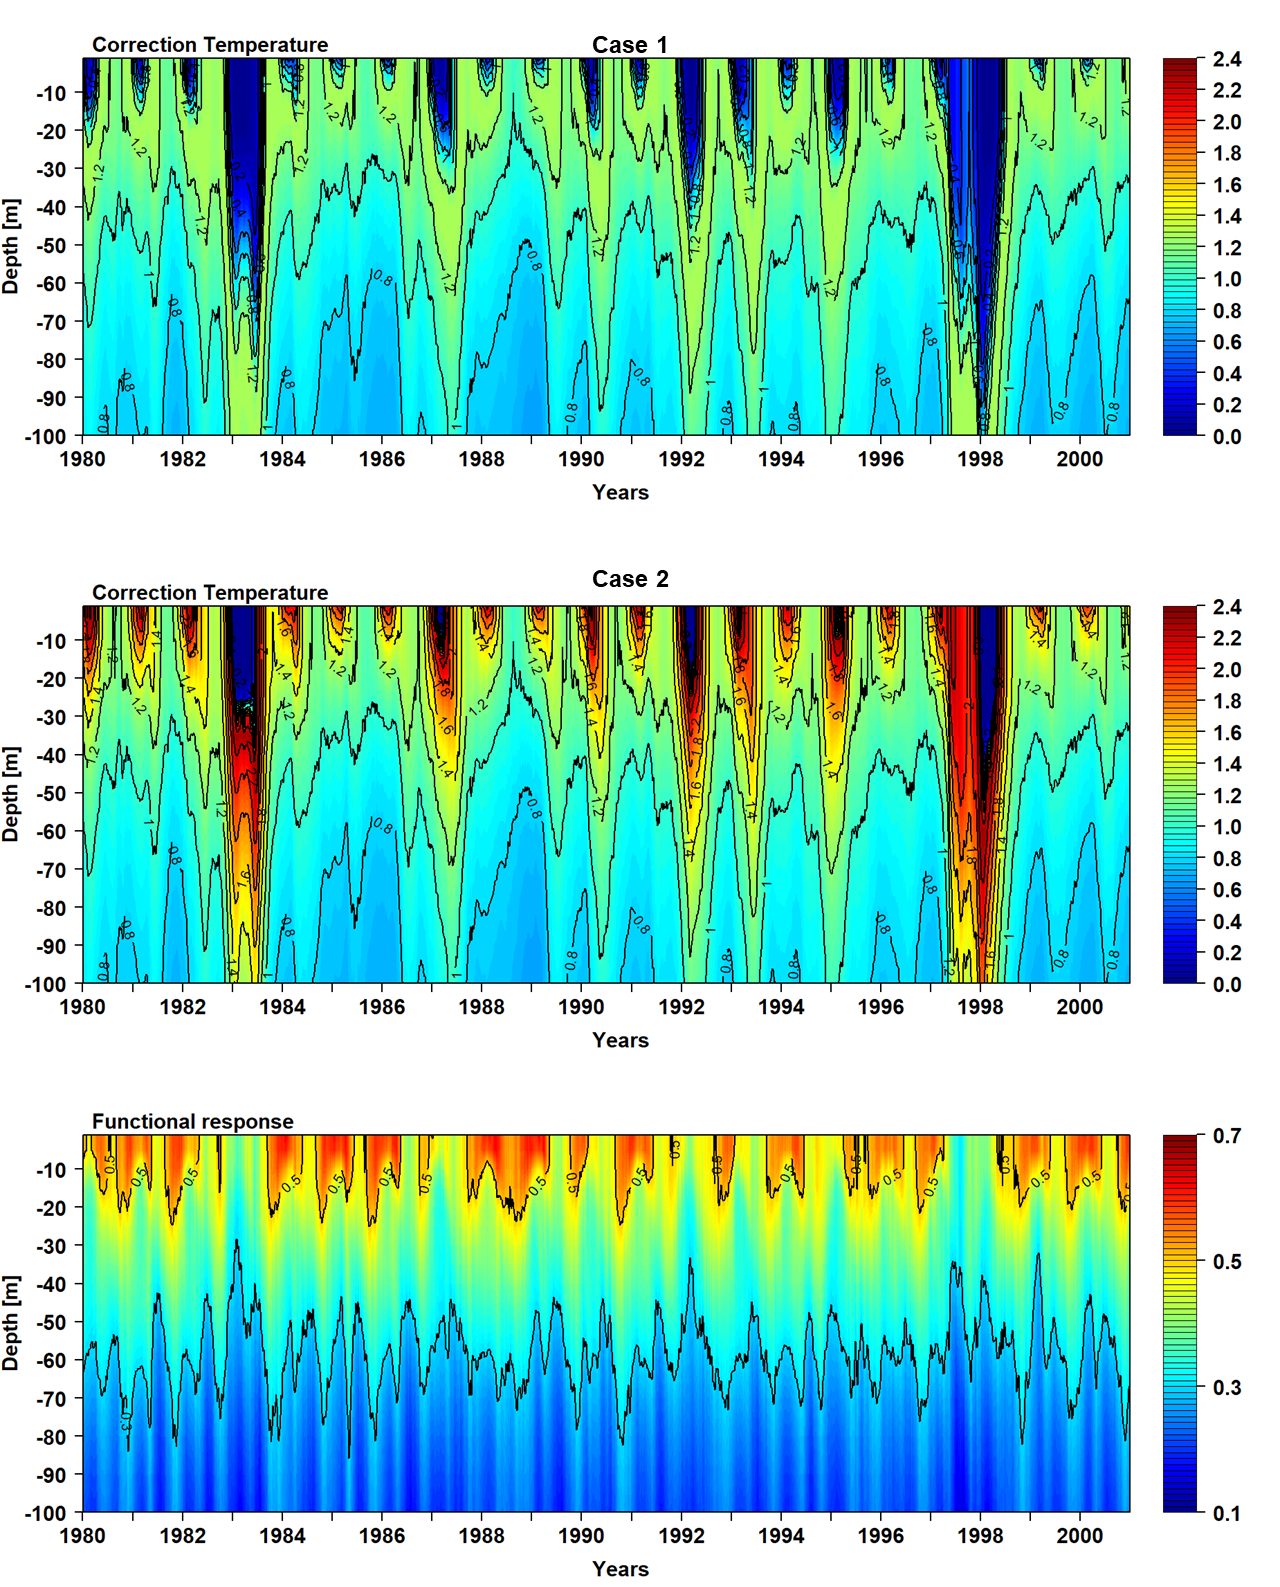
\includegraphics[width=1.0\textwidth]{figures/Chap3CT_Depth_f_Inter.png}
	\centering
	\caption{Spawning zone vertical average of temperature correction values for Case 1 (upper panel), Case 2 (middle panel) and the functional response for $K$ (half-saturation constant) fixed with a value of 1.6 (bottom panel).}
	\label{Chap3CT_Depth_f_Inter}
\end{figure}

\begin{figure}[H]
	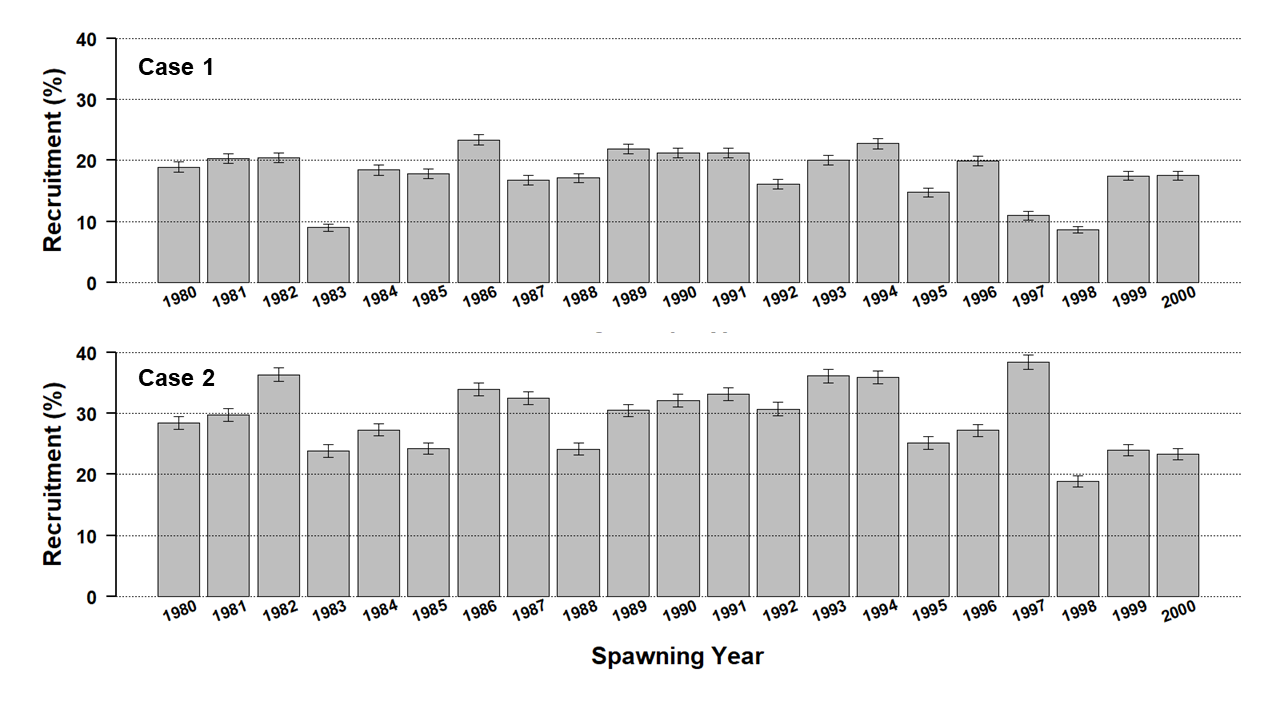
\includegraphics[width=1.0\textwidth]{figures/Chap3RecruitCase1Case2Inter.png}
	\centering
	\caption{Percentage of recruited larvae of Peruvian anchovy obtained from interannual simulation for Case 1 ($Sim 9$, upper panel) and Case 2 ($Sim 10$, bottom panel).}
	\label{Chap3RecruitCase1Case2Inter}
\end{figure}

%\begin{landscape}
\begin{table}[H]
\centering
\caption{ANOVA of recruitment rates for $Sim 9$ (Case 1).}
\rowcolors{1}{white}{gris}
\begin{adjustbox}{width=0.9\textwidth}
\small
\begin{tabular}{c|r|r|r|r|r|r}
\toprule
                                  &
	\textbf{Df}                   &
	\textbf{Sum Sq}               &
	\textbf{Mean Sq}              &
	\textbf{F-value}    		   &
	\textbf{Pr (\textgreater{F})} &
	$\mathbf{\% Exp}$      \\
\midrule
Year                  & 20	 & 845551.35  & 42277.57   & 258.49	   & 0	         & 4.07\\
Month                 & 11	 & 81363.69	  & 7396.70    & 45.22	   & 3.51E-99	 &0.39  \\
Depth                 & 2	 & 4830381.85 & 2415190.93 & 14766.83 & 0 			 & 23.25 \\
Bathymetry            & 2	 & 976098.17  & 488049.08  & 2984.00  & 0	         &4.70 \\
Latitude              & 8	 & 866683.05  & 108335.38  & 662.38	   & 0			 & 4.17\\
Year x Month          & 220 & 1011928.10 &	4599.67    & 28.12    & 0	         & 4.87  \\
Year x Depth          & 40	 & 268208.22  & 6705.21	   & 41.00	   & 3.1069e-313 & 1.29 \\
Year x Bathymetry     & 40  & 100511.81  & 2512.80	   & 15.36	   & 2.85E-103	 & 0.48 \\
Year x Latitude       & 160 & 779153.64  &	4869.71	   & 29.77	   & 0	         & 3.75  \\
Month x Depth         & 22	 & 392004.06  & 17818.37  &108.94	   & 0	         & 1.89 \\
Month x Bathymetry    & 22	 & 77401.74	  & 3518.26	   &21.51	   & 7.35E-86	 & 0.37  \\
Month x Latitude      & 88	 & 903658.26  & 10268.84  & 62.79	   & 0	         & 4.35  \\
Depth x Bathymetry    & 4	 & 64586.37	  & 16146.59   &98.72	   & 7.45E-84	 & 0.31  \\
Depth x Latitude      & 16	 & 358956.59  & 22434.79  & 137.17	   & 0	         &1.73 \\
Bathymetry x Latitude & 12	 & 794674.55  & 66222.88  & 404.90	   & 0	         & 3.83  \\
Residuals             & 51490	& 8421456.73 &163.56  & & 						 & 40.54\\
\bottomrule
\end{tabular}
\end{adjustbox}
\label{Chap3ANOVAsim9}
\end{table}
%\end{landscape}

%\begin{landscape}
\begin{table}[H]
\centering
\caption{ANOVA of recruitment rates for $Sim 10$ (Case 2).}
\rowcolors{1}{white}{gris}
\begin{adjustbox}{width=0.9\textwidth}
\small
\begin{tabular}{c|r|r|r|r|r|r}
\toprule
                                  &
	\textbf{Df}                   &
	\textbf{Sum Sq}               &
	\textbf{Mean Sq}              &
	\textbf{F-value}    		   &
	\textbf{Pr (\textgreater{F})} &
	$\mathbf{\% Exp}$      \\
\midrule
Year                  & 20    & 1391210.69  & 69560.53   & 265.92   & 0                   & 3.78  \\
Month                 & 11    & 1306548.20  & 118777.11  & 454.06   & 0                   & 3.55  \\
Depth                 & 2     & 6854738.93  & 3427369.47 & 13102.18 & 0                   & 18.64 \\
Bathymetry            & 2     & 2780996.10  & 1390498.05 & 5315.61  & 0                   & 7.56  \\
Latitude              & 8     & 1601243.32  & 200155.41  & 765.16   & 0                   & 4.35  \\
Year x Month          & 220   & 2136202.06  & 9710.01    & 37.12    & 0                   & 5.81  \\
Year x Depth          & 40    & 234791.26   & 5869.78    & 22.44    & 9.10E-161           & 0.64  \\
Year x Bathymetry     & 40    & 191622.73   & 4790.57    & 18.31    & 3.88E-127           & 0.52  \\
Year x Latitude       & 160   & 1626858.91  & 10167.87   & 38.87    & 0                   & 4.42  \\
Month x Depth         & 22    & 1221642.66  & 55529.21   & 212.28   & 0                   & 3.32  \\
Month x Bathymetry    & 22    & 162392.80   & 7381.49    & 28.22    & 2.11E-116           & 0.44  \\
Month x Latitude      & 88    & 1064069.64  & 12091.70   & 46.22    & 0                   & 2.89  \\
Depth x Bathymetry    & 4     & 95138.41    & 23784.60   & 90.92    & 3.64E-77            & 0.26  \\
Depth x Latitude      & 16    & 1033328.18  & 64583.01   & 246.89   & 0                   & 2.81  \\
Bathymetry x Latitude & 12    & 1610910.69  & 134242.56  & 513.18   & 0                   & 4.38  \\
Residuals             & 51487 & 13468365.16 & 261.59     &          &                     & 36.62 \\
\bottomrule
\end{tabular}
\end{adjustbox}
\label{Chap3ANOVAsim10}
\end{table}
%\end{landscape}

\begin{figure}[ht]
	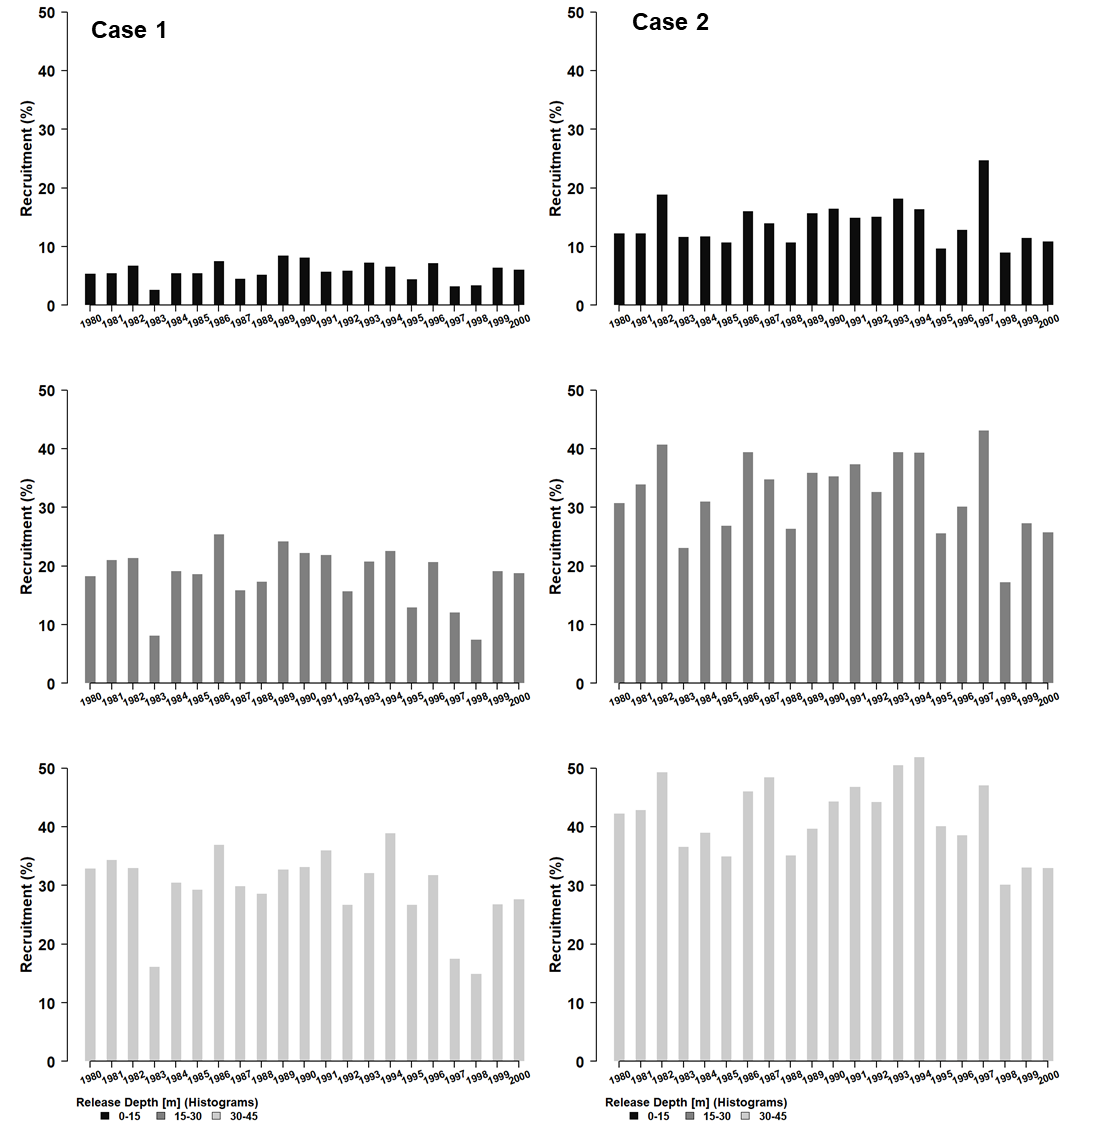
\includegraphics[width=1.0\textwidth]{figures/Chap3RecruitCase1Case2InterDepths.png}
	\centering
	\caption{Percentage of recruited larvae of Peruvian anchovy obtained from different spawning depths on the interannual simulation for Case 1 (left panels) and Case 2 (right panel).}
	\label{Chap3RecruitCase1Case2InterDepths}
\end{figure}

\clearpage
\section{Discussion of climatological simulations}\label{Chap3Disc1}

We studied larval retention and growth of the Peruvian anchovy (\textit{\gls{ringens}}) in the \acrshort{nhcs} using a biophysical model. This model was first forced by currents from a more modern configuration of a hydrodynamic model used previously at the same horizontal resolution (10 km; \cite{BrocLett2008}). We were able to replicate the general modeled patterns of larval retention obtained previously. Indeed, our results were consistent with another study aiming at answering the same scientific question but using a different dataset, thus proving the replicability of these results \citep{NAP25303}. This emphasis the robustness of the results despite the stochastic variability inherent to hydrodynamic model configurations. It was also crucial to replicate previous results before assessing the effects of new forcing products and other model components in order to avoid generating false conclusions \citep{Bake2016}. Here, in particular, we found the same opposite seasonal pattern relative to spawning depth (Fig. \ref{Chap3BrocVSFloreBarplots}) as \cite{BrocLett2008}. However, we obtained slightly higher coastal retention values during summer months for the three spawning depths considered. This result could be due to a greater stratification of the water column and to a higher spatial resolution of the wind stress forcing (weaker at the coast) in the new hydrodynamic simulations compared to the old one. Retention within the most coastal spawning zone (bathymetry 0 -100 $m$) was up to 20 \% higher in summer than in \cite{BrocLett2008}.\\

After including larval growth into our model based on the DEB theory, we explored simulations using a size criterion for retention (Fig. \ref{Chap3Case1CriterionCompar} and Fig. \ref{Chap3Case2CriterionCompar}), as opposed to an age criterion as before. Using a size criterion for retention means considering the impact of environmental variability on the planktonic life duration (\acrshort{pld}), which is crucial in biophysical modelling studies \citep{LettAyat2010}. Indeed, a shorter \acrshort{pld}, resulting from faster growth, is expected to increase local retention and therefore recruitment. Larvae that grow quicker may also escape predators, swim more efficiently and have therefore a better chance to survive \citep{Houd2008}, which was also explored in our results including mortality. In our simulations, larvae experienced temperatures ranging from $\sim$17\textdegree C in winter to $\sim$23\textdegree C in summer. The effect of temperature on growth depended on the hypothesis we made on the $C_T$ function (Eqn. \ref{C_T}) as we considered two temperature correction curves. Under the hypothesis of a max $C_T$ at $\sim$23.4\textdegree C (Case 1), the \acrshort{pld} could be as low as 20 days and the largest recruitment was found in summer in the Guayaquil Bay. However, this bay lies at the northern limit of \textit{\gls{ringens}} distribution \citep{CaldAyor2020}, and large recruitment of Peruvian anchovy has not been observed there to our knowledge. Tuning model parameters in order to fit a known distribution is a way to study the ecological niche limits. For our model prediction to fit the spatial extent of the observed spawning area (thus excluding the Guayaquil Bay, Fig. \ref{Chap3DistPartiMapEgg}e), we had to change the $C_T$ function such that its maximum value occurs at $\sim$19\textdegree C. In this case the average \acrshort{pld} of simulated recruited larvae was $\sim$50 days, which is in the order of in situ and laboratory observations \citep{PaloMuck1987}. Furthermore, \citep{CastPena2022} showed that the main habitat temperature range of adult anchovy population was 16-24\textdegree C, which is consistent with an optimal larval growth temperature around the middle of this range. However, the hypothesis that temperature would be the main factor limiting larval growth for individuals in the Guayaquil Bay should be challenged by new laboratory experiments designed to identify the upper temperature limit for larval growth. Indeed, current experiments found the fastest growth at 19\textdegree C for larval stages but did not investigate higher temperature values \citep{RiouOfel2021}. Some preliminary results tend to indicate for juvenile stages reduction of ingestion rate from 21\textdegree C (unpublished data), which would impact the growth rate. So, more laboratory experiments should be designed specifically to identify the shape of the $C_T$ function for \textit{\gls{ringens}}. Our results obtained with a 19\textdegree C maximum $C_T$ (Case 1) are also in line with \cite{XuChai2013} who found a rather adverse effect of inter-annual variability, specifically during the El Niño period, where the number of days to reach recruitment increased and survival decreased considerably.\\

In simulations where food was considered as not limiting larval growth, we found similar results as in simulations where both food and temperature were limiting. This result contrasts with \cite{ThomDuma2016} who used a similar bio-energetic approach as ours to study oyster larvae growth and recruitment in Polynesia. In a context where temperature variability was much smaller ($\sim$28-29\textdegree C) they found that food limitation explained most of recruitment variability. In our case, larval food limitation did not impact the seasonal pattern but it had a small impact on the spatial pattern, suggesting an average higher food limitation south of the Pisco upwelling cell ($\sim$14 – 15 \textdegree S), which is in line with a lower upwelling productivity \citep{EspiEche2017}.\\

The confirmation by laboratory experiments of a ``smooth” temperature correction function (as in Case 1 of the present simulations) for \textit{\gls{ringens}} would be consistent with the widely accepted idea that temperature is a limiting factor for anchovy blooming \citep{ChavBert2008}. However, a steeper temperature correction (Case 2) function would challenge this idea. In this latter case, other factors responsible for the northern limit of \textit{\gls{ringens}} habitat, possibly correlated with temperature, should be identified, as water masses \citep{BertSegu2004,SwarBert2008}, oxygen \citep{BertChai2011}, or food quality \citep{AyonSwar2008,CaldAyor2020} as food abundance was not found as a key limiting factor in our study. The change in species dominance shown in sediment records, corresponding to periods of environmental changes \citep{SalvField2018,SalvGuti2019}, would then be more associated to changes in stratification and circulation leading to a decrease in oxygen availability and/or decrease in ichthyoplankton retention \citep{BrocEche2013,EspiEche2021}, affecting larval vertical distribution.\\

In Peru, small pelagic fish monitoring is based on spawning biomass estimation and egg and larvae surveys \citep{PaulSori1987,Ayon2000,GutiCast2012} without explicitly accounting for spatial features (e.g. cross-shore and vertical). However, our results shows that spatial and vertical distribution also largely impact the success of recruitment. We suggest this information should be included in coupled model and observation operational system, which allows to forecast the seasonal success of recruitment. Thus, spatial monitoring of ichthyoplankton distribution should include assessment of vertical distribution. This can be achieved using multinet or, for a faster processing of the information, in situ imaging system that may allow a rapid processing \citep{OrenRate2020}.

\clearpage
\section{Discussion of interannual simulations}\label{Chap3Disc2}

The biogeochemical model represented well the most important features relatives to increase of temperature as showed by \citep{ColaCape2008} and decrease of anchovy prey \citep{AyonSwar2011} during the extreme El Nino events. The combination of high temperatures and little food during the extreme events generated a considerable decrease in recruitment rates in Case 1. This was not as evident in Case 2, in which, because the optimum temperature threshold is higher than in Case 1, recruitment was favored at the beginning of the temperature increase period, but then a negative effect followed due to the long duration of the temperature increase.\\

The results of Case 1 interannual recruitment rates coincide with those found by \cite{XuChai2013} with a considerable decrease of recruitment during El Nino events although they used a size recruitment criterion higher than the 2 cm, as was used in the present study. This was not as evident for Case 2.\\

It should also be noted that spawning depth had a greater effect in Case 1, affecting recruitment rates during El Nino events at all 3 depths. This characteristic was not very pronounced in Case 2, suggesting that Case 1 better represented the thermal limit of the Peruvian anchovy, however, this hypothesis has yet to be demonstrated by laboratory experiments.\\

The presence of prolonged periods of unfavorable conditions for the species during El Nino events also raises a migration behavior hypothesis of the Peruvian anchovy during its juvenile/adult phase, something that could be evaluated with another modelling tool \citep{BrocAuge2018} which includes a full life cycle model and swimming ability and was successfully applied in the ecosystem of the west coast of Africa. Another possible explanation would be the deeper vertical migration of the species, but due to the long duration of El Niño events, this would only allow it to escape unfavorable conditions for a short time, having to look for more favorable areas afterwards.\\

It should also be noted that in all experiments were assumed to have a uniform spawning, something that in reality depends on the variability of the spawning biomass \citep{CahuCubi2009} and should be taken into account for further studies.

\clearpage

\chapter{Dynamic Energy Budget model for \textit{Engraulis ringens}}\label{Chap4}

\section{Introduction}\label{Chap4Intro}

Dynamic Energy Budget (DEB) is a biological theory which takes individuals as dynamic systems, considered as the basic level of metabolic organization, relatively easy to make energy and mass balances. This theoretical framework allows us to model the allocation of energy and nutrients in living organisms through its entire life cycle \citep{Kooi2009}, using theoretical assumptions that have remained valid during its 40 years of development \citep{Kooi2020} making it comparable to other approaches in the goal of understanding how an individual and the surrounding environment interact.\\

This theory is particularly popular in ecophysiology and population ecology, where it helps scientists understand how organisms allocate their energy and resources to various life processes, such as growth, maintenance, and reproduction. The DEB theory is based on a set of mathematical equations and concepts that describe how an organism acquires, uses, and allocates energy. These equations take into account factors like energy acquisition (feeding), energy storage, and the trade-offs between various life processes inside the individual. Different individuals (species), present differences that are captured by the DEB theory at the level of their parameter values \citep{Meer2006}. In this way, this theory helps us to understand how a species can flourish or decline, how it competes for resources or how it adapts in different environmental conditions.\\

The strategy is to start from mechanistic considerations at the individual level incorporating details about the physiology of the species defining parameters that describe how the organism acquires, allocates, and uses energy \citep{KooiSabe1986}. These parameters include assimilation rates, growth rates, reproduction rates, maintenance costs, and more, all of which are typically influenced by factors like temperature, food availability, and age, cementing the basic blocks to model studies on \textit{Engraulis ringens} structured population.\\

\textit{E. ringens}, commonly known as the Peruvian anchovy, is a small pelagic fish species found in the southeastern Pacific Ocean along the coasts of South America, particularly in the Humboldt Current system \citep{GutiSwar2007}. Along with the Peruvian anchovy, there is usually an important presence of sardine (\textit{Sardinops sagax}), another small pelagic species, but since the decade of the 2000s, there have been no significant landings off the peruvian coast \citep{CardFran2015}, and the fact that \textit{E. ringens} is usually associated with the coastal zone while sardines occupy more oceanic areas due to different feeding and oxygen conditions \citep{EspiBert2008,BertChai2011}, we can study the interaction of anchovy with their environment without considering a competition with sardines.\\

When commercially targeted marine fish feed on phytoplankton and zooplankton, they assimilate and redistribute essential nutrients, influencing the productivity and structure of the ecosystem \citep{LeMeGuie2022}. Also, anchovies help maintain the balance and stability of marine ecosystems due their population dynamics can impact the abundance of other species, influencing ecosystem health and resilience to environmental changes \citep{FennSear2023}. Since Dynamic Energy Budget theory can be used in IBM models, ecosystem models, toxicology models \citep{LavaFilg2021}, a DEB model for \textit{E. ringens} is essential for future ecological studies and for conservation purposes.

Below, we list some important concepts in DEB modelling:

\begin{itemize}
%  \centering
  \item Energy Budget: DEB modeling starts by quantifying the energy fluxes into and out of an organism. This includes energy gained through feeding, losses due to metabolism and maintenance, growth, reproduction, and other processes.\\
  
  \item Allocation and Utilization: The model describes how the acquired energy is allocated and utilized for different biological processes, such as growth, reproduction, and maintenance. It helps to understand how organisms prioritize energy allocation under varying conditions.\\

  \item Reserves and Structure: DEB models account for the storage of surplus energy as reserves (e.g., fat, proteins) and the development of structural components (e.g., organs, tissues). The dynamics of these reserves are critical in understanding an organism's life history.\\

  \item Maintenance and Maturation: DEB models consider the energy spent on maintaining basic bodily functions (maintenance) and the energy used for growth and development (maturation) at different life stages.\\

  \item Environmental Factors: The model incorporates two principal environmental factors like temperature, food availability, and other abiotic factors (not taken into account in this study) to assess their influence on energy acquisition, utilization, and allocation.\\

\end{itemize}

In addition, we present a list of potential uses of a DEB model:

\begin{itemize}
%  \centering
  \item Growth and Development: DEB models provide insights into the growth patterns and development stages of organisms. They help predict how growth rates vary with environmental conditions and resource availability.\\
  
  \item Reproduction and Life History Strategies: DEB models enable the study of reproductive strategies, including the timing and allocation of energy to reproduction. This aids in understanding reproductive trade-offs and strategies for optimizing its survival.\\
  
  \item 	Responses to Environmental Change: DEB models help predict how organisms respond to changes in environmental conditions, such as temperature, nutrient availability, and pollution. This is crucial for assessing the impacts of climate change and other environmental stressors.\\
  
  \item Optimizing Fisheries and Aquaculture: DEB models aid in optimizing fisheries and aquaculture practices by predicting growth rates, maturation, and reproduction, leading to sustainable management of fish stocks.\\
  
  \item Toxicology and Ecotoxicology: Although it is not the objective of this study, DEB models can be applied to assess the effects of toxins and pollutants on an organism's energy allocation and life history traits, aiding in understanding toxicological impacts.\\

\end{itemize}

So, in this chapter, we will start by showing the available data collection, the calibration of a DEB model with growth acceleration during its early life stages (that was not taken into account in the Chapter \ref{Chap3}) and its implementation in the IBM called Ichthyop-DEB model, to explore the interaction of the species with its environment, focusing mainly on its food demand since the effect of temperature has been well documented previously.

\section{Methods}\label{Chap4Meth}

\subsection{Data collection}\label{Chap4MethDat}

A model is composed of mathematical equations that represent the characteristics of a dynamic system. These equations include parameters that allow the comparison of different systems, and these parameters are estimated from empirical data \citep{RaolGiri2004}. Gather empirical data and literature data related to \textit{E. ringens}, includes growth rates, especially in their early stages of life, reproduction rates, feeding rates, body sizes, and any other relevant biological measurements.\\

In spite of the application of DEB theory is challenging because the state variables and parameters are abstract quantities that are not directly observable, the parameter estimation method \citep{Lika2011a,Lika2011b} makes use of different data sources.\\

However, there are different levels of difficulty in collecting individual or population data for a species. For example, a collection of population data for \textit{E. ringens} is well described by \citep{MarzShin2009}, but data on metabolic rates, feeding rates or vertical behaviour (characteristics that require captive breeding) have been studied more in other similar species and other ecosystems \citep{AldaCota2008,CermUria2003,KramZwei1968,DetwHoud1970,Hunt1971,Hunt1984,SakaKimu1976,Houd1977,MethKram1979,Thei1980,Brow1983}, while laboratory rearing (especially for early life stages) is just beginning for \textit{E. ringens} \citep{RiouOfel2021,OfelMoya2023}, difficulty in rearing, which can be explained by the high migratory behaviour of anchovies in general \citep{OlivSala2001,MoraBaba2010,TanaOhsh2010,PoliHure2015,GuraFach2017,CastNiqu2021}.\\

The following is a description of the available and preferably most updated data used for DEB parameters estimation on \textit{E. ringens}.\\

\subsection{Parameter estimation}

Estimating parameters for a Dynamic Energy Budget (DEB) model involves a process to fit the model to empirical data, allowing it to accurately represent the energy allocation and life history of a specific organism, in this case, \textit{E. ringens}.\\

We used a bivariate statistical technique \citep{Lika2011a,Lika2011b} to estimate the values of the model parameters that minimize the difference between model predictions and observed data. Then, we fitted the DEB model to the compiled empirical data, adjusting parameters to best represent the biological processes and energy dynamics of \textit{E. ringens}.\\

In order to show the difference between the DEB-standard model (\textit{E. encracicolus}) used in Chapter \ref{Chap3}, a comparative table with the estimated parameters for \textit{E. ringens} is presented below.

Table 1: Parameters used for the bioenergetic model describing larval growth. These values were estimated by Pethybridge et al. (2013) for Engraulis encrasicolus and compared with the parameters estimated for E. ringens (current study). The values of $T_L$, $T_H$, $T_AL$, $T_AH$ are detailed for case 1. Values for case 2 are indicated in parenthesis when different from case 1.

\begin{figure}[ht]
	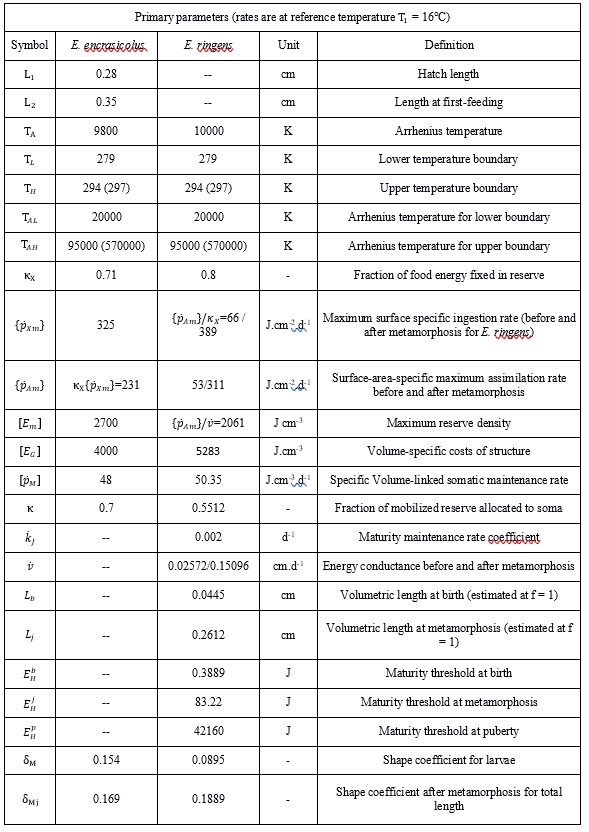
\includegraphics[width=1.0\textwidth]{figures/tablepars.png}
	\centering
	%\caption{Temperature correction curves for the metabolic flux in the dynamic energy budget model \textcolor{red}{(equation 5), revisar la ref cruzada}; blue and red curve correspond respectively to case 1 and case 2 in Table 1.}
%	\label{Fig3_02}
\end{figure}

%\begin{table}[]
%\begin{tabular}{lllll}
%\multicolumn{5}{l}{\textbf{Primary parameters (rates are at reference temperature T\_1 = 16°C)}} \\
%\textbf{Symbol} &
%  \textbf{\textit{E. encrasicolus}} &
%  \textbf{\textit{E. ringens}} &
%  \textbf{Unit} &
%  \textbf{Definition} \\
%L\_1                    & 0.28           & --                    & cm     & Hatch length                                            \\
%L\_2                    & 0.35           & --                    & cm     & Length at first-feeding                                 \\
%T\_A                    & 9800           & 10000                 & K      & Arrhenius temperature                                   \\
%T\_L                    & 279            & 279                   & K      & Lower temperature boundary                              \\
%T\_H                    & 294 (297)      & 294 (297)             & K      & Upper temperature boundary                              \\
%T\_AL                   & 20000          & 20000                 & K      & Arrhenius temperature for lower boundary                \\
%T\_AH                   & 95000 (570000) & 95000 (570000)        & K      & Arrhenius temperature for upper boundary                \\
%κ\_X                    & 0.71           & 0.8                   & -      & Fraction of food energy fixed in reserve                \\
%\{p ̇\_Xm \} &
%  325 &
%  \{p ̇\_Am \}/κ\_X=66 / 389 &
%  J.cm-2.d-1 &
%  Maximum surface specific ingestion rate (before and after metamorphosis for E. ringens) \\
%\{p ̇\_Am \} &
%  κ\_X \{p ̇\_Xm \}=231 &
%  53/311 &
%  J.cm-2.d-1 &
%  Surface-area-specific maximum assimilation rate before and after metamorphosis \\
%{[}E\_m {]}             & 2700           & \{p ̇\_Am \}/v ̇=2061 & J cm-3 & Maximum reserve density                                 \\
%{[}E\_G {]}             & 4000           & 5283                  & J.cm-3 & Volume-specific costs of structure                      \\
%κ                       & 0.7            & 0.5512                & -      & Fraction of mobilized reserve allocated to soma         \\
%k ̇\_J                  & --             & 0.002                 & d-1    & Maturity maintenance rate coefficient                   \\
%v ̇                     & --             & 0.02572/0.15096       & cm.d-1 & Energy conductance before and after metamorphosis       \\
%L\_b                    & --             & 0.0445                & cm     & Volumetric length at birth (estimated at f = 1)         \\
%L\_j                    & --             & 0.2612                & cm     & Volumetric length at metamorphosis (estimated at f = 1) \\
%E\_H\textasciicircum{}b & --             & 0.3889                & J      & Maturity threshold at birth                             \\
%E\_H\textasciicircum{}j & --             & 83.22                 & J      & Maturity threshold at metamorphosis                     \\
%E\_H\textasciicircum{}p & --             & 42160                 & J      & Maturity threshold at puberty                           \\
%δ\_M                    & 0.154          & 0.0895                & -      & Shape coefficient for larvae                            \\
%δ\_Mj                   & 0.169          & 0.1889                & -      & Shape coefficient after metamorphosis for total length  \\
%                        &                &                       &        &                                                        
%\end{tabular}
%\end{table}


\chapter{General discussion and conclusions}\label{Chap5}

Then, the aims of this chapter/article/paper is to produce the first \acrshort{deb} model for Peruvian anchovy (\textit{\gls{ringens}}),  with a specific set of parameters estimated  that includes growth acceleration ($DEB_{abj}$)  during the larval period to metamorphosis.% and to compare the patterns of larval recruitment with  a previous growth model implemented by \citep{FlorLett2023} using an \gls{ich-deb} model and highlight its differences from the standard version ($DEB_{std}$).\\

\clearpage
\section{Discusión general}
El reclutamiento de un individuo en una población sigue siendo uno de los mayores misterios de las ciencias marinas, más aún cuando el concepto mismo de reclutamiento está en discusión y hasta es específico de cada especie (Miller et al. 1988), pero lo que es cierto para todas las especies, es que el reclutamiento está íntegramente ligado a la biomasa desovante (Cole and McGlade 1998) y las condiciones ambientales (Roy et al. 1992) que actúan a través de un amplio rango de estadios de vida.\\

Más allá de una definición universal de reclutamiento, nos hemos enfocado en comprender el mecanismo con el que un individuo interactúa con su ambiente, cómo este afecta su desarrollo a través de su ciclo de vida y cómo promueve/limita el éxito de reclutamiento. Es por ello que el objetivo general de esta tesis es desarrollar un modelo mecanístico que una el conocimiento de la variabilidad ambiental y el efecto directo sobre los estadios de vida temprana de la anchoveta Peruana (Engraulis ringens), siendo extensible esta técnica a otras especies de peces o recursos marinos de interés.\\

Por practicidad, hemos denominado “reclutamiento larval”, o simplemente “reclutamiento” a procesos ligados al transporte y crecimiento larval, procesos derivados de las corrientes oceánicas, la temperatura y la disponibilidad de alimento. Con todos estos elementos, hemos desarrollado una herramienta lagrangiana, denominada Ichthyop-DEB, con la capacidad hacer el seguimiento individual en el desarrollo de individuos de E. ringens hasta alcanzar el éxito de reclutamiento larval, limitándose a simular el movimiento pasivo de cada individuo.\\

Ichthyop-DEB nos permite definir zonas de desove que pueden ser divididas horizontal y verticalmente, desde las cuales los individuos son liberados (desovados) aleatoriamente iniciando su proceso de deriva y/o desarrollo (crecimiento). Luego, sólo los individuos que cumplan con ciertos criterios serán aquellos que alcancen el éxito de reclutamiento. Ichthyop-DEB nos ofrece la opción de elegir hasta tres criterios de reclutamiento, dependiendo de la necesidad del usuario. El criterio 1, está ligado al transporte larval en función de las corrientes oceánicas y considerará como reclutados, sólo a aquellos individuos que al final de la simulación, estén dentro de la zona reclutamiento (zona también definida por el usuario). El criterio 2, agrega el proceso de crecimiento en longitud, simulado por un Modelo de Presupuesto Energético (DEB) para que el individuo alcance una talla mínima (2 cm para E. ringens) y que el individuo esté dentro de la zona de reclutamiento para considerarlo como reclutado. El criterio 3 es un procesamiento posterior a Ichthyop-DEB, del que utilizaremos una variable denominada “edad al reclutamiento”, edad que varía con cada individuo dependiendo las condiciones de temperatura y alimento. Así, un individuo que experimenta una mayor tasa de crecimiento reclutará más rápido y tendrá un “valor” superior que uno que recluta días después. Este “valor” es calculado en función de la edad de reclutamiento y una tasa de mortalidad diaria. De esta forma, Ichthyop-DEB puede ser entendida como una herramienta especializada en cuantificar el efecto del ambiente (corrientes oceánicas, temperatura y aimento) sobre los primeros estadios de vida temprana de organismos marinos durante su fase planktónica.\\

%Many studies focused on survival during the early life history stages, and the causal mechanisms and how impacts on subsequent recruitment. Of the various recruitment hypotheses, those regarding starvation can be addressed by the Ichthyop-DEB tool developed in this manuscript. For example, critical period hypothesis (Hjort 1914).\\
%
%One of the first questions we can ask ourselves when choosing a model to try to answer a scientific question is: Why trust this model? And furthermore, how complex does this model need to be? This will depend on the question, the scale of the process to be studied and the precedents of the answers to this question.\\
%
%for the most part of fisheries is how good is the recruitment of the species. This is already a complex process that includes different agents such as environmental conditions, the state of its adult population or its adaptive capacity.\\
% 
%In this context of study, the Peruvian anchovy has been well studied, from associating environmental variables to the presence of large schools at the time of fishing to having models with equations that describe how the environment impact the species at different levels as well as the frequency and detail of the monitoring system that is targeted each year. We have focused on the modeling approach.\\
%
%Here we present the development of a modeling tool that aims to understand the impact of temperature and food availability on recruitment and survival of early life stages of aquatic species through an individual-based modeling approach (Fig. 5.1). This approach was born from adding complexity to a larval dispersal model (Brochier et al. 2008; Lett et al. 2008) to which a module was added to simulate growth using a DEB bioenergetic model (Kooijman 2009). The results of the present study give robustness to previous results (Brochier et al. 2008) on larval retention patterns where we agree that spawning depth plays a very important role in addition to a seasonal variation that depends on depth. This is quite interesting considering that over the years new versions of the hydrodynamic model of coastal circulation off Peru have been created, and these updates have maintained the general patterns. (replicabilidad de resultados, ). We can conclude that to work on E. ringens recruitment simulations, in order to save computational time and energy, we can continue with a spatial resolution of 10 km. In addition, it is recommended to use the coastal behavior called standstill, since for the purposes of our research it will not significantly affect near-shore particle transport.\\
%
%In Peru, small pelagic fish monitoring is based on spawning biomass estimation and egg and larvae surveys (Pauly and Soriano 1987; Ayón 2000; Gutiérrez et al. 2012) without explicitly accounting for spatial features (e.g. cross-shore and vertical). However, our results shows that spatial and vertical distribution also largely impact the success of recruitment. We suggest this information should be included in coupled model and observation operational system, which allows to forecast the seasonal success of recruitment. Thus, spatial monitoring of ichthyoplankton distribution should include assessment of vertical distribution. This can be achieved using multinet or, for a faster processing of the information, in situ imaging system that may allow a rapid processing (Orenstein et al. 2020).\\
%
%Agragar a discusion
%
%¿What makes a late anchovy larva? The
%development of the caudal fin seen as a
%milestone in fish ontogeny?
%STYLIANOS SOMARAKIS1* AND NIKOLAOS NIKOLIOUDAKIS1,2 REVISAR
%
%From egg production to recruits: Connectivity and inter-annual
%variability in the recruitment patterns of European anchovy
%in the northwestern Mediterranean
%Andres Ospina-Alvarez
%
%Integration of bioenergetics in an individual-based model
%to hindcast anchovy dynamics in the Bay of Biscay
%Juan Bueno-Pardo
%
%The fisheries history of small pelagics in the Northern Mediterranean
%Elisabeth van Beveren
%
%Size, permeability and buoyancy of anchovy (Engraulis
%Encrasicolus) and sardine (Sardina Pilchardus) eggs in
%relation to their physical environment in the Bay of Biscay
%Huret
%
%Determinants of growth and selective mortality in anchovy and sardine in
%the Bay of Biscay
%Bo¨ens
%
%Comparing biological traits of anchovy and sardine in the Bay of Biscay: A modelling approach with the Dynamic Energy Budget
%Paul Gatti (1) 
%
%Modelling potential spawning habitat of sardine (Sardina pilchardus) and anchovy (Engraulis encrasicolus) in the Bay of Biscay
%Benjamin Planque (1) 
%
%Historical fluctuations in spawning location of anchovy (Engraulis encrasicolus) and sardine (Sardina pilchardus) in the Bay of Biscay during 1967?73 and 2000?2004
%Edwige Bellier (1)
%
%Characterising and comparing the spawning habitats of anchovy Engraulis encrasicolus and sardine Sardinops sagax in the southern Benguela upwelling ecosystem
%N. Twatwa ,

\backmatter
\chapter{General discussion and conclusions}\label{Chap6}

\clearpage

\section{Discussion}

The recruitment of an individual into a population remains one of the most perplexing enigmas of marine science, particularly when the very concept of recruitment is under discussion and even species-specific (Miller et al. 1988). However, it is evident that recruitment is inextricably linked to spawning biomass (Cole and McGlade 1998) and environmental conditions (Roy et al. 1992) across a wide range of life stages, a fact that is universally applicable to all species.\\

In addition to defining recruitment universally, we have concentrated on understanding the manner in which an individual interacts with its environment, the effects of this interaction on its development throughout its life cycle, and the ways in which it affects recruitment success. Therefore, the overarching objective of this thesis is to develop a mechanistic model that integrates the knowledge of environmental variability and the direct impact on the early life stages of the Peruvian anchoveta (Engraulis ringens). This technique can be extended to other fish species or marine resources of interest.\\

For the sake of practicality, we have designated the processes linked to larval transport and growth, which are influenced by ocean currents, temperature, and food availability, as "larval recruitment," or simply "recruitment." With these elements in mind, we have developed a Lagrangian tool, called Ichthyop-DEB, which is capable of tracking the development of individual E. ringens individuals until larval recruitment success is achieved. In our simulations, we limit ourselves to the passive movement of each individual.\\

The Ichthyop-DEB software enables the user to define spawning zones that can be divided horizontally and vertically. These zones can then be populated with individuals, which are randomly released (spawned) to initiate their drift and/or development (growth) process. Subsequently, only those individuals who meet the specified criteria will be considered successful in their recruitment. Ichthyop-DEB offers the option of selecting up to three recruitment criteria, contingent on the user's requirements. The first criterion is linked to larval transport according to ocean currents and considers only those individuals to be recruited who, at the conclusion of the simulation, are within the defined recruitment zone (also determined by the user). The second criterion adds the process of growth in length, simulated by an Energy Budget Model (EBM), so that the individual reaches a minimum length (2 cm for E. ringens) and is within the recruitment zone to be considered as recruited. The third criterion is a post-Ichthyop-DEB processing step. This criterion employs a variable called "age at recruitment," which varies with each individual in accordance with temperature and food conditions. Consequently, an individual that experiences a higher growth rate will recruit at a faster rate and will have a higher value than one that recruits days later. The value is calculated as a function of age at recruitment and a daily mortality rate. In this manner, Ichthyop-DEB can be regarded as a specialized tool for quantifying the impact of environmental factors (ocean currents, temperature, and food availability) on the early life stages of marine organisms during their planktonic phase.\\

Many studies focused on survival during the early life history stages, and the causal mechanisms and how impacts on subsequent recruitment. Of the various recruitment hypotheses, those regarding starvation can be addressed by the Ichthyop-DEB tool developed in this manuscript. For example, critical period hypothesis (Hjort 1914).\\

One of the first questions we can ask ourselves when choosing a model to try to answer a scientific question is: Why trust this model? And furthermore, how complex does this model need to be? This will depend on the question, the scale of the process to be studied and the precedents of the answers to this question. For the most part of fisheries is how good is the recruitment of the species. This is already a complex process that includes different agents such as environmental conditions, the state of its adult population or its adaptive capacity.\\

In this context of study, the Peruvian anchovy has been well studied, from associating environmental variables to the presence of large schools at the time of fishing to having models with equations that describe how the environment impact the species at different levels as well as the frequency and detail of the monitoring system that is targeted each year. We have focused on the modeling approach.\\

Here we present the development of a modeling tool that aims to understand the impact of temperature and food availability on recruitment and survival of early life stages of aquatic species through an individual-based modeling approach (Fig. 5.1). This approach was born from adding complexity to a larval dispersal model (Brochier et al. 2008; Lett et al. 2008) to which a module was added to simulate growth using a DEB bioenergetic model (Kooijman 2009). The results of the present study give robustness to previous results (Brochier et al. 2008) on larval retention patterns where we agree that spawning depth plays a very important role in addition to a seasonal variation that depends on depth. This is quite interesting considering that over the years new versions of the hydrodynamic model of coastal circulation off Peru have been created, and these updates have maintained the general patterns. (replicabilidad de resultados, ). We can conclude that to work on E. ringens recruitment simulations, in order to save computational time and energy, we can continue with a spatial resolution of 10 km. In addition, it is recommended to use the coastal behavior called standstill, since for the purposes of our research it will not significantly affect near-shore particle transport.\\

In Peru, small pelagic fish monitoring is based on spawning biomass estimation and egg and larvae surveys (Pauly and Soriano 1987; Ayón 2000; Gutiérrez et al. 2012) without explicitly accounting for spatial features (e.g. cross-shore and vertical). However, our results shows that spatial and vertical distribution also largely impact the success of recruitment. We suggest this information should be included in coupled model and observation operational system, which allows to forecast the seasonal success of recruitment. Thus, spatial monitoring of ichthyoplankton distribution should include assessment of vertical distribution. This can be achieved using multinet or, for a faster processing of the information, in situ imaging system that may allow a rapid processing (Orenstein et al. 2020).\\

Fish populations can vary greatly over time, from interannual to millennial fluctuations. For short-lived fish, these two scales of variability are comparable in magnitude, indicating that reproductive success and recruitment are the main factors contributing to abundance. Reproductive success refers to the number of offspring an individual produces per breeding event or over their lifetime, which is closely related to the environment in which the parents develop and is something that can be monitored through research cruises during the spawning season, and in the other hand to address the ``recruitment problem'', which is the lack of knowledge to explain recruitment variability, a solid theoretical basis and practical methods are necessary, however, monitoring early life stages in the natural environment is inherently difficult, posing a great challenge with more questions than answers.

Theories on how environmental conditions affect recruitment success, based on the survival/mortality of early life-history stages, can be categorized into mechanistic and synthesis theories. Mechanistic theories focus on particular physical processes, while synthesis theories aim to integrate the various mechanistic processes into a single conceptual framework. Although some theories have been successfully tested, there has been little success in reliably predicting recruitment success based on environmental conditions \citep{ColeMcGl1998}.

\section{Conclusions}

\clearpage

%¿What makes a late anchovy larva? The
%development of the caudal fin seen as a
%milestone in fish ontogeny?
%STYLIANOS SOMARAKIS1* AND NIKOLAOS NIKOLIOUDAKIS1,2 REVISAR
%
%From egg production to recruits: Connectivity and inter-annual
%variability in the recruitment patterns of European anchovy
%in the northwestern Mediterranean
%Andres Ospina-Alvarez
%
%Integration of bioenergetics in an individual-based model
%to hindcast anchovy dynamics in the Bay of Biscay
%Juan Bueno-Pardo
%
%The fisheries history of small pelagics in the Northern Mediterranean
%Elisabeth van Beveren
%
%Size, permeability and buoyancy of anchovy (Engraulis
%Encrasicolus) and sardine (Sardina Pilchardus) eggs in
%relation to their physical environment in the Bay of Biscay
%Huret
%
%Determinants of growth and selective mortality in anchovy and sardine in
%the Bay of Biscay
%Bo¨ens
%
%Comparing biological traits of anchovy and sardine in the Bay of Biscay: A modelling approach with the Dynamic Energy Budget
%Paul Gatti (1) 
%
%Modelling potential spawning habitat of sardine (Sardina pilchardus) and anchovy (Engraulis encrasicolus) in the Bay of Biscay
%Benjamin Planque (1) 
%
%Historical fluctuations in spawning location of anchovy (Engraulis encrasicolus) and sardine (Sardina pilchardus) in the Bay of Biscay during 1967?73 and 2000?2004
%Edwige Bellier (1)
%
%Characterising and comparing the spawning habitats of anchovy Engraulis encrasicolus and sardine Sardinops sagax in the southern Benguela upwelling ecosystem
%N. Twatwa ,
\nolinenumbers
%----- Print Bibliography -----%
\renewcommand\bibname{References}   % Change bibliography title.
\bibliographystyle{bst/authordate1} % Directory where the references are stored.
%\bibliographystyle{bst/authordate3}

%----- Format the bibliography using a smaller font size -----%
{\footnotesize \bibliography{bib/ThesisBib}}
%{\scriptsize \bibliography{bib/ThesisBib}}

%%----- Print glossary -----%
\printnoidxglossary

% Add appendix
\appendix
\chapter{Supplementary material}\label{App1}

\begin{figure}[ht]
	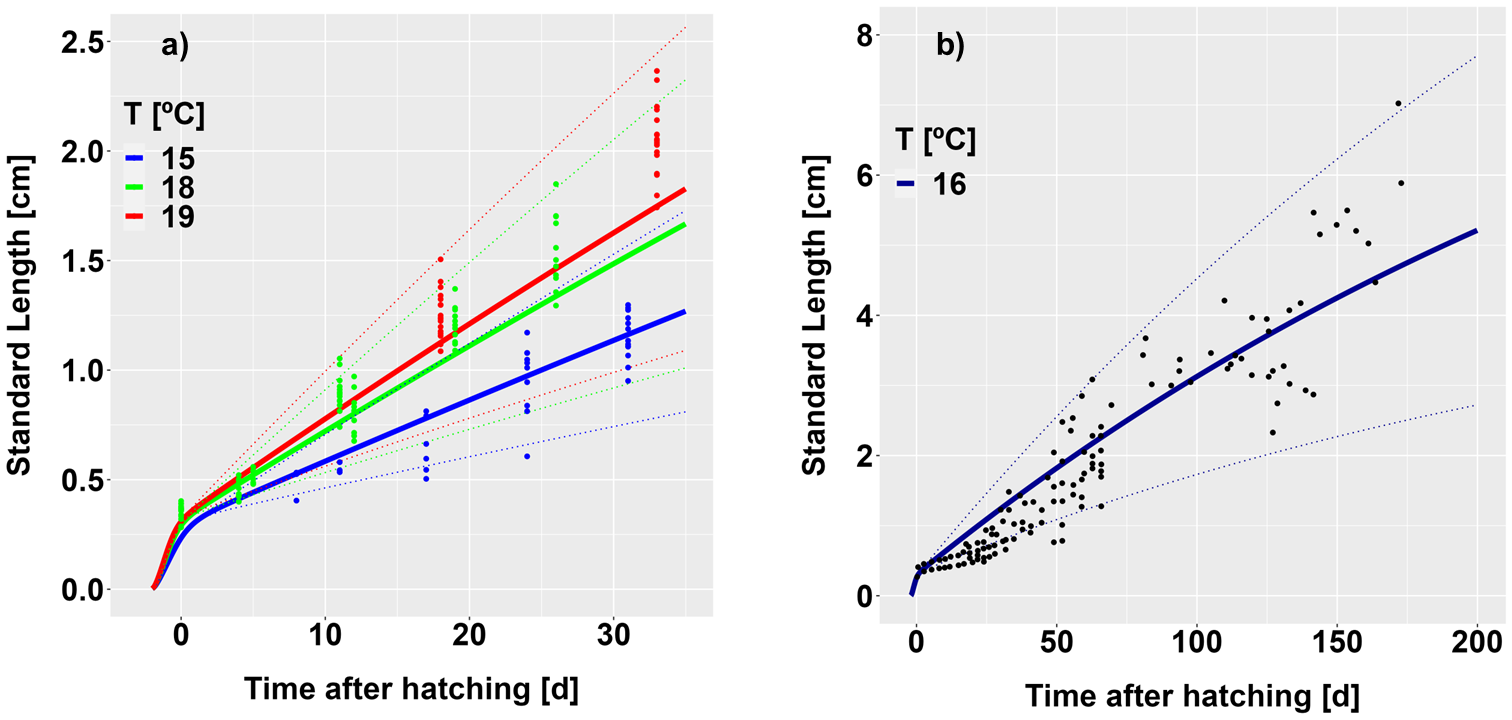
\includegraphics[width=1.0\textwidth]{figures/S1DEBvsData.png}
	\centering
	\caption{Comparison of Peruvian anchovy simulated larval growth and laboratory observations from \cite{RiouOfel2021} (a) and in situ observations from \cite{MoreClar2011} (b). Thick lines correspond to average size predictions considering ten $f$ values from 0.1 to 1 with 0.1 steps (food limitation factor, see section 2.1.6) at $19$\textdegree $C$ (red), $18$\textdegree $C$ (green) and $15$\textdegree $C$ (blue) in (a) and at $16$\textdegree C in (b). Dotted lines correspond to standard deviation of the simulated larval growth. Colored dots show the corresponding observations. The bioenergetic model parameters were taken from \cite{PethRoos2013}. Note that the scales are different in the two panels.}
	\label{S1DEBvsData}
\end{figure}

\section{Standard $\acrshort{deb}_{std}$ Equations in Ichthyop-DEB model}\label{DEBstdEqn}

Jorge Flores-Valiente et al.\\

The following description is a simplification of the \gls{encrasicolus} \acrshort{deb} model developed by \cite{PethRoos2013} as we only focus on the embryo and larva stages. We implemented these equations in the Lagrangian tool routines of \gls{ich} \citep{LettVerl2008} to develop \gls{ich-deb}.\\

\begin{figure}[ht]
	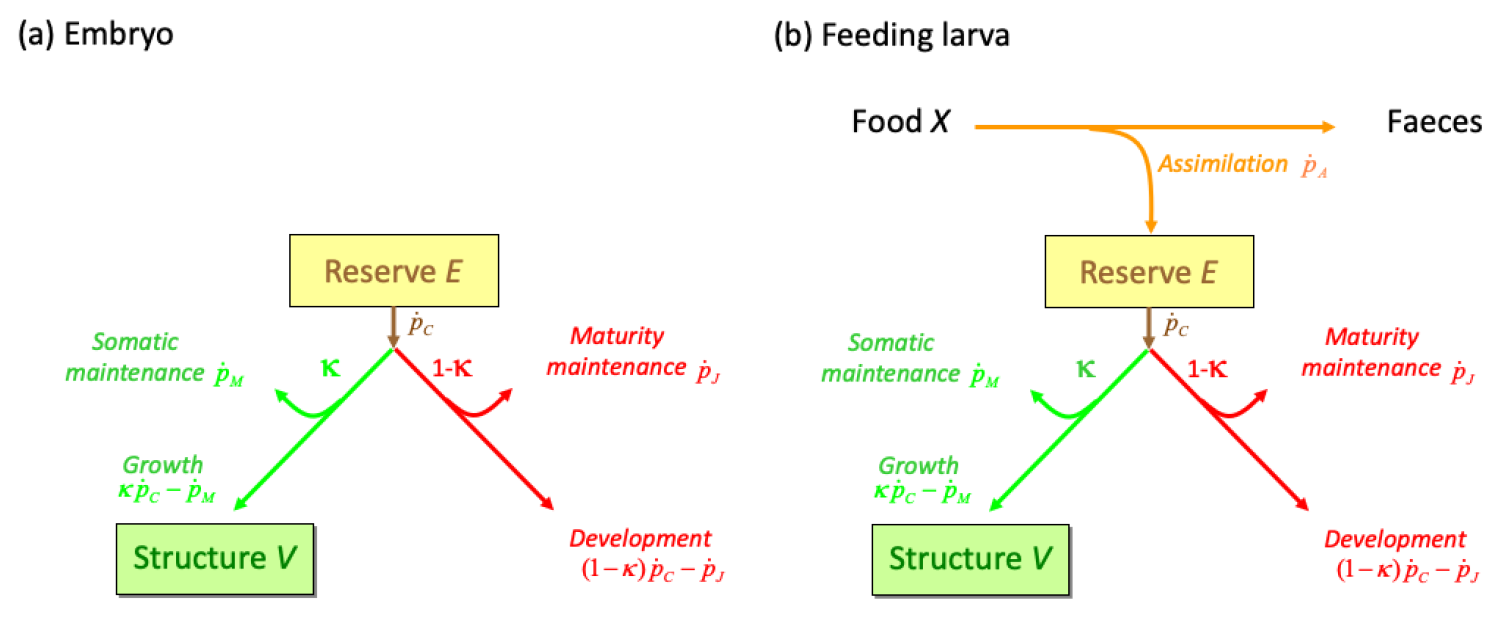
\includegraphics[width=1.0\textwidth]{figures/S1DEBflux.png}
	\centering
	\caption{Schemes of the energy fluxes of a \acrlong{deb} model (a) for the embryo stage (non-feeding stage) and (b) the feeding larval stage.}
	\label{S1DEBflux}
\end{figure}

\subsection*{Forcing variables}
\hfill \\

$T$ Temperature (K) is the water temperature surrounding an individual (modeled by CROCO-PISCES)\\

$X$ Food density averaged Mesozooplankton field ($\left[ \mu mol CL^{-1} \right]$) over the water column (modeled by CROCO-PISCES)\\

\subsection*{Initial conditions of state variables (egg stage)}

The age of the individual is set at zero on the day of spawning.\\

\begin{tabular}{|c|c|c|c|}
\hline 
Symbol  & Value      & Units  & Definition      \\ 
\hline 
$E$     & $0.99$     & $J$    & Initial Reserve \\ 
$V$     & $0.000001$ & $mm^3$ & Initial Structure\\
\hline 
\end{tabular} 

\subsection*{Primary parameters}

\begin{table}[H]
\centering
\begin{adjustbox}{width=1.2\textwidth}
\begin{tabular}{l|l|l|l}
\hline
\multicolumn{4}{l}{Primary parameters (rates are at reference temperature $T_{1} = 293 K$  ($=20$\textdegree $C$)} \\
\hline
Symbol   & Value        & Unit & Definition                                \\
\hline
$L_{h}$  & 0.28         & $cm$ & Hatch length                              \\
$L_{b}$  & 0.35         & $cm$ & Yolk-sac to feeding larva threshold       \\
$T_{A}$  & 9800         & $K$  & Arrhenius temperature                     \\
$T_{L}$  & 279/279      & $K$  & Lower temperature boundary                \\
$T_{H}$  & 294/297      & $K$  & Upper temperature boundary                \\
$T_{AL}$ & 20000/20000  & $K$  & Arrhenius temperature for lower boundary  \\
$T_{AH}$ & 95000/570000 & $K$  & Arrhenius temperature for upper boundary   \\
$K$      & 1.6          & $\mu mol CL^{-1}$ & Half-saturation constant       \\
$\kappa_{\mathrm{x}}$   & 0.71 & - & Fraction of food energy fixed in reserve \\
$\left\{\dot{p}_\mathrm{Xm} \right\}$
	& 516
	& $J.cm^{-2}.d^{-1}$
	& Maximum surface-specific ingestion rate         \\
$\left[E_{m} \right]$
	& 2700 
	& $J.cm^{-3}$
	& Maximum reserve density                         \\
$\left[E_{G} \right]$
	& 4000
	& $J.cm^{-3}$
	& Volume-specific costs of structure              \\
$\left[\dot{p}_{M} \right]$
	& 76.22 
	& $J.cm^{-3}.d^{-1}$
	& Volume-specific somatic maintenance rate\\
$\kappa$
	& 0.7
	& - 
	& Fraction of mobilized reserve allocated to growth and somatic maintenance    \\
\hline
\end{tabular}
\end{adjustbox}
\end{table}

\subsection*{Auxiliary and compounds parameters}

\begin{table}[H]
\centering
\begin{adjustbox}{width=1.2\textwidth}
\begin{tabular}{l|l|l|l}
\hline
\multicolumn{4}{l}{Auxiliary and Compounds parameters}   \\
\hline
Symbol & Value & Unit & Definition                   \\
$\delta_{M}$
	& 0.152
	& -
	& Shape coefficient                               \\
$\left \{ \dot{p}_\mathrm{Am} \right \}$
	& $\kappa_{\mathrm{x}} $ $\left \{ \dot{p}_\mathrm{Xm} \right \}=366$
	& $J.cm^{-2}.d^{-1}$
	& Maximum surface-area-specific assimilation rate\\
\hline
\end{tabular}
\end{adjustbox}
\end{table}

\subsection*{Scaled functional response}
\hfill \\

$V_{b} = (\delta_{M}L_{b})^3$ \hfill Structural volume at first-feeding in $cm^3$.\\

\textbf{if} $(V < V_{b})$ \\

$f = 0$ \hfill No feeding.\\

\textbf{else}\\

$f= \frac{X}{X+K}$	    \hfill Feeding.\\

\subsection*{Temperature correction}
\hfill \\

Each rate parameter is corrected for temperature according to the following equation \citep{Kooi2009}.\\

$
	C_{T} = exp\left ( \frac{T_{A}}{T_{1}} - \frac{T_{A}}{T} \right )
	\left ( \frac
				{1+exp\left ( \frac{T_{AL}}{T_{1}} - \frac{T_{AL}}{T_{L}} \right )
				  +exp\left ( \frac{T_{AH}}{T_{H}} - \frac{T_{AH}}{T_{1}} \right )}
				{1+exp\left ( \frac{T_{AL}}{T} - \frac{T_{AL}}{T_{L}} \right )
				  +exp\left ( \frac{T_{AH}}{T_{H}} - \frac{T_{AH}}{T} \right )}
	\right )
$\\

With $T_{1}$ the reference temperature (at which flux parameters were estimated), $T_{A}$ is the Arrhenius temperature and $T_{AH}$, $T_{AH}$, $T_{L}$, $T_{H}$ are constants used to define a curved shape of the temperature correction according to temperature.\\

$\left \{ \dot{p}_\mathrm{Am} \right \}_{T} = C_{T} \left \{ \dot{p}_\mathrm{Am} \right \}_{T_{1}}$\\

$\left [ \dot{p}_{M} \right ]_{T} = C_{T} \left [ \dot{p}_{M} \right ]_{T_{1}}$\\

\subsection*{Fluxes ($Jd^{-1}$)}
\hfill \\

$\dot{p}_\mathrm{A} = f \left \{ \dot{p}_\mathrm{Am} \right \}_{T} V^{2/3}$ \hfill Assimilation.\\

$\dot{p}_\mathrm{M} = \left [ \dot{p}_{M} \right ]_{T} V$ \hfill Volume-related somatic maintenance.\\


	$\dot{p}_{C} = \frac
					   {E\left ( \left [ E_{G} \right ] \frac{C_{T}\left \{ \dot{p}_\mathrm{Am} \right \}_{T}}{\left [ E_{m} \right ]} V^{-\frac{1}{3}}+\left [ \dot{p}_{M} \right ]_{T}\right )}
					   {\kappa\left ( \frac{E}{V} \right ) + \left [ E_{G} \right ]}$ \hfill Mobilization of energy.\\

$\dot{p}_{G} = \kappa \dot{p}_{C} - \dot{p}_\mathrm{M}$ \hfill Energy directed to structural growth.\\

$\dot{p}_{J} = V \frac{\left ( 1 - \kappa \right )}{\kappa}\left [ \dot{p}_{M} \right ]_{T}$ \hfill Maturity maintenance (for $V < V_{p}$ (Structural volume at puberty), the condition is always TRUE because in \gls{ich-deb} the complexity level of the organism at puberty is never exceeded, as we only consider embryos and larvae).\\

Starvation test\\

\textbf{if} $\kappa \dot{p}_{C} < \dot{p}_\mathrm{M}$ or $\left ( 1- \kappa \right ) \dot{p}_{C} < \dot{p}_{J}$\\

$starvation = 1$ \hfill Individual (or super-individual) removed from population.\\

\textbf{else}\\

$starvation = 0$ \hfill Individual continues in the simulation.\\

\subsection*{Differential equations}
\hfill \\

$\frac{dE}{dt} = \dot{p}_\mathrm{A} - \dot{p}_{C}$ \hfill Reserve dynamics.\\

$\frac{dV}{dt} = \frac{\dot{p}_{G}}{\left[ E_{G} \right]}$ \hfill Structure dynamics.\\

\subsection*{Integration}
\hfill \\

$E\left ( t + \Delta t \right ) = E\left ( t \right ) + \frac{dE}{dt}\Delta t$ \\

$V\left ( t + \Delta t \right ) = V\left ( t \right ) + \frac{dV}{dt}\Delta t$ \\

With $\Delta t = 0.083 d \left (=2hours\right )$

\subsection*{Observable variables}
\hfill \\

$L_{w} = \frac{V^{1/3}}{\delta_{M}}$ \hfill Physical length ($cm$).\\

where $L_{w}$ is the standard length $SL$ ($cm$), $V$ the structural volume ($cm^3$) and $\delta_{M}$ a shape coefficient.\\

We assume that the larva does not change in shape till it reaches our length criteria of $2cm(SL)$ and that there is a constant proportionality ($\delta_{M}$) between structural volume and length.\\

\clearpage
\section{Accelerated $\acrshort{deb}_{abj}$ Equations in Ichthyop-DEB model}\label{DEBabjEqn}

Jorge Flores-Valiente et al.\\

The following description is a simplification of the \gls{ringens} \acrshort{deb} model developed and with parameters estimated in this study as we only focus on the embryo and larva stages. We implemented these equations in the Lagrangian tool routines of \gls{ich} \citep{LettVerl2008} to develop \gls{ich-deb}.\\

Table \ref{param_compar} presents a comparative list of parameters used in both bioenergetic models (\textit{\gls{encrasicolus}} and \textit{\gls{ringens}}) at a reference temperature $T_{1} =  293 K$ $\left (=20\textdegree C \right )$.\\

% Tabla
\begin{table}[H]
\centering
\begin{adjustbox}{width=1.2\textwidth}
\begin{tabular}{c|c|c|c|l}
\hline
\multicolumn{5}{c}{Primary parameters (rates are at reference temperature $T_{1} = 293 K$  ($=20$\textdegree $C$)}\\
\hline
Symbol      & \textit{E. encrasicolus} & \textit{E. ringens}   & Unit   & Definition\\
\hline
$L_{1}$     & 0.28    & -        & $cm$     & Hatch length\\
$L_{2}$     & 0.35    & -        & $cm$     & Length at first-feeding\\
$E_{H}^{b}$ & -       & 0.335    & $J$      & Maturity threshold at birth\\
$E_{H}^{j}$ & -       & 83.22    & $J$      & Maturity threshold at metamorphosis\\
$E_{H}^{p}$ & -       & 42160    & $J$      & Maturity threshold at puberty\\
$L_{b}$      & - & 0.1038        & $cm$ & Volumetric length at birth (estimated at $f$ = 1)\\
$L_{j}$      & - & 0.6093        & $cm$ & Volumetric length at metamorphosis (estimated at $f$ = 1) \\
$T_{A}$     & 9800     & 10000   & $K$      & Arrhenius temperature\\
$T_{L}$     & 279      & 279     & $K$      & Lower temperature boundary\\
$T_{H}$     & 294(297) & 294(297)& $K$      & Upper temperature boundary\\
$T_{AL}$    & 20000    & 20000   & $K$      & Arrhenius temperature for lower boundary\\
$T_{AH}$    & 95000(570000)      & 95000(570000) & $K$ & Arrhenius temperature for upper boundary\\
$\kappa_{\mathrm{x}} $
	& 0.71
	& 0.8
	& -
	& Fraction of food energy fixed in reserve\\
$\left \{ \dot{p}_\mathrm{Xm} \right \}$
	& 516
	& $\left \{ \dot{p}_\mathrm{Am} \right \}/\kappa \mathrm{x} = 106(622)$
	& $J.cm^{-2}.d^{-1}$
	& \makecell[l]{Maximum surface specific ingestion rate \\ (before and after metamorphosis for \textit{E. ringens})} \\
$\left \{ \dot{p}_\mathrm{Am} \right \}$
	& $ \kappa \mathrm{x} \left \{ \dot{p}_\mathrm{Xm} \right \}= 366$
	& 84.97(498)
	& $J.cm^{-2}.d^{-1}$
	& \makecell[l]{Surface-area-specific maximum assimilation rate \\ (before and after metamorphosis for \textit{E. ringens})} \\
$\left[ E_{m} \right]$ 
	& 2700
	& $\left \{ \dot{p}_\mathrm{Am} \right \}/\dot{v}=2060$
	& $J.cm^{-3}$ & Maximum reserve density\\
$\left[ E_{G} \right]$
	& 4000
	& 5283
	& $J.cm^{-3}$ & Volume-specific costs of structure\\
$\left [ \dot{p}_{M} \right ]$
	& 76.22
	& 79.95
	& $J.cm^{-3}.d^{-1}$
	& Specific Volume-linked somatic maintenance rate\\
$\kappa$
	& 0.7 
	& 0.5512 
	& - 
	& Fraction of mobilized reserve allocated to soma\\
$\dot{k}_{J}$ & - & 0.002 	        & $d^{-1}$     & Maturity maintenance rate coefficient\\
$\dot{v}$
	& - & 0.04124(0.2421)
	& $cm. d^{-1}$ 
	& \makecell[l]{Energy conductance \\ (before and after metamorphosis for \textit{E. ringens})}\\
$\delta_{M}$
	& 0.152
	& 0.1889
	& -
	& Shape coefficient for larvae\\
\end{tabular}
\end{adjustbox}
\end{table}


\subsection*{Forcing variables}
\hfill \\

$T$ Temperature (K) is the water temperature surrounding an individual (modeled by CROCO-PISCES)\\

$X$ Food density averaged Mesozooplankton field ($\left[ \mu mol CL^{-1} \right]$) over the water column (modeled by CROCO-PISCES)\\

\subsection*{State variables – Initial conditions}

The age of the individual is set at zero on the day of spawning.\\

\begin{tabular}{|c|c|c|c|}
\hline 
Symbol  & Value      & Units  & Definition      \\ 
\hline 
$E$     & $0.99$     & $J$    & Initial Reserve \\ 
$V$     & $0.000001$ & $mm^3$ & Initial Structure\\
$E_{H}$ & $0$ 		  & $J$    & Cumulated energy invested into development\\
$E_{R}$ & $0$         & $J$   & Reproduction buffer\\
\hline 
\end{tabular}

\subsection*{Scaled functional response}
\hfill \\

\textbf{if} $(E_{H} < E_{H}^b)$\\

$f = 0$				\hfill No feeding.\\

\textbf{else}\\

$f= \frac{X}{X+K}$	\hfill Feeding.\\

\subsection*{Temperature correction}
\hfill \\

Each rate parameter is corrected for temperature according to the following equation \citep{Kooi2009}.\\

$
	C_{T} = exp\left ( \frac{T_{A}}{T_{1}} - \frac{T_{A}}{T} \right )
	\left ( \frac
				{1+exp\left ( \frac{T_{AL}}{T_{1}} - \frac{T_{AL}}{T_{L}} \right )
				  +exp\left ( \frac{T_{AH}}{T_{H}} - \frac{T_{AH}}{T_{1}} \right )}
				{1+exp\left ( \frac{T_{AL}}{T} - \frac{T_{AL}}{T_{L}} \right )
				  +exp\left ( \frac{T_{AH}}{T_{H}} - \frac{T_{AH}}{T} \right )}
	\right )
$\\

With $T_{1}$ the reference temperature (at which flux parameters were estimated), $T_{A}$ is the Arrhenius temperature and $T_{AH}$, $T_{AH}$, $T_{L}$, $T_{H}$ are constants used to define a curved shape of the temperature correction according to temperature.\\

$\left \{ \dot{p}_\mathrm{Am} \right \}_{T} = C_{T} \left \{ \dot{p}_\mathrm{Am} \right \}_{T_{1}}$\\

$\left [ \dot{p}_{M} \right ]_{T} = C_{T} \left [ \dot{p}_{M} \right ]_{T_{1}}$\\


Temperature correction now affects two additional parameters.\\

$\dot{v}_{T} = C_{T} \dot{v}_{T_{1}}$\\

$\dot{K}_{jT} = C_{T} \dot{K}_{jT_{1}}$\\

\subsection*{Metabolic acceleration}
\hfill \\

Only two parameters are impacted by growth acceleration.\\

\textbf{if}	$E_{H} < E_{H}^b$\\

$S_{M} = 1$ \hfill No acceleration.\\

\textbf{else if} $E_{H}^b < E_{H} < E_{H}^j$\\

$S_{M} = \frac{L}{L_{b}}$ \hfill Acceleration.\\

\textbf{else}\\

$S_{M} = \frac{L_{j}}{L_{b}}$ \hfill Constant growth.\\

The $S_{M}$ parameter only accelerates growth from birth to metamorphosis.\\

$\left \{ \dot{p}_\mathrm{Am} \right \}_{S_{M}} = S_{M} \left \{ \dot{p}_\mathrm{Am} \right \}_{T}$\\

$\dot{v}_{S_{M}} = S_{M} \dot{K}_{jT}$\\

\subsection*{Fluxes ($Jd^{-1}$)}
\hfill \\

\textbf{if}	$E_{H} < E_{H}^b$\\

$\dot{p}_\mathrm{A} = 0$ \hfill No assimilation.\\

\textbf{else}\\

$\dot{p}_\mathrm{A} = f \left \{ \dot{p}_\mathrm{Am} \right \}_{S_{M}} V^{2/3}$ \hfill Assimilation.\\

\hfill \\

$\dot{p}_\mathrm{M} = \left [ \dot{p}_{M} \right ]_{T} V$ \hfill Volume-related somatic maintenance.\\

$\dot{p}_{C} = \frac{E}{V}*\frac{\left [ E_{G} \right ]\dot{v}_{S_{M}}V^{2/3}+\left [ \dot{p}_{M} \right ]_{T}}{\kappa\frac{E}{V}+\left [ E_{G} \right ]}$ \hfill Mobilization of energy.\\

$\dot{p}_{J} = \dot{K}_{jT} E_{H}$ \hfill Maturity maintenance.\\

\subsection*{Differential equations}
\hfill \\

$\frac{dE}{dt} = \dot{p}_\mathrm{A} - \dot{p}_{C}$ \hfill Reserve dynamics.\\

$\frac{dV}{dt} = \frac{\kappa \dot{p}_{C} - \dot{p}_\mathrm{M}}{\left[E_{G} \right]}$\\

\textbf{if} $E_{H} < E_{H}^p$\\

$\frac{dE_{H}}{dt} = (1 - \kappa) \dot{p}_{C} - \dot{p}_{J}$\\

$\frac{dE_{R}}{dt} = 0$\\

\textbf{else}\\

$\frac{dE_{H}}{dt} = 0$\\

$\frac{dE_{R}}{dt} = (1 - \kappa) \dot{p}_{C} - \dot{p}_{J}$\\

\subsection*{Integration}
\hfill \\

$E\left ( t + \Delta t \right ) = E\left ( t \right ) + \frac{dE}{dt}\Delta t$ \\

$V\left ( t + \Delta t \right ) = V\left ( t \right ) + \frac{dV}{dt}\Delta t$ \\

$E_{H}\left ( t + \Delta t \right ) = E_{H}\left ( t \right ) + \frac{dE_{H}}{dt}\Delta t$ \\

$E_{R}\left ( t + \Delta t \right ) = E_{R}\left ( t \right ) + \frac{dE_{R}}{dt}\Delta t$ \\

With $\Delta t = 0.083 d \left (=2hours\right )$

\subsection*{Observable variables}
\hfill \\

$L_{w} = \frac{V^{1/3}}{\delta_{M}}$ \hfill Physical length ($cm$).\\

where $L_{w}$ is the standard length $SL$ ($cm$), $V$ the structural volume ($cm^3$) and $\delta_{M}$ a shape coefficient.\\

We assume that the larva does not change in shape till it reaches our length criteria of $2cm(SL)$ and that there is a constant proportionality ($\delta_{M}$) between structural volume and length.\\


\end{document}
%%%%%%%%%% END DOCUMENT %%%%%%%%%%